\RequirePackage{fix-cm}
%
\documentclass{svjour3}                     % onecolumn (standard format)
% To have symmetric margin (only for research note)
\setlength{\textwidth}{\dimexpr\pdfpagewidth-2in}% Equal left/right margins
%\documentclass[smallcondensed]{svjour3}     % onecolumn (ditto)
%\documentclass[smallextended]{svjour3}       % onecolumn (second format)
%\documentclass[twocolumn]{svjour3}          % twocolumn
%
\smartqed  % flush right qed marks, e.g. at end of proof
%

\usepackage{uclrn}
\usepackage{newtxtext}
\usepackage{newtxmath}
\usepackage[round]{natbib} 
%\setcitestyle{aysep={}} 

\newcommand\fscore{\operatorname{F-score}}
\usepackage{graphicx}
\usepackage{tabularx}
\usepackage{listings}
\usepackage{float}
\usepackage{multirow}
\usepackage{mathtools}
\usepackage{makecell}
\usepackage{algorithm}
%\usepackage{cleveref}
\usepackage{algpseudocode}
\usepackage{pifont}
%\usepackage{cite}
\usepackage{verbatim}
\usepackage{enumitem}
\usepackage{url}
%\usepackage{microtype}
\usepackage{caption}
\usepackage{booktabs} % For formal tables
\usepackage{subcaption}
\usepackage[misc,geometry]{ifsym} 
\usepackage{etoolbox}
\usepackage[colorlinks=true,allcolors=blue]{hyperref}

\captionsetup{compatibility=false}

\rnnumber{17/xx}
%\usepackage[table]{xcolor}% http://ctan.org/pkg/xcolor
%\newtheorem{definition}{Definition}

\lstset{language=Java,tabsize=2,basicstyle=\ttfamily\scriptsize} 

\newcommand\FIXME[1]{\textbf{FIXME: #1}}

\begin{document}

\title{Awareness of Stack Overflow Users to\\ Outdated and License-violating Code:\\ The Online Survey}
%\subtitle{Do you have a subtitle?\\ If so, write it here}

\titlerunning{SO Developers awareness: Outdated and License-violating Code}        % if too long for running head

\author{Chaiyong~Ragkhitwetsagul, Jens~Krinke}

%\authorrunning{Short form of author list} % if too long for running head

\institute{Chaiyong Ragkhitwetsagul~(\Letter), Jens Krinke \at
              Computer Science Department., University College London, UK \\
              Tel.: +44 (0)20 7679,  Fax: +44 (0)20 7387 1397\\
              \email{\{ucabagk, j.krinke\}@ucl.ac.uk}           %  \\
%             \emph{Present address:} of F. Author  %  if needed}
}

\date{\today}
% The correct dates will be entered by the editor


\maketitle

\begin{abstract}
ABSTRACT GOES HERE
\end{abstract}

\section{Introduction}

Outdated third-party code and software licensing conflicts are ramifications by
reusing source code by copying and pasting (i.e.~code cloning). \cite{Xia2014}
show that a large number of open source systems reuse outdated third-party
libraries from popular open source projects. Using the outdated code give
detrimental effects to the software since they may introduce vulnerabilities. On
the other hand, \cite{German2009} found conflicts in software license between
the clones among different systems that come from the same source,~i.e.~clone
siblings.

The Internet encourages fast and easy way of sharing and copying code.
Developers nowadays do not only copy code from local software projects, but also
from online sources such as programming Q\&A website and online code
repositories. Stack Overflow is one of the most popular programming Q\&A
websites in the word. It has 7.6 million users, 14 million questions, 23 million
answers\footnote{Data as of 21 August 2017
	from~\url{https://stackexchange.com/sites}}, and more than 50 million developers
visiting each month\footnote{Data as of 21 August 2017 from:
	\url{https://stackoverflow.com}}. Nevertheless, several code snippets on Stack
Overflow are found to be problematic. Many code snippets provided as solutions
are workarounds and occasionally contains defects or vulnerabilities.
\cite{Acar2016} performed a user study and found that Stack Overflow helps
developers to solve Android programming problems quicker than other resources
while, at the same time, offers less secure code than books or the official
Android documentation. Only 17\% of the Stack Overflow discussion threads the
participant visited during the study contain secure code snippets. They also
found that similar piece of API call copied from Stack Overflow by participants
in their study existed in a random sample of 200,000 Android apps from Google
Play. \cite{An2017} showed that 1,279 cloned snippets between 399 Android apps
and Stack Overflow potentially violate software licenses.

We are interested in studying the issues of outdated code and software license
violation cause by code snippets on Stack Overflow. Asking and answering
questions on Stack Overflow usually involve copying and pasting source code
snippets, either in a question or an answer. However, the copied snippets are
not regularly checked and occasionally not up-to-date with their originals. Some
snippets are copied from an open source system with stricter software license
than Stack Overflow's Attribution-ShareAlike 3.0 Unported (CC BY-SA 3.0). Before
this study, we performed an preliminary study using code clone detection tools
to locate cloned code snippets in accepted answers. We found that many snippets
were copied from open source projects. Some cloned snippets are outdated and
possibly violating the original software license. In either case, these snippets
are potentially harmful for reuse. To accompany the findings and to gain
insights into the cause of this problem, we resort to a qualitative study using
an online survey of Stack Overflow developers who 1) answer programming
questions with code snippets and 2) reuse code snippets from Stack Overflow
answers. 

In this paper, we use the term ``answerers'' to refer to Stack Overflow users
who have high reputation, specifically the users with reputation from 963,731
(highest)  to 6,999. The answerers gain their reputation from answering
questions and receiving votes from other users. The reputation reflects trust
they gain from other users and their activeness in answering questions. We ask
the answerers the origins of source code snippets in their answers  and assess
their awareness of outdated and licensed code. 
%We use the term ``visitors'' the
%refer to developers, who may or may not have a Stack Overflow account but visit
%Stack Overflow when facing programming problems. They copy example code snippets
%that are relevant to their problems and reused them in their software. 
%We ask Stack Overflow visitors, who copied code snippets from
%Stack Overflow, about their experience of outdated or license-violating code.

\section{Research Questions}
In this study, we would like to answer the following
research questions:

\begin{enumerate}
	\item \textbf{RQ1 (Sources of Stack Overflow Answer Snippets):} \textit{Where are the code snippets in Stack Overflow answers from?}
	\item \textbf{RQ2 (Awareness of Stack Overflow answerers to outdated code):} \textit{Are Stack Overflow answerers aware of outdated code in their answers?}
	\item \textbf{RQ3 (Awareness of Stack Overflow answerers to outdated code):} \textit{Are Stack Overflow answerers aware of outdated code in their answers?}
%	\item \textbf{RQ4(Awareness of Stack Overflow visitors to outdated code):} \textit{Are Stack Overflow visitors aware of outdated code on Stack Overflow?}
%	\item \textbf{RQ5 (Awareness of Stack Overflow visitors to software licensing conflicts):} \textit{Are Stack Overflow visitors aware of of software licensing conflicts caused by reusing code snippets from Stack Overflow?}
\end{enumerate}

\section{Research Methodology}
The study is performed using an online survey. We designed the survey using
Google Forms by following the principles of survey research
by~\cite{Pfleeger2001} and~\cite{Kitchenham2002}. 
%We created two versions of the
%survey: \textbf{the answerer survey}, and, \textbf{the visitor survey}. 
The survey is completely anonymous and the participants could decide to leave at
any time. It does not collect any sensitive personal information from the
participants and were approved for an ethical waiver by the designated ethics
officer in the Computer Science Department at UCL.  The complete version of
the survey can be found in the Appendix~\ref{appendixA}.


\subsection{The Survey Design}
The Stack Overflow answerer survey contains 11 questions: 7 Likert's scale
questions, 3 yes/no questions, and one open-ended question for additional
comments. The first two questions were mandatory while the other 9 questions
were shown to the participants based on their previous answers. The survey collects
information of the participant's software development experience, experience of
answering Stack Overflow questions, sources of the Stack Overflow snippets,
concerns of copying code snippets to Stack Overflow, problems from code 
snippets on Stack Overflow, fixing outdated code, and additional feedbacks.

\subsection{Participants}

\begin{table}
	\centering
	\caption{The Stack Overflow answerer taken the surveys}
	\label{tab:answerers}
	\begin{tabular}{lrrrr}
		\toprule
		Target group & Reputation & Sent emails & Answers & Rate \\
		\midrule
		Answerer Group 1 & 963,731--7,674 & 300 & 113 & 38\% \\
		Answerer Group 2 & 7,636--6,999 & 307 & 85 & 28\% \\
		\midrule
		Total & -- & 607 & 198 & 33\% \\
		\bottomrule
	\end{tabular}
\end{table}

We selected the participants for our answerer survey based on their Stack Overflow reputation. On
Stack Overflow, a user's reputation reflects how much the community trust the
user. A user earns reputation when he or she receives up votes for good
questions and useful answers. Accepted answers receive more reputation score
than questions, and regular answers\footnote{Stack Overflow
	Reputation:~\url{https://stackoverflow.com/help/whats-reputation}}. Thus, Stack
Overflow reputation is an indicator of user's skills and their involvement in
asking and answering questions on the site.

The participants were invited to take the survey via email addresses publicly available on their
public Stack Overflow and GitHub profiles. We selected the answerers based on
all-time reputation ranking\footnote{Stack Overflow Users (data as of 25 July
	2017):~\url{https://stackoverflow.com/users?tab=Reputation&filter=all}} and
separated them into two groups (see Table~\ref{tab:answerers}) so that we can
compare the results or observe similar patterns between them. 
The first group had reputation from 963,731 (the
highest) to 7,674, and the second group had reputation from 7,636 to 6,999 which
we sent out 300 and 307 emails (excluding undelivered ones) respectively. The
survey was open for participation for a month, from 25 July 2017 to 25 August
2017, before we collected and analysed the responses.

%\subsection{The Visitor Survey}
%
%The Stack Overflow visitor survey is consisted of 16 questions: 9 Likert's scale
%questions, 3 yes/no questions, 2 multiple-choice questions, and 2 open-ended
%questions. The first four questions were mandatory while the other 12 questions
%were shown to the participants based on their previous answers. The survey collects
%information of the participant's software development experience, importance of
%Stack Overflow, reasons for reusing Stack Overflow snippets, problems from
%Stack Overflow snippets, licensing of code on Stack Overflow, and additional
%feedbacks.
%
%\begin{table}
%	\centering
%	\caption{The Stack Overflow visitors taken the survey}
%	\label{tab:visitors}
%	\begin{tabular}{lr}
%		\toprule
%		Invitation channels & Answers \\
%		\midrule
%		Chaiyong's Facebook post & 47 \\
%		Blognone.com & 32 \\
%		University of Molise & 6 \\
%		comp.lang.java.programmer & 3 \\
%		Software Engineering Facebook page & 1 \\
%		\midrule
%		Total & 89 \\
%		\bottomrule
%	\end{tabular}
%\end{table}
%
%The participants for this survey were invited to take the survey via five
%channels. The first channel is via the first author's Facebook post where the
%first author invited friends who are software developers and have experience of
%copying code snippets from Stack Overflow to take the survey. The second channel
%is a popular Thai technology news and media community called blognone.com which
%attracts a high number of software developers. The first author posted an
%invitation to the visitor survey in a discussion forum. The third channel
%collects answers from University of Molise which is the third author's
%workplace. The last two channels are from a comp.lang.java.programmer Google
%groups and Software Engineering Facebook page. The survey was open for
%participation for a month, from 25 July 2017 to 25 August 2017, before we
%collected and analysed the responses. The number of participants taken the
%survey are shown in Table~\ref{tab:visitors}.

\section{Results and Discussions}

%\subsection{Answerer Responses}
We received 113 answers (38\% response rate) from the first group and 85 answers
(28\% response rate) from the second group of Stack Overflow answerers. The response
rate from both groups were high considered other online survey in software
engineering that received approximately 14--20\%~\FIXME{double-check the
	citation again for the magic numbers.}~\citep{Punter2003}.

\subsubsection*{General Information}
%General information of the answerers' experience and frequency of answering 
%questions on Stack Overflow with code snippets as discussed below.

%\subsubsection*{Q1: How long have you been working on developing software?}

\begin{figure}
	\begin{subfigure}{.5\textwidth}
		\centering
		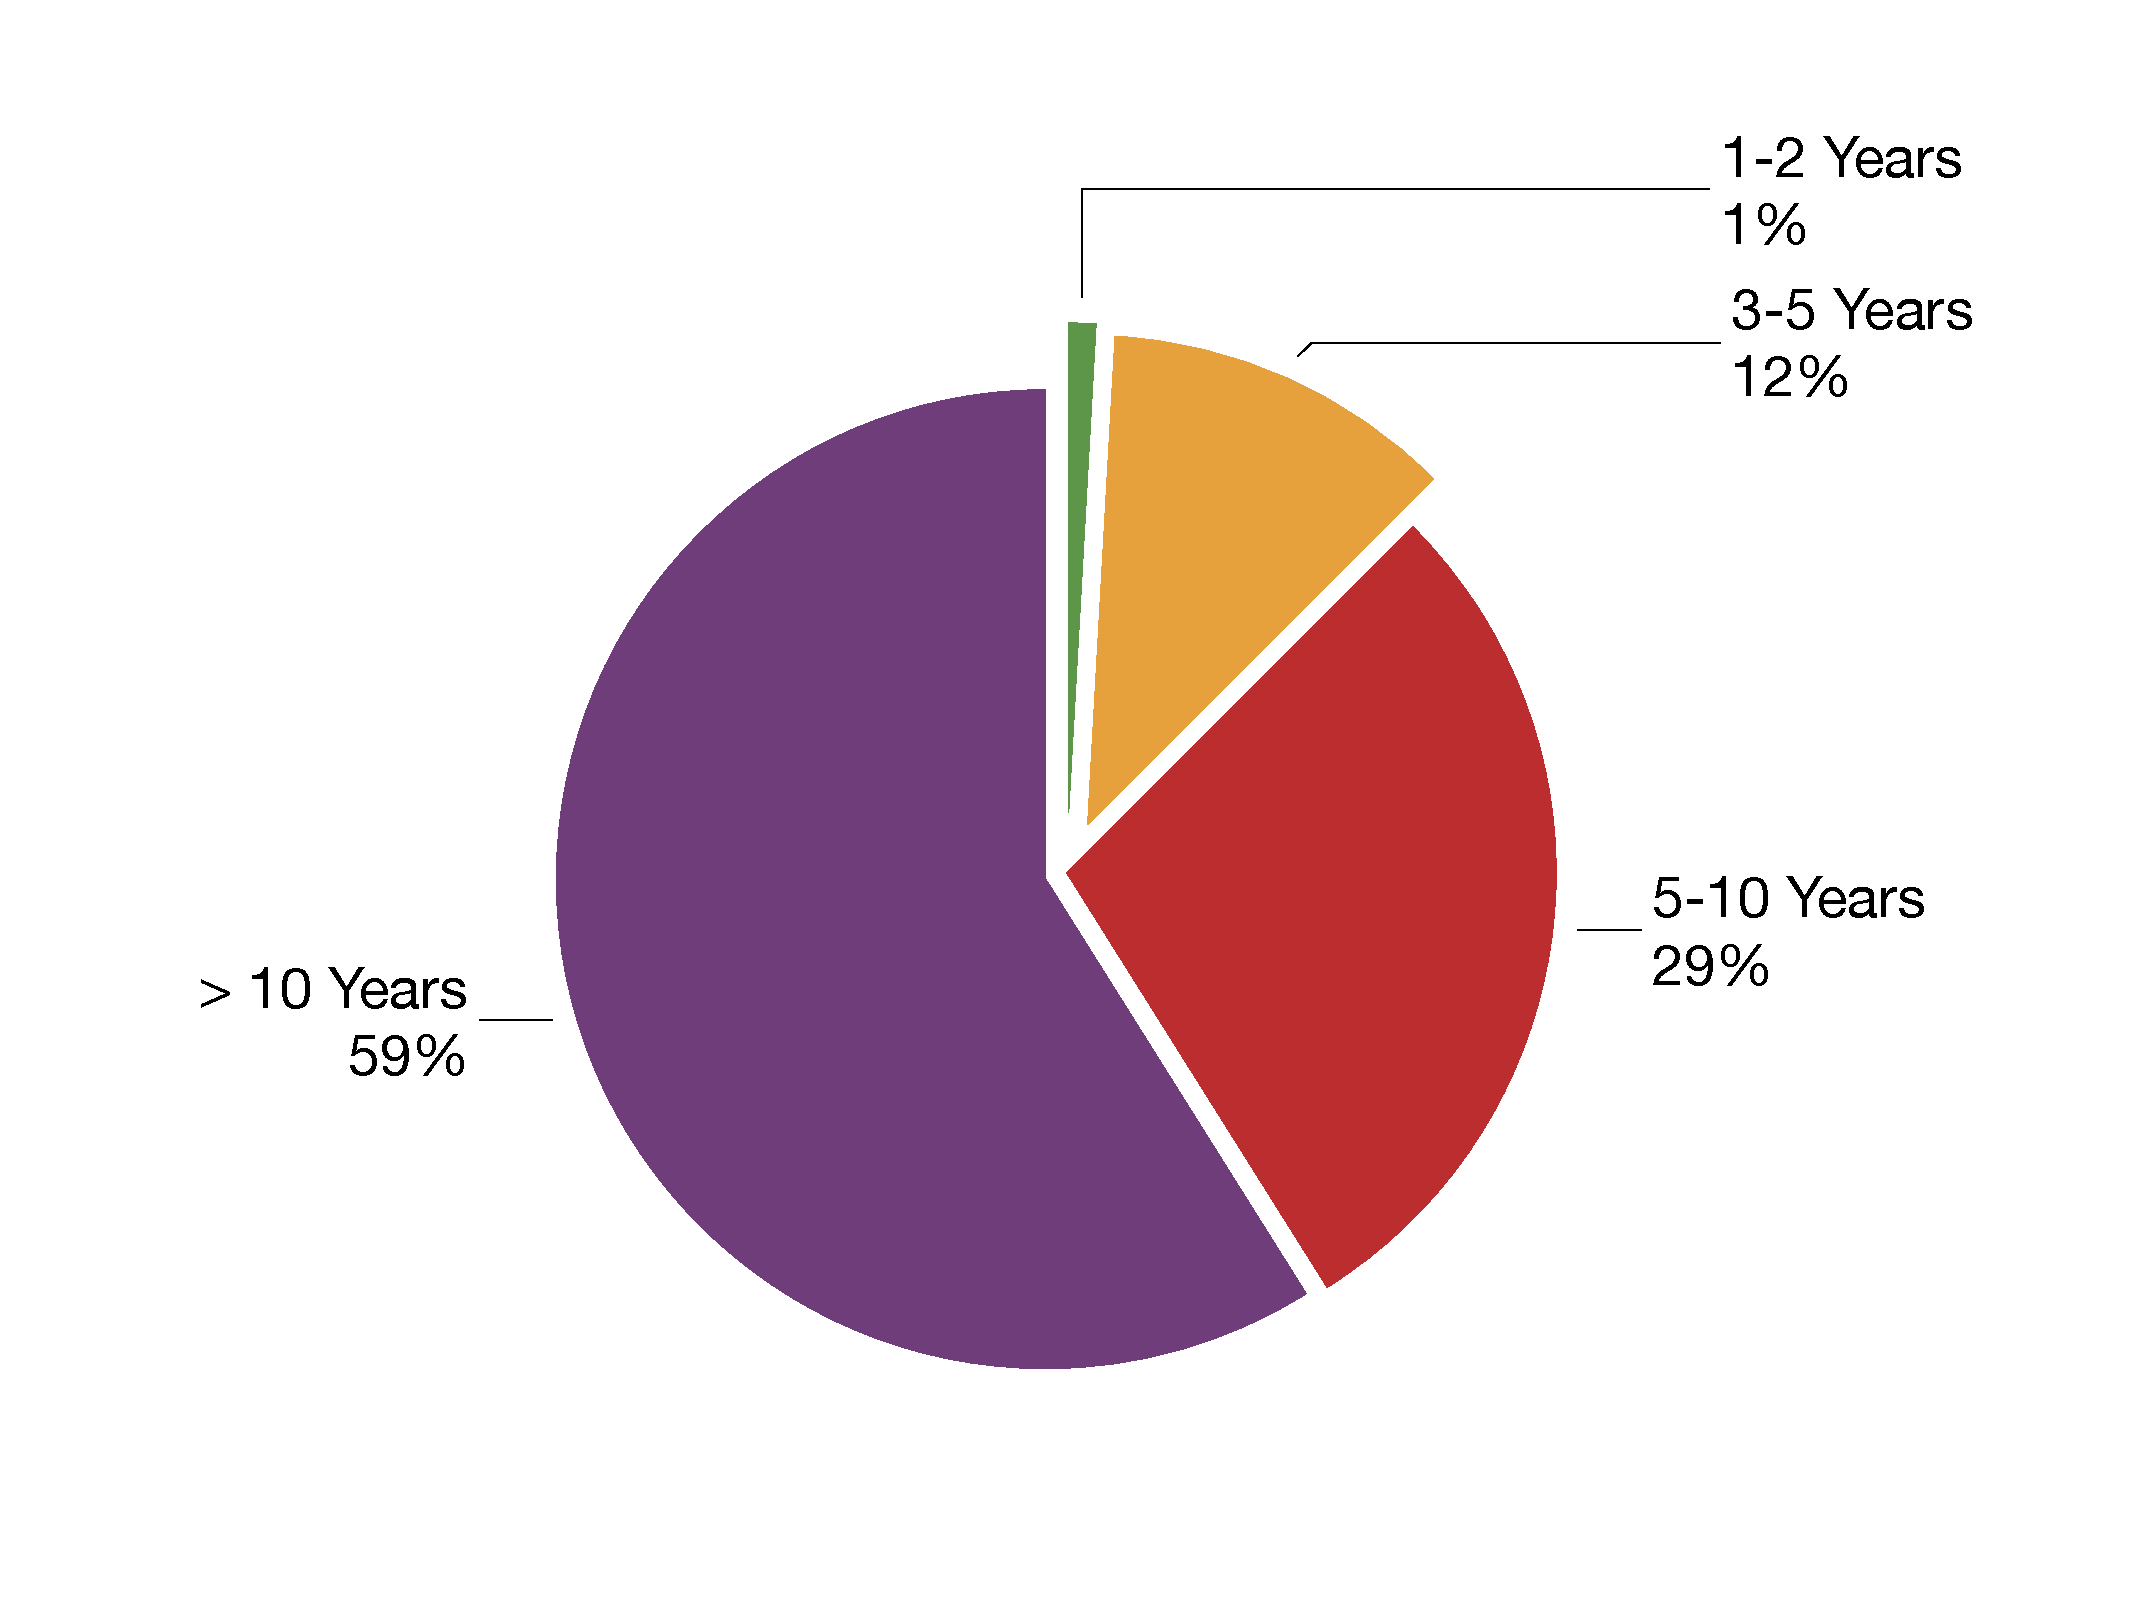
\includegraphics[width=0.8\linewidth]{survey_exp_1}
		\caption{Group 1}
		\label{fig:survey_group1_exp}
	\end{subfigure}%
	\begin{subfigure}{.5\textwidth}
		\centering
		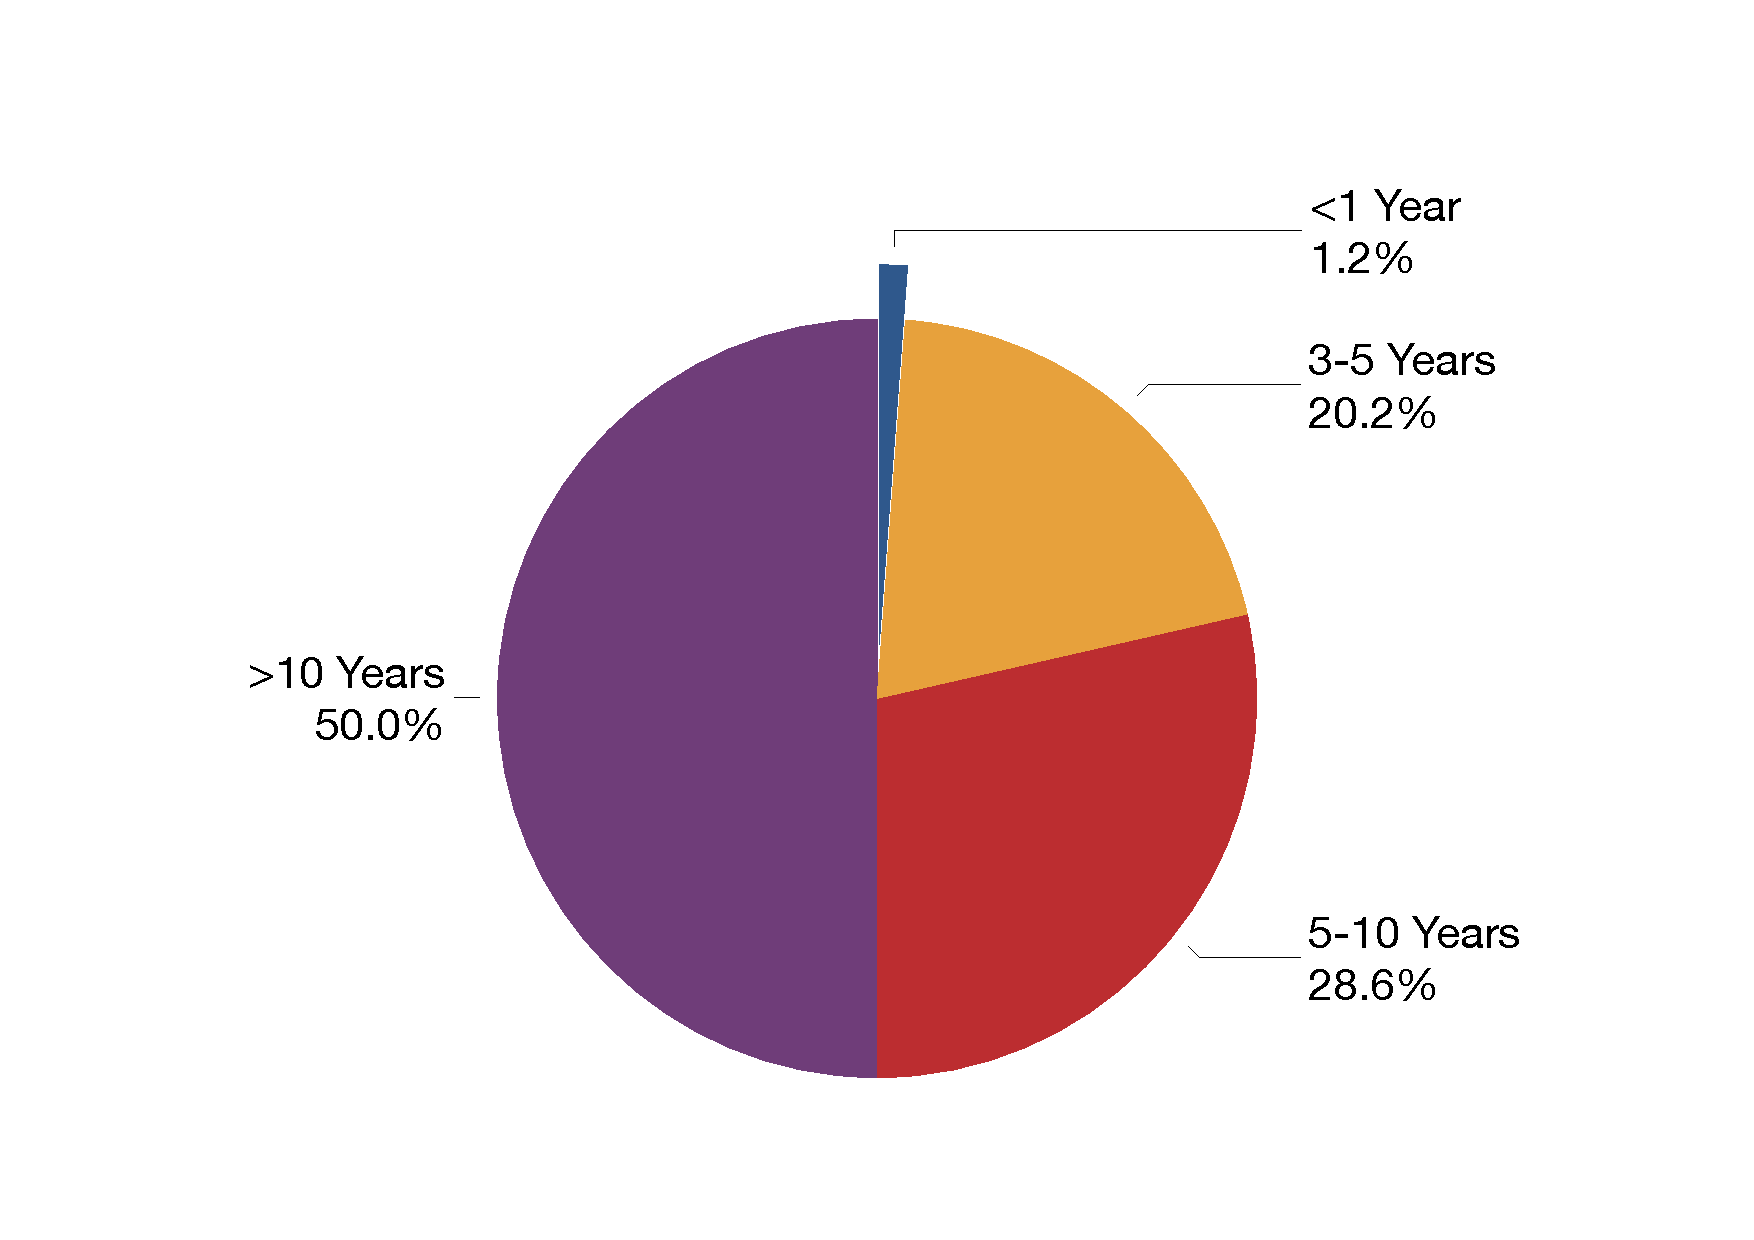
\includegraphics[width=0.8\linewidth]{survey_exp_2}
		\caption{Group 2}
		\label{fig:survey_group2_exp}
	\end{subfigure}
	\caption{Experience of the Stack Overflow answerers}
	\label{fig:survey_exp}
\end{figure}

The majority of users in both groups are experienced developers 
with more than 10 years of experience or between 5 to 10 years 
as depicted in Figure~\ref{fig:survey_exp}. There are 59\% of the answerers in Group 1 that have more than 10 year of software development experience, while a slightly less percentage of 50\% in Group 2.

The participants are active users and regularly answer questions on Stack Overflow (see Figure~\ref{fig:survey_answer_frequency}). Ninety two (81\%) and fifty one (61\%) of answerers from Group 1 and Group 2  answer questions at least once a week.

More than half of the answerers very frequently (81--100\% of the time) or frequently (61--80\% of the time) include code snippets in their answers. To break down into two groups as depicted in Figure~\ref{fig:survey_answer_frequency_with_code},
Group 1 very frequently (48.7\%) and frequently (27.4\%) provide code examples when answering. Likewise, Group 2 does the same (very frequently for 32.1\% and frequently for 36.9\%).

%\subsubsection*{How frequently do or did you answer questions on Stack Overflow?}

\begin{figure}
		\centering
		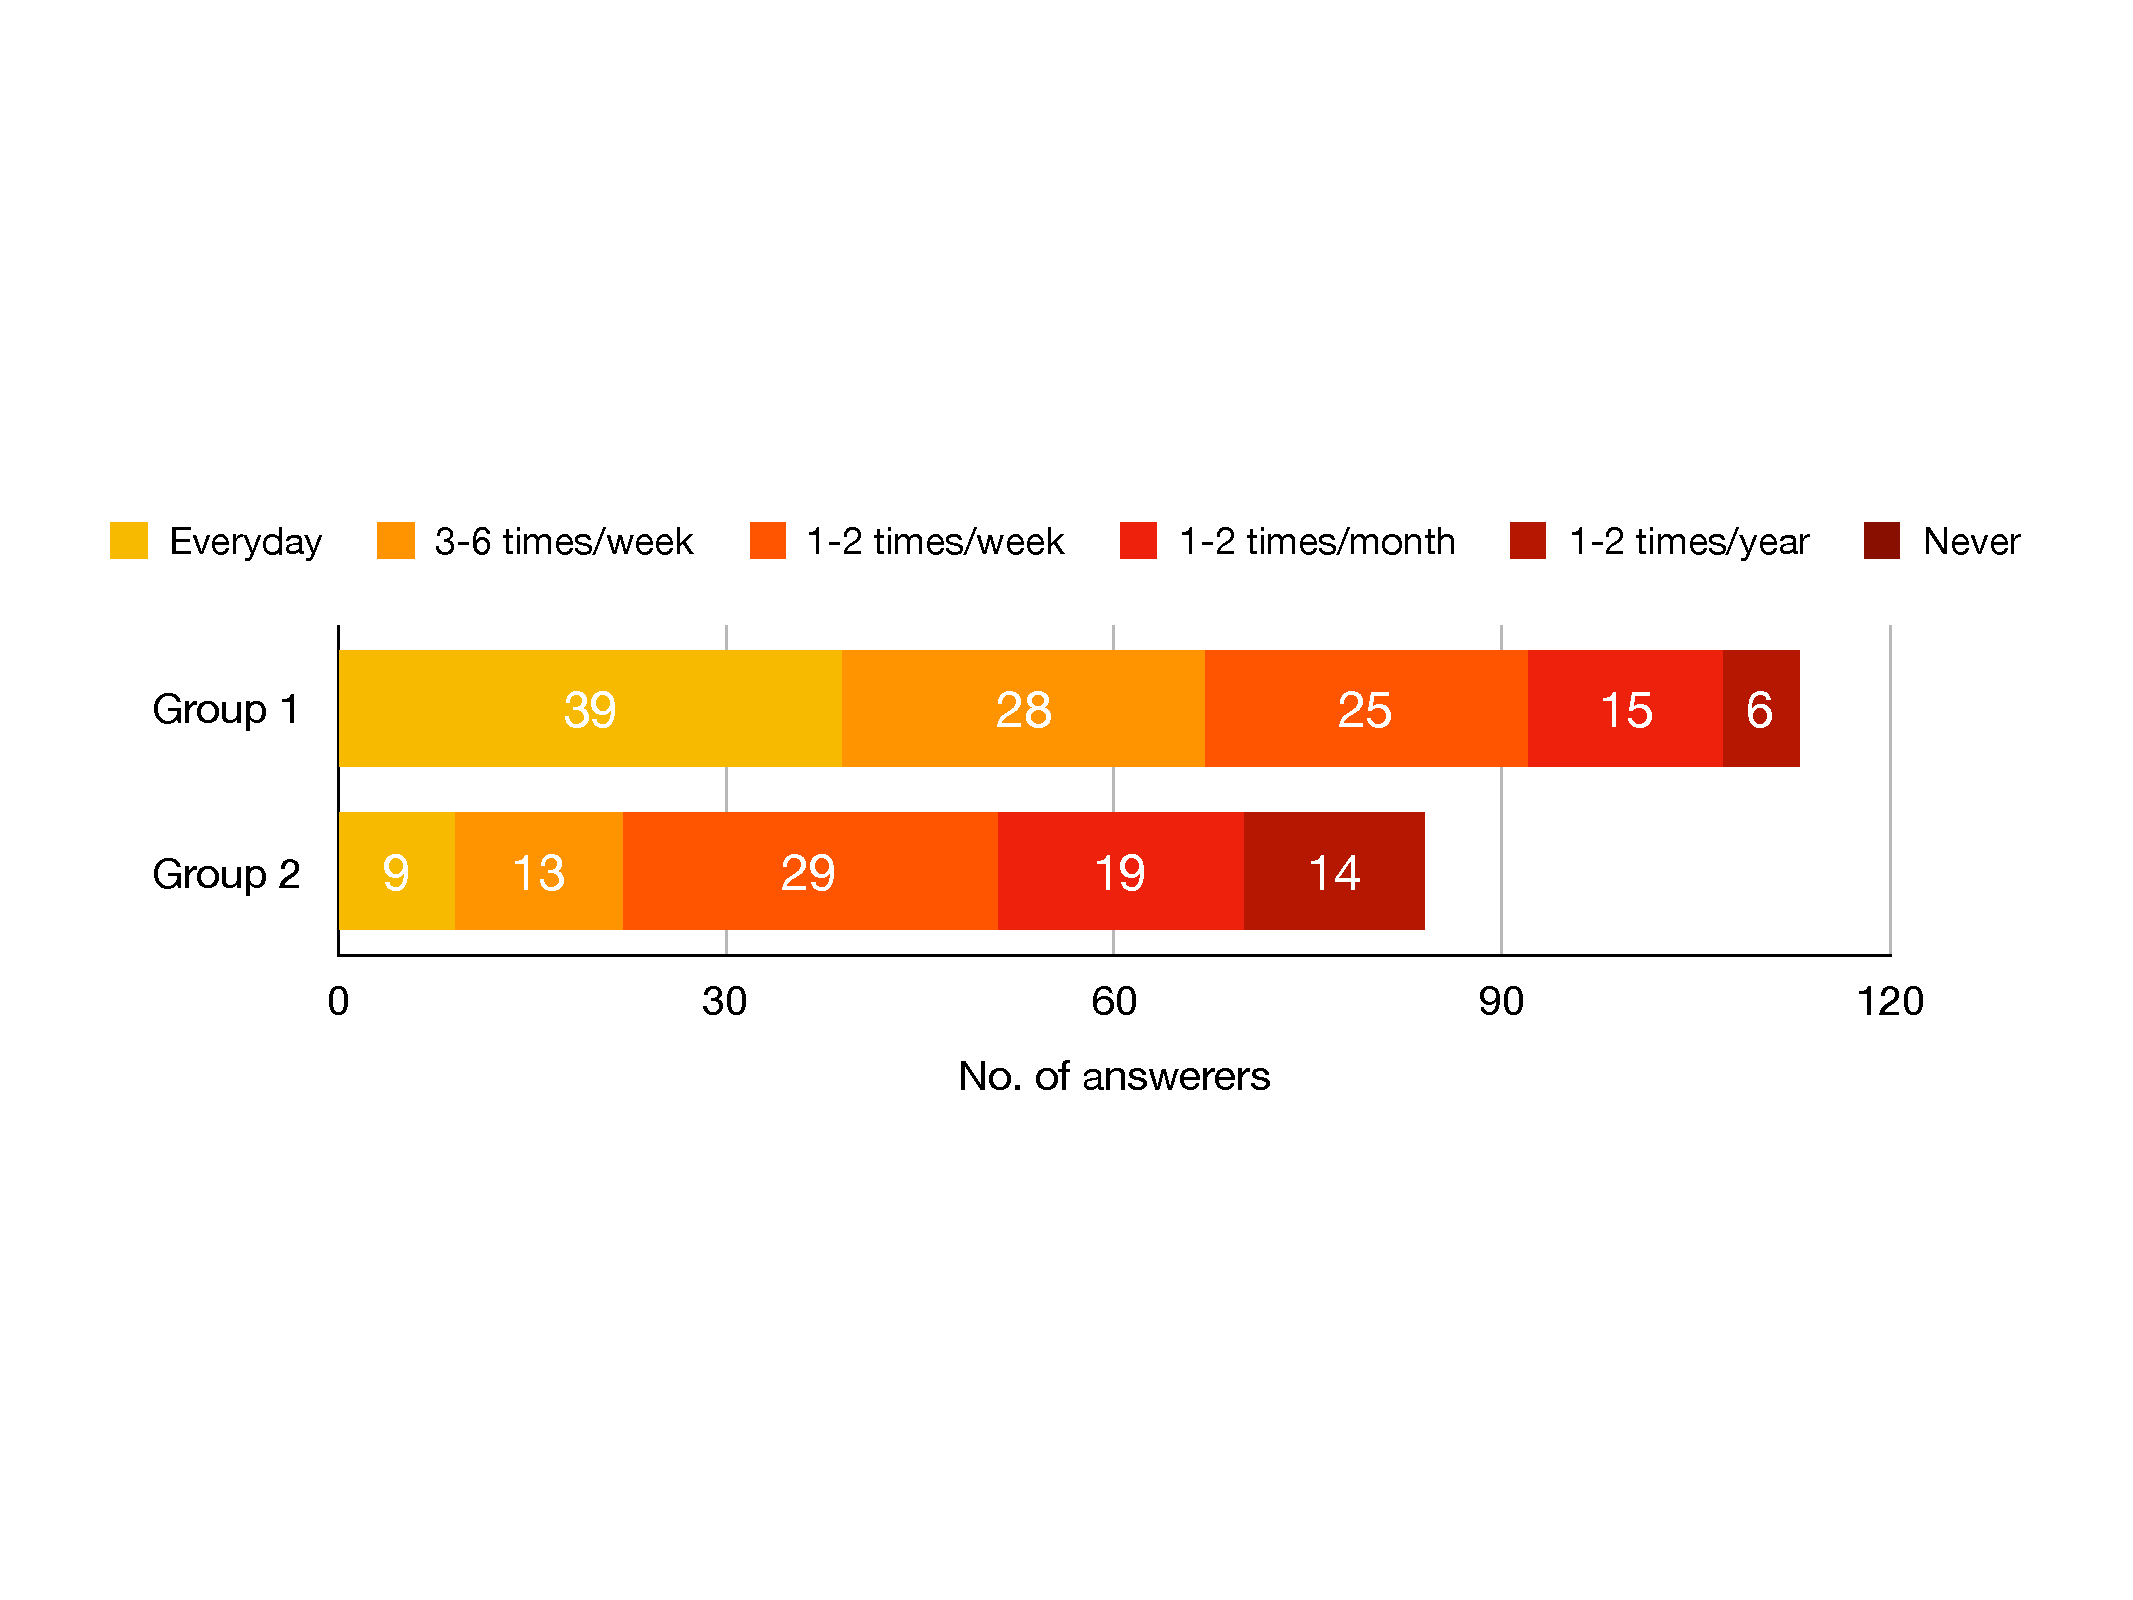
\includegraphics[width=0.8\linewidth]{survey_answer_frequency}
		\caption{Frequency of answering questions}
		\label{fig:survey_answer_frequency}
\end{figure}

%\subsubsection*{How frequently do or did you include code snippets in your answers on Stack Overflow?}

\begin{figure}
	\begin{subfigure}{.5\textwidth}
		\centering
		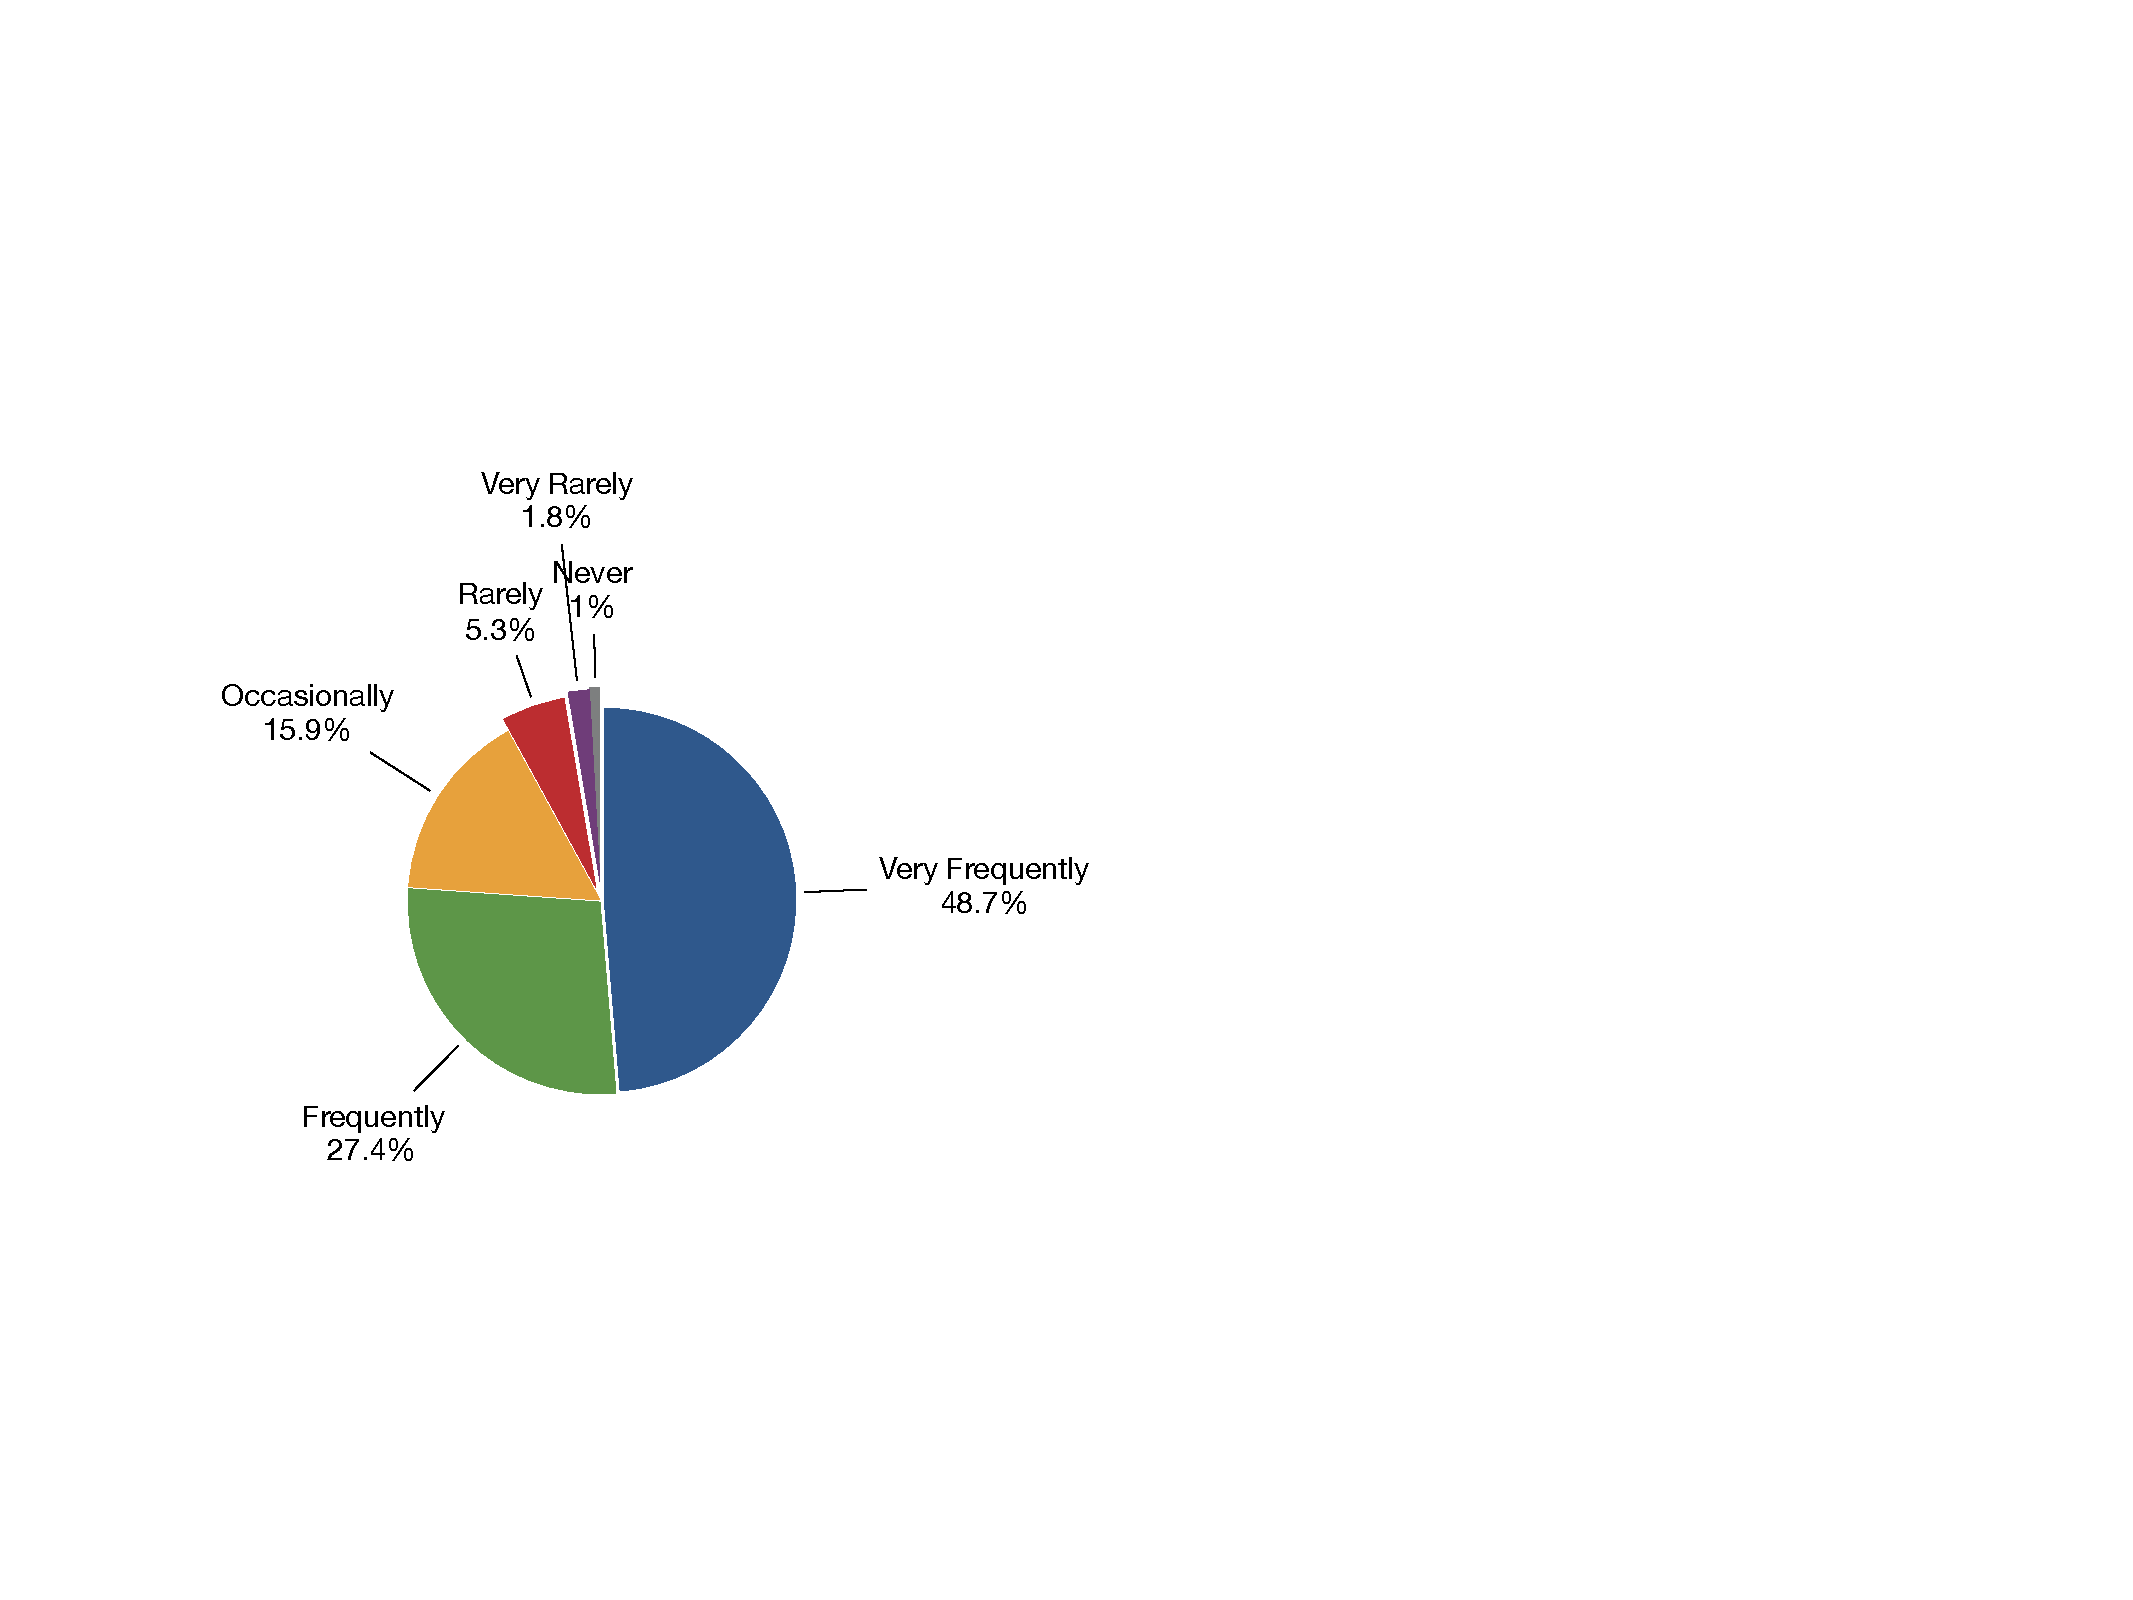
\includegraphics[width=\linewidth]{survey_answer_frequency_with_code_1}
		\caption{Group 1}
		\label{fig:survey_answer_frequency_with_code_1}
	\end{subfigure}%
	\begin{subfigure}{.5\textwidth}
		\centering
		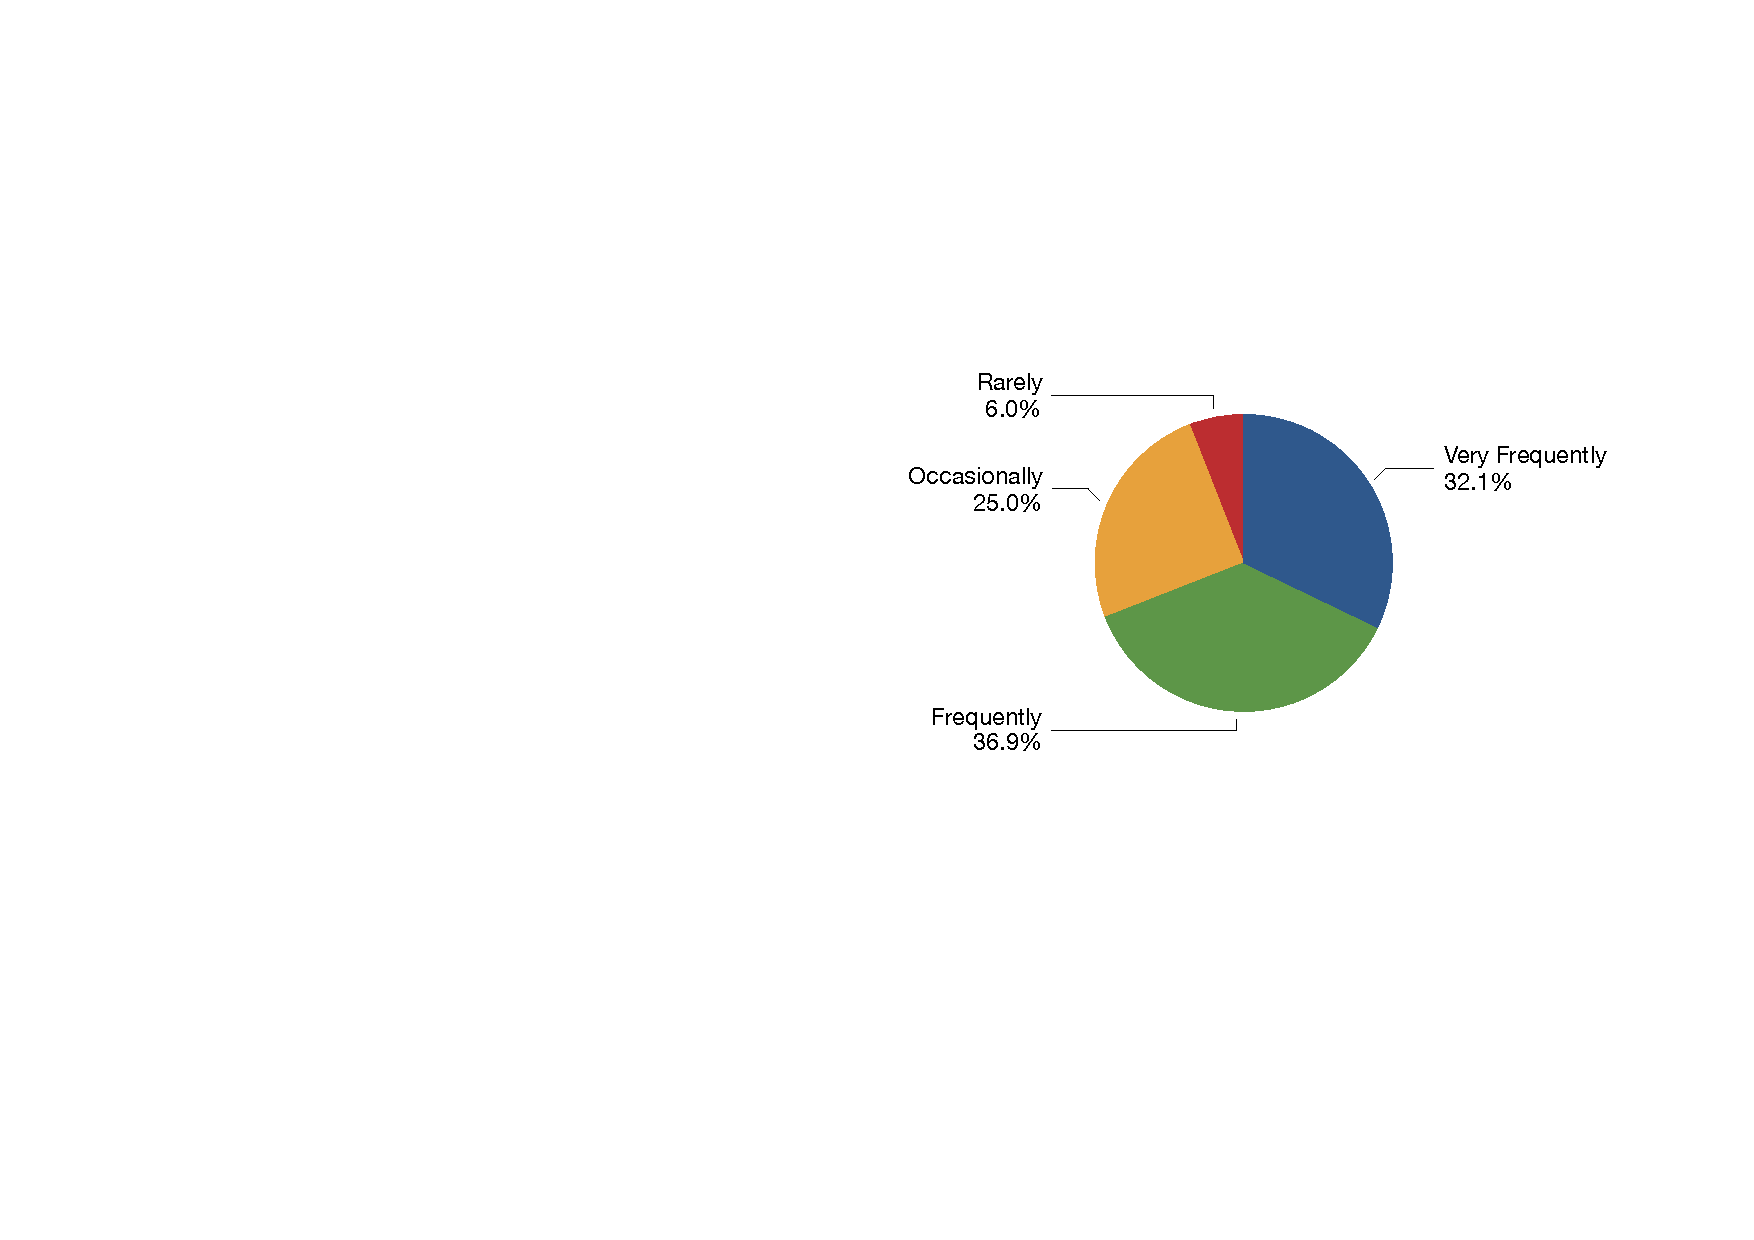
\includegraphics[width=0.9\linewidth]{survey_answer_frequency_with_code_2}
		\caption{Group 2}
		\label{fig:survey_answer_frequency_with_code_2}
	\end{subfigure}
	\caption{Frequency of answering questions with code snippet(s)}
	\label{fig:survey_answer_frequency_with_code}
\end{figure}

\subsubsection*{RQ1: Where are the code snippets in Stack Overflow answers from?} 

To answer this research question, we ask the participants of the original
sources for their code examples. We provided six options (allowing more than one answer)
including \textit{I copied them from my own personal projects}, \textit{I copied
	them from my company's projects}, \textit{I copied them from open source
	projects}, \textit{I wrote the new code from scratch}, \textit{I copied the code
	from the question and modify it for the answer}, and \textit{Others}. From the
answers (Figure~\ref{fig:survey_snippet_source}), Stack Overflow answerers
in Group 1 mainly write new code from scratch (112) or copy from the code snippets in question
and modify it for the answer (108), followed by from their personal
projects (101), open source projects (73), other sources (57), and company projects (46). 
For Group 2, the most selected option is also writing code from scratch (83), followed by copying
from personal projects and modifying from the question (77), copying from open source projects (56),
copying from other sources (40), and copying from company projects (31).

\begin{figure*}
	\begin{subfigure}{.5\textwidth}
		\centering
		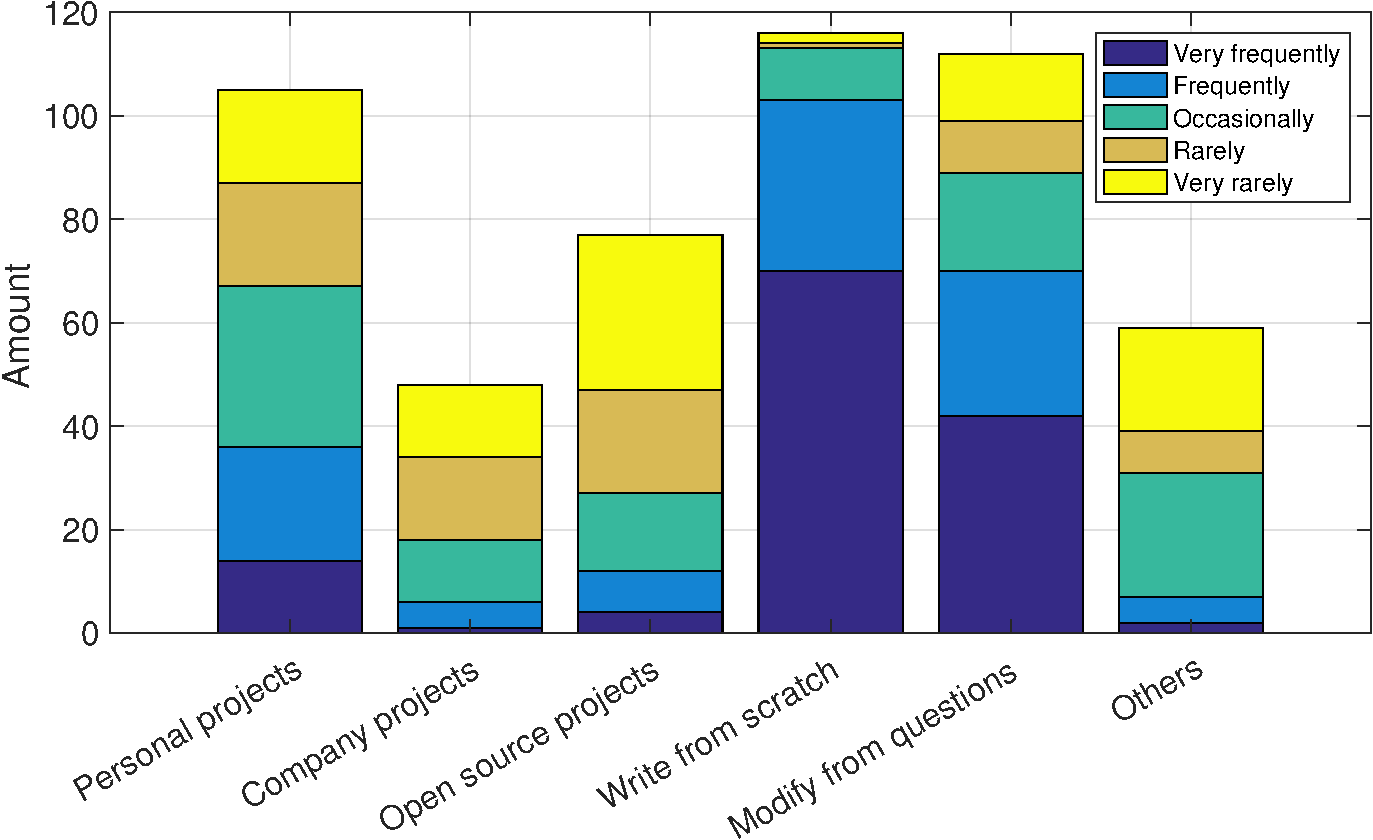
\includegraphics[width=.9\linewidth]{survey_snippet_source_1}
		\caption{Group 1}
		\label{fig:survey_snippet_source_1}
	\end{subfigure}%
	\begin{subfigure}{.5\textwidth}
		\centering
		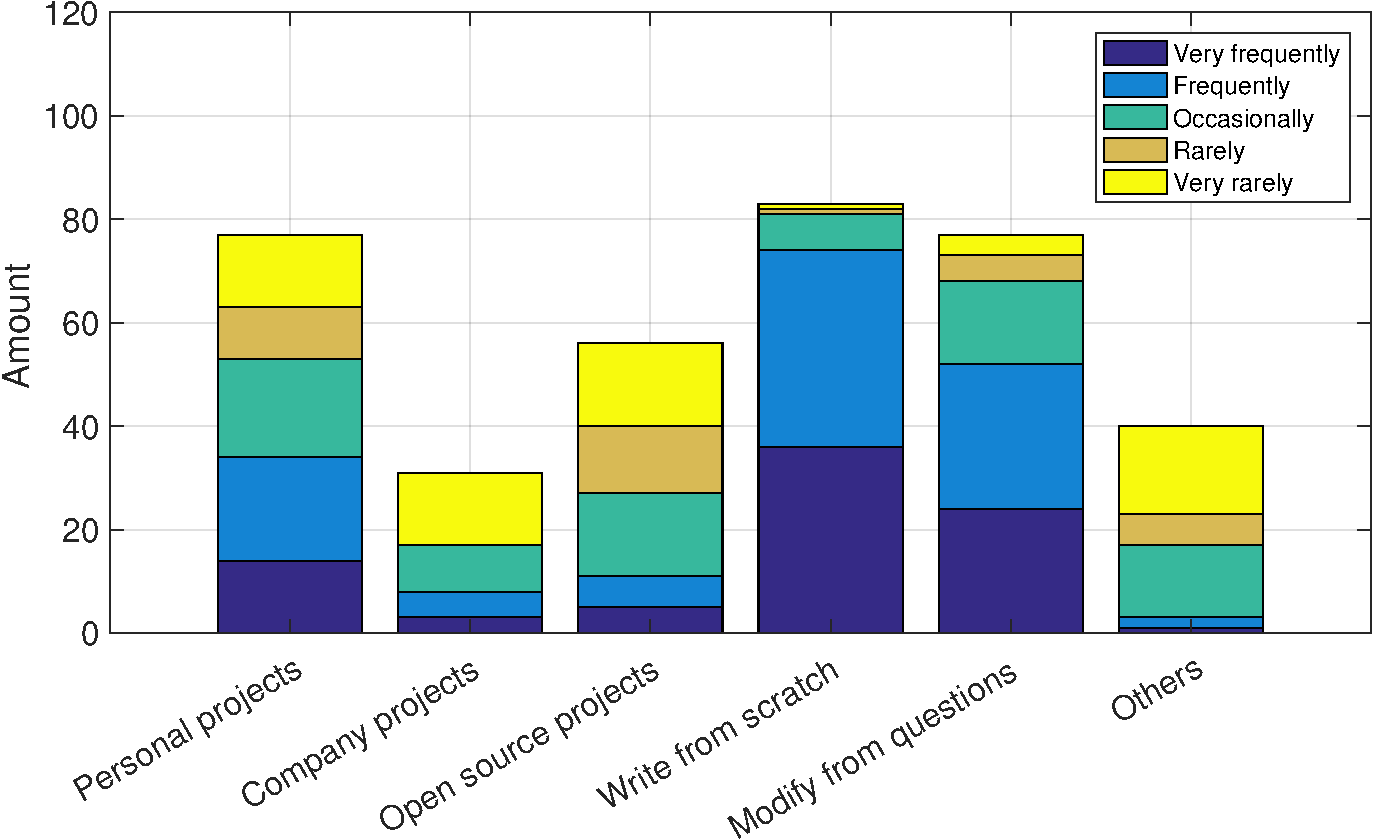
\includegraphics[width=.9\linewidth]{survey_snippet_source_2}
		\caption{Group 2}
		\label{fig:survey_snippet_source_2}
	\end{subfigure}
	\caption{Sources of code snippets in Stack Overflow answers}
	\label{fig:survey_snippet_source}
\end{figure*}

\vspace{0.5cm}
\noindent\fbox{%
	\parbox[c][1.5cm]{0.98\textwidth}{%
		\textit{For RQ 1, we found almost every answerer writes the new code from scratch or modifies from the code in question most of the time. Other less popular choices include copying code from their personal projects, and open source projects. Company projects are the least popular choice.}
	}%
}
\vspace{0.5cm}

\subsubsection*{RQ2: Are Stack Overflow answerers aware of outdated code in their answers?}

Roughly half of the top answerers on Stack Overflow
are aware of outdated code in their answers. We found that 72.3\% of Stack Overflow answerers in Group 1 have been notified of
outdated code in at least one of their answers (see Figure~\ref{fig:survey_outdated}). The ratio drops to 57.1\% in
Group 2. 

\begin{figure}
	\centering
	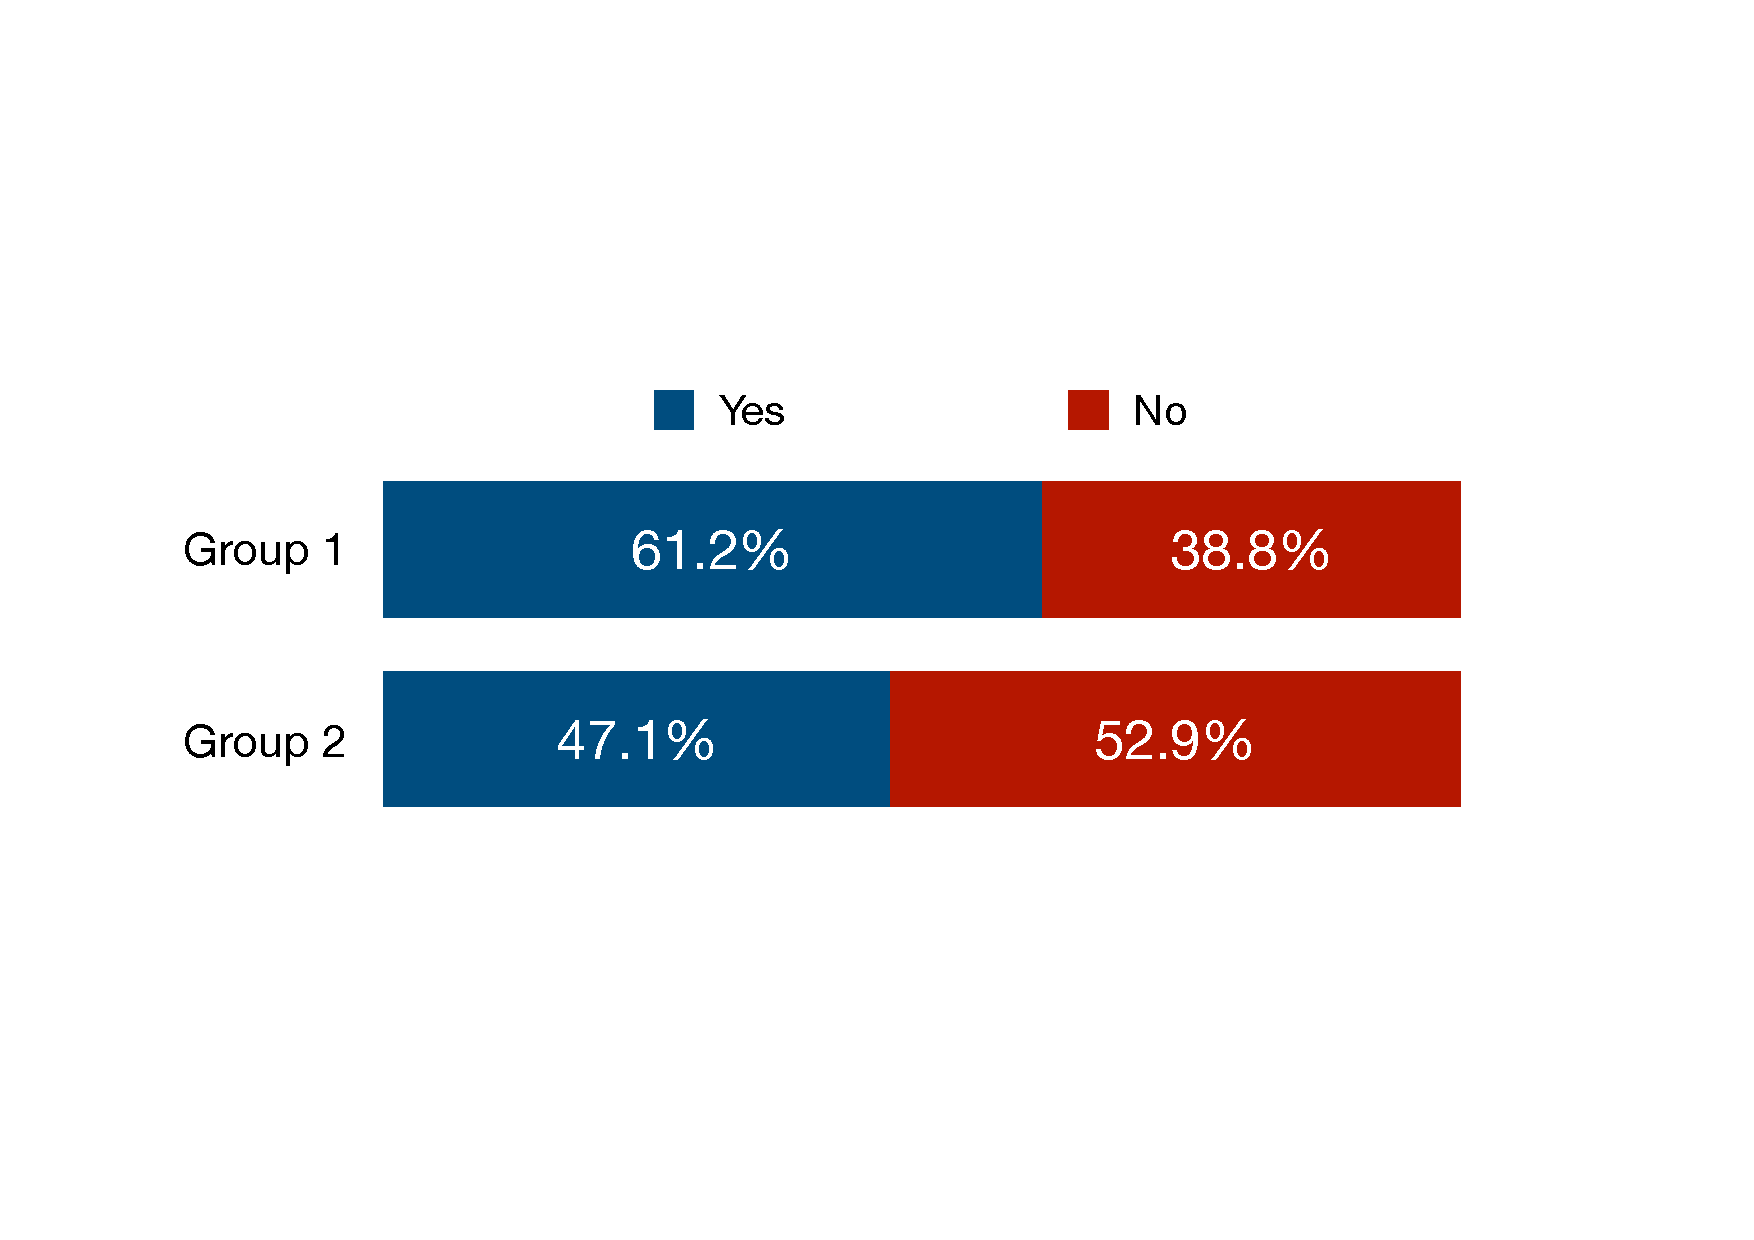
\includegraphics[width=.5\linewidth]{survey_outdated}
	\caption{Percentage of answerers who are notified of outdated code in their Stack Overflow answers.}
	\label{fig:survey_outdated}
\end{figure}

\begin{figure}
	\begin{subfigure}{.5\textwidth}
		\centering
		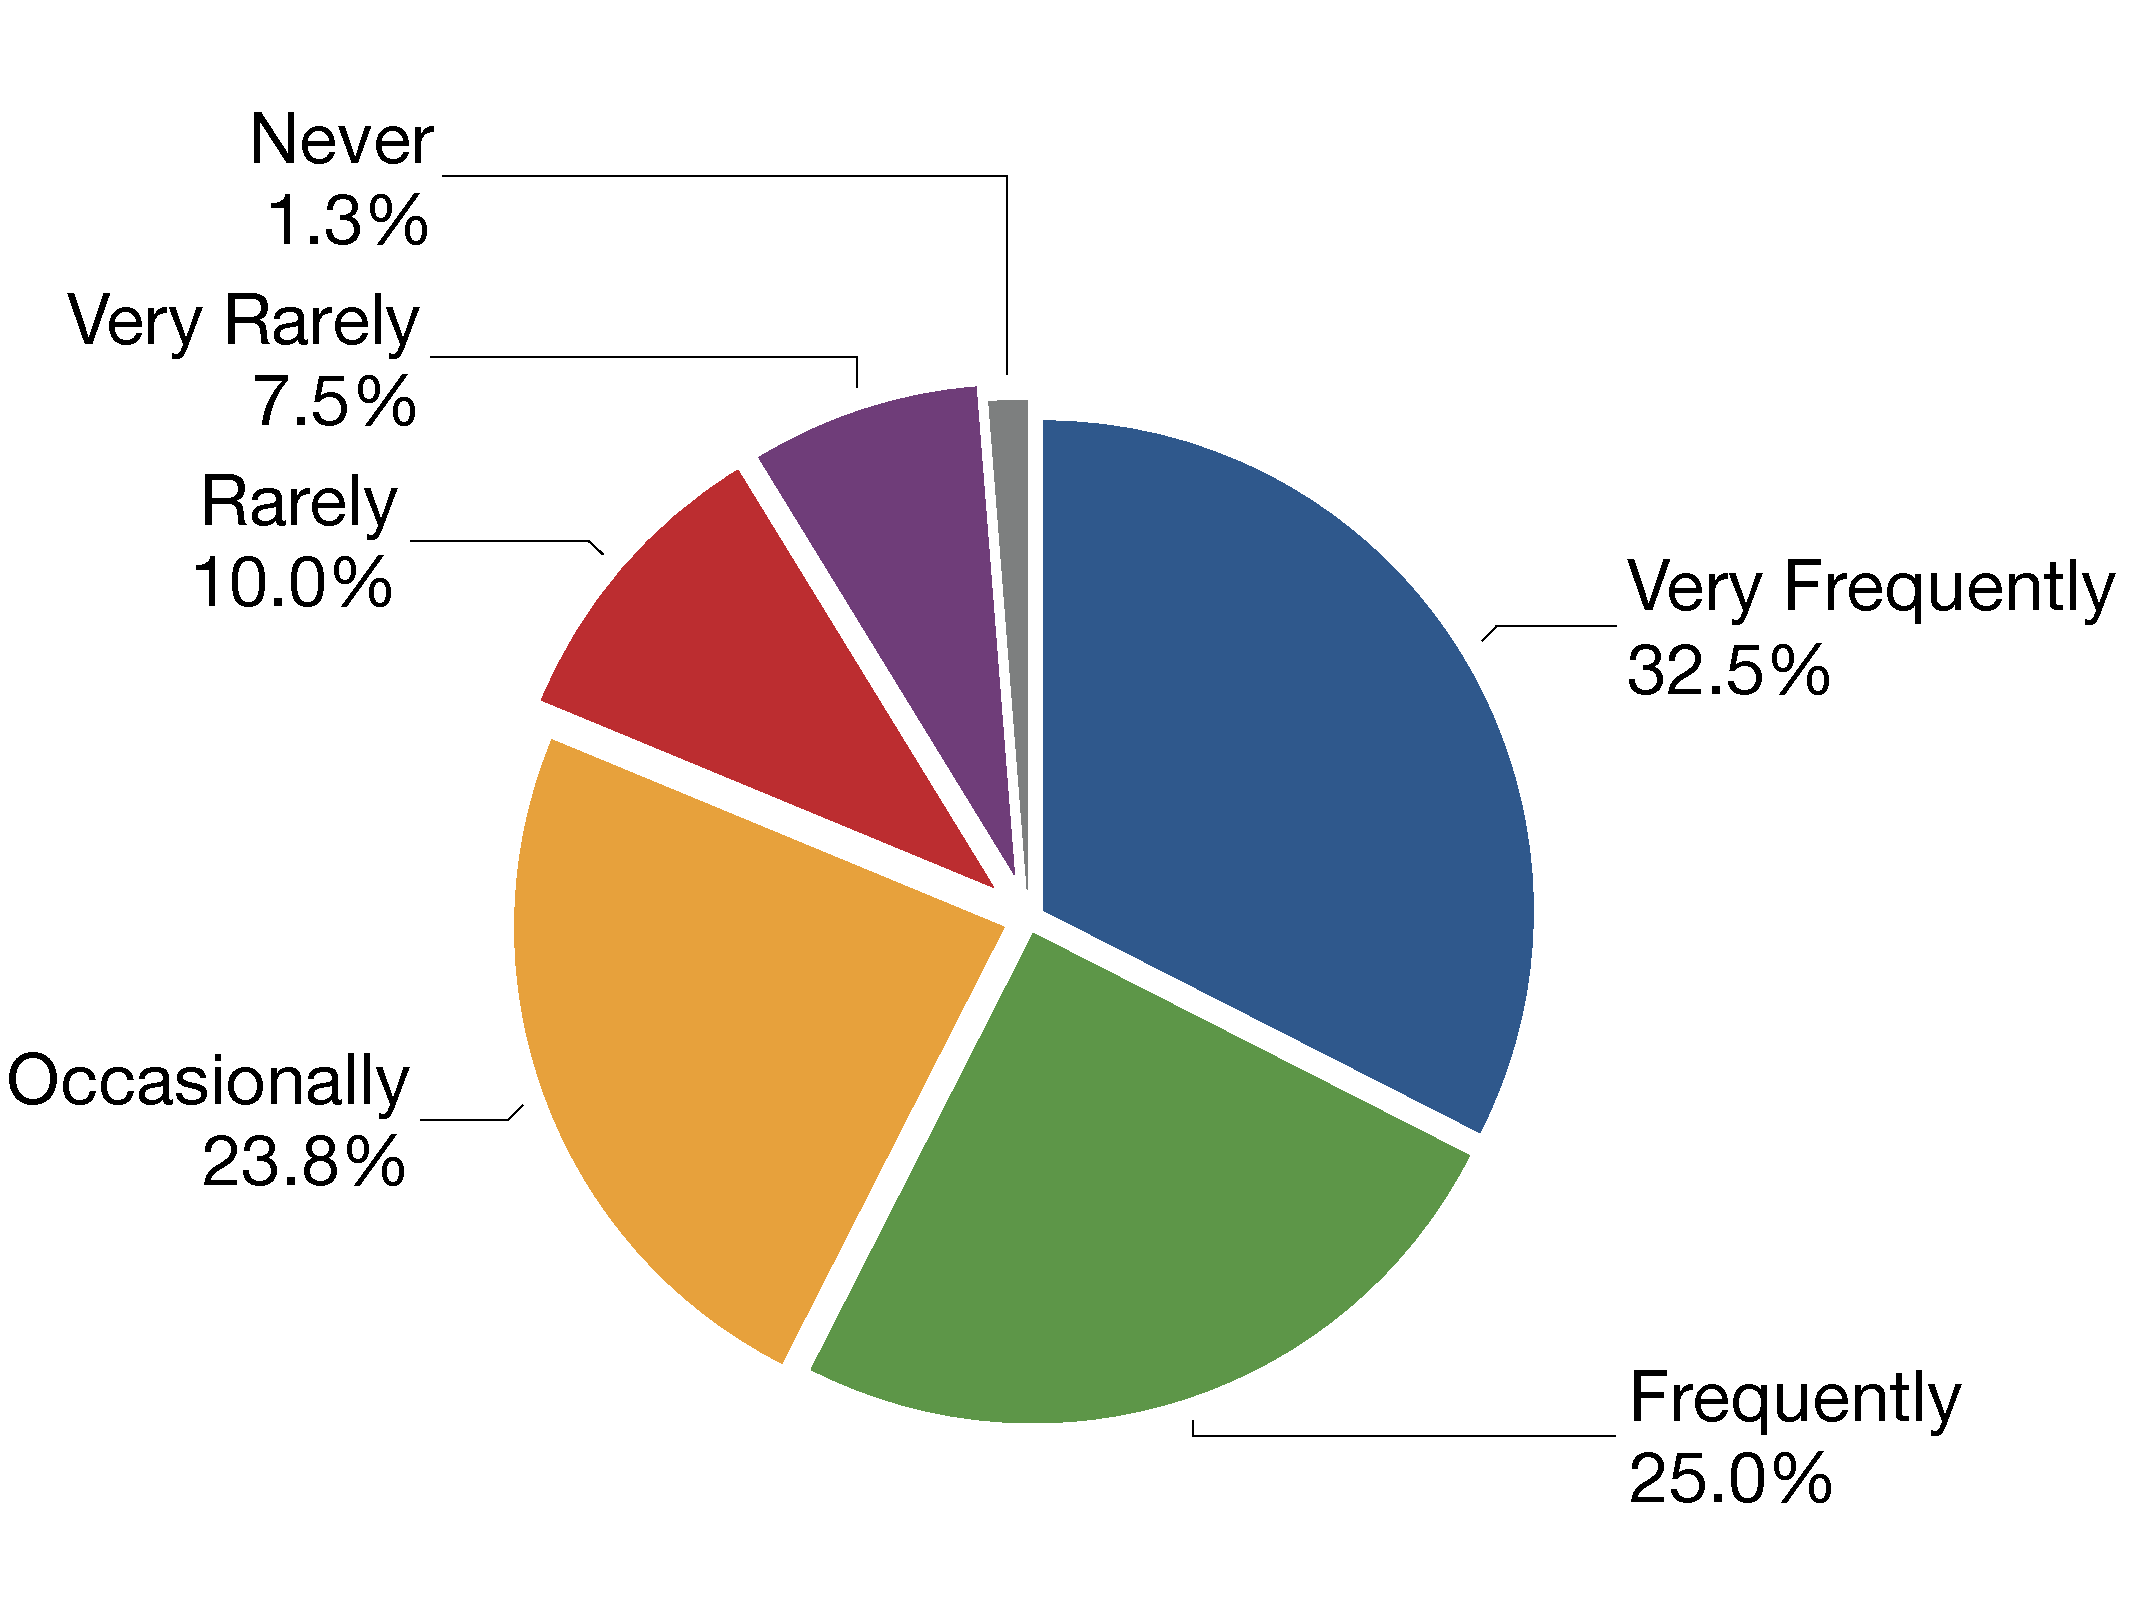
\includegraphics[width=.8\linewidth]{survey_outdated_fix_1}
		\caption{Group 1}
		\label{fig:survey_outdated_fix_1}
	\end{subfigure}%
	\begin{subfigure}{.5\textwidth}
		\centering
		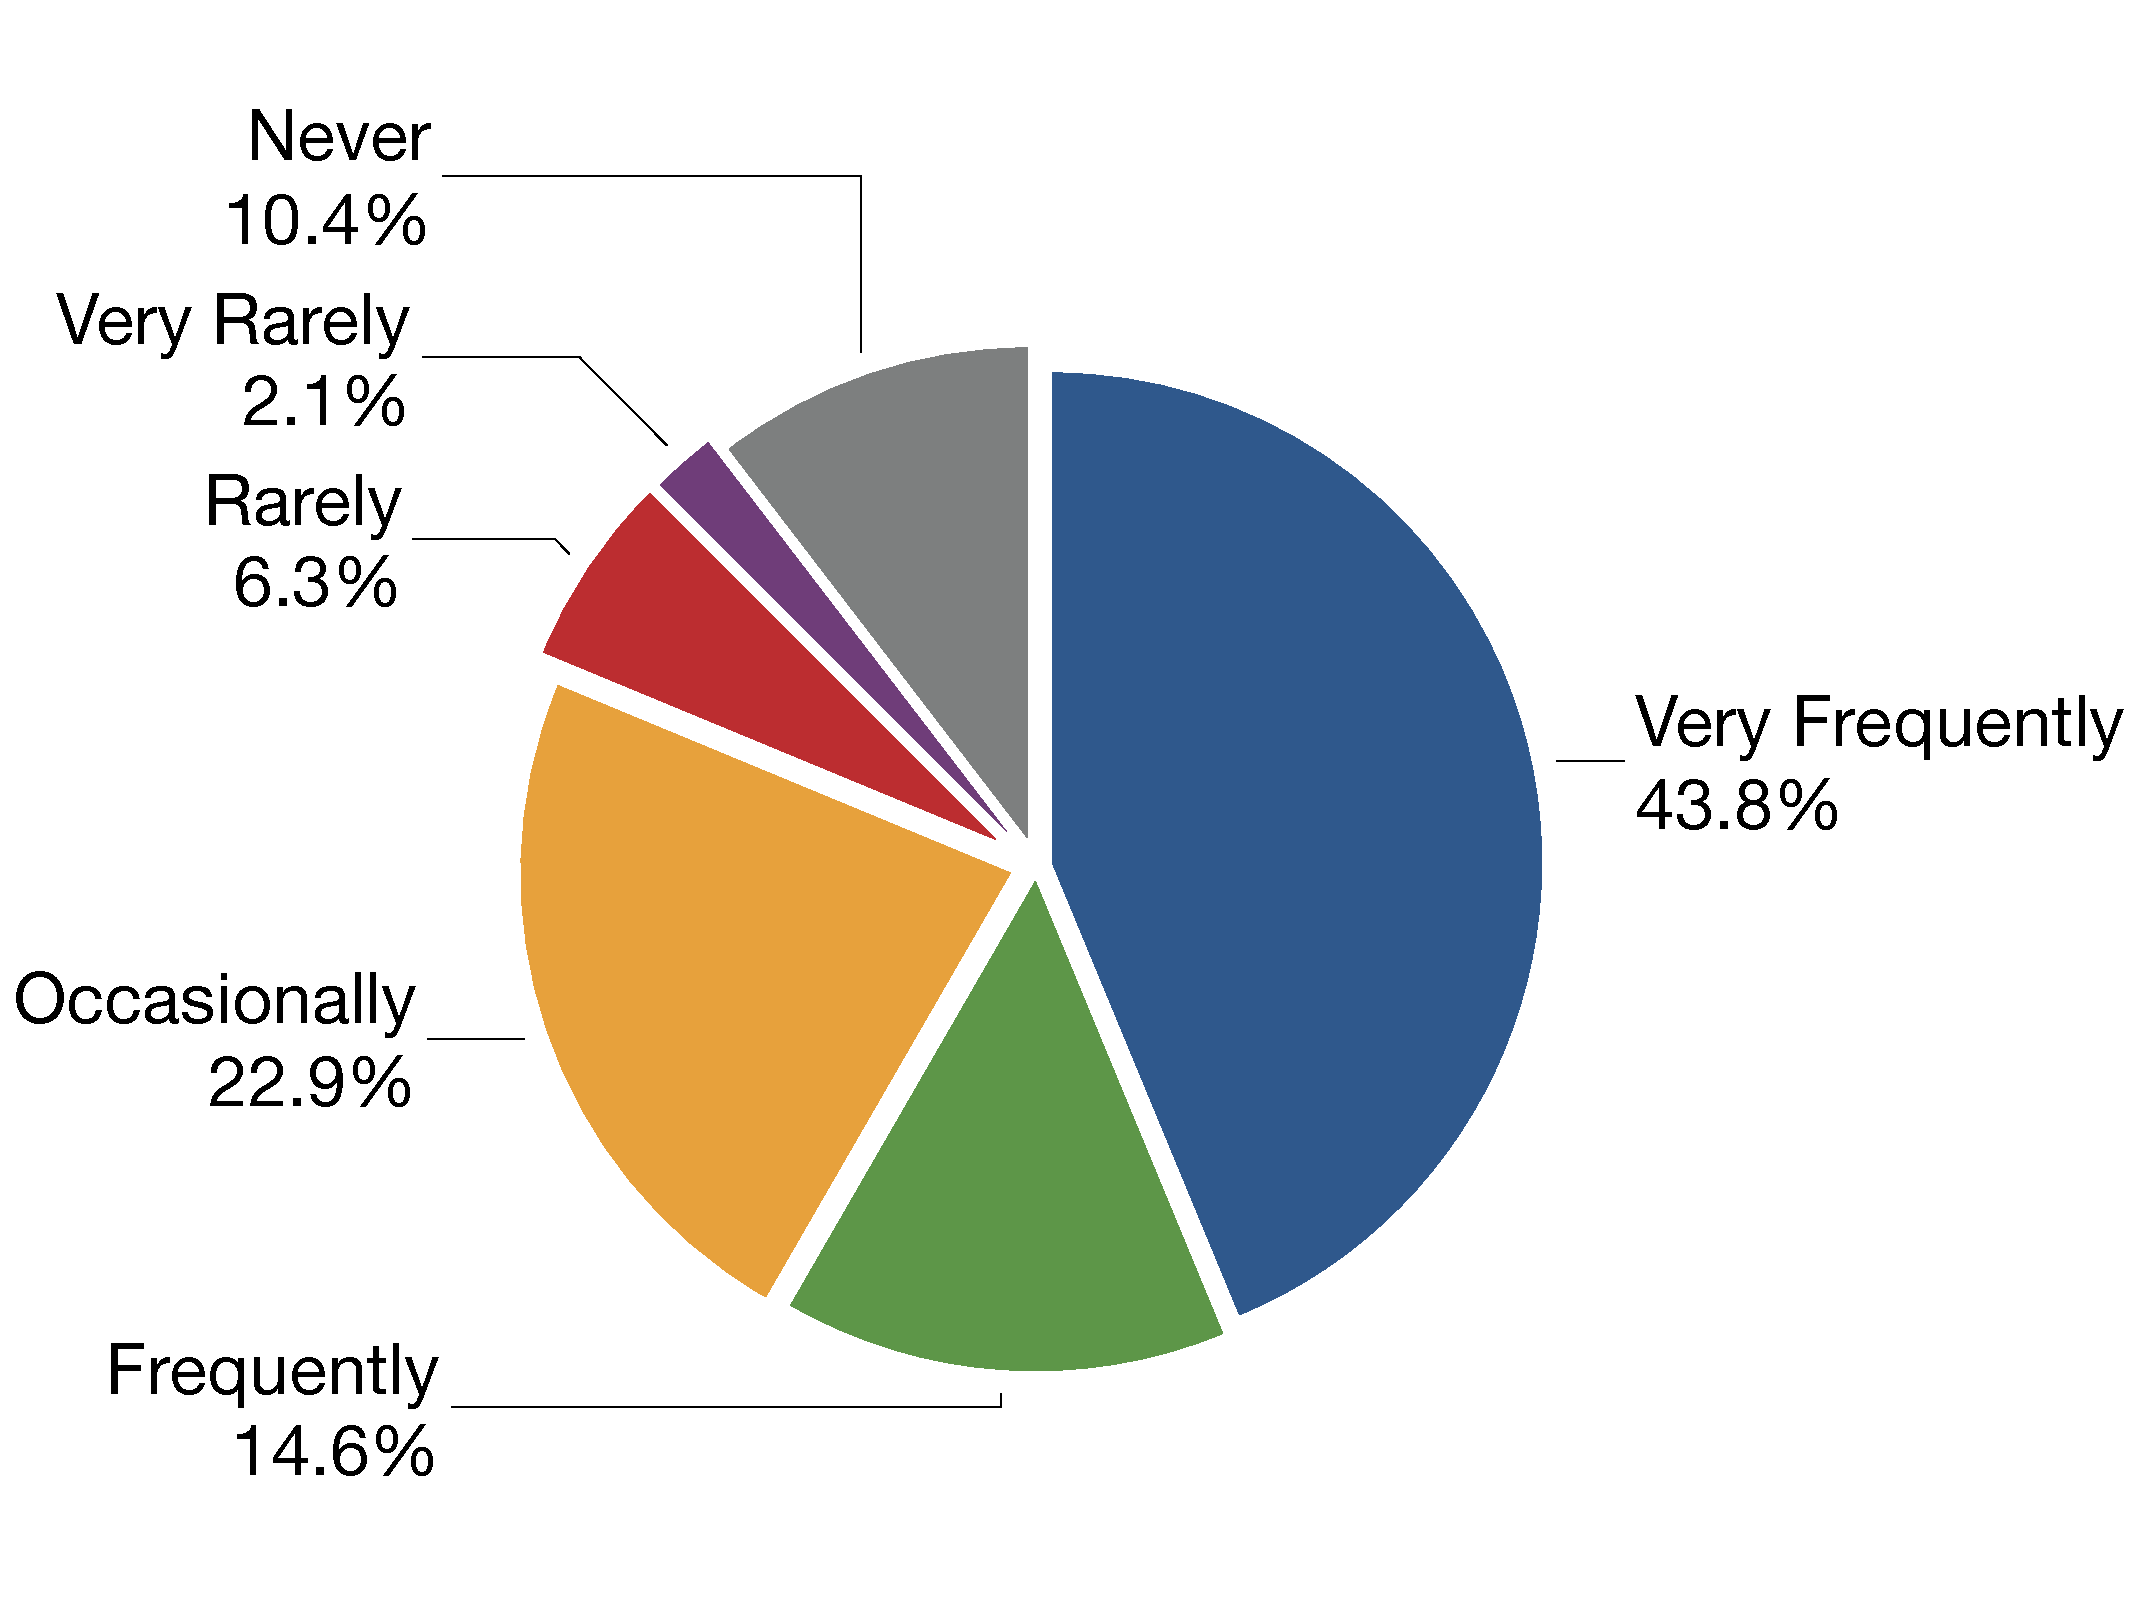
\includegraphics[width=.8\linewidth]{survey_outdated_fix_2}
		\caption{Group 2}
		\label{fig:survey_outdated_fix_2}
	\end{subfigure}
	\caption{Frequency of the answerers fixing their outdated code.}
	\label{fig:survey_outdated_fix}
\end{figure}

We then asked the participants who have been notified of their outdated code
(81 and 48 participants from Group 1 and 2 respectively) a
follow-up questions \textit{``how frequently did you fix your outdated code on Stack
Overflow?''} The answers, depicted in Figure~\ref{fig:survey_outdated_fix}, show that
more than half of them frequently fix the outdated code snippets. However, there
are 19.8\% and 18.8\% of the answerers in Groups 1 and 2 who rarely or never fix their code.

\vspace{0.5cm}
\noindent\fbox{%
	\parbox[c][1.2cm]{0.98\textwidth}{%
		\textit{For RQ 2, we found that the majority of Stack Overflow answerers are aware of outdated code in their answers and fixed them. Nonetheless, there are approximately 19\% of the answerers who rarely or never fix their outdated code.}
	}%
}
\vspace{0.5cm}

\subsubsection*{RQ3: Are Stack Overflow answerers aware of software licensing conflicts caused by code snippets in their answers?} 

As shown in Figure~\ref{fig:survey_license_known}, more than half of the
answerers in both groups (63.4\% and 61.9\% respectively) are aware that Stack
Overflow apply Creative Commons Attribution-ShareAlike 3.0 Unported (CC BY-SA
3.0) to content in the posts, including code snippets, while the rest of 36.6\%
and 38.1\% are not. 

\begin{figure}
	\begin{subfigure}{.5\textwidth}
		\centering
		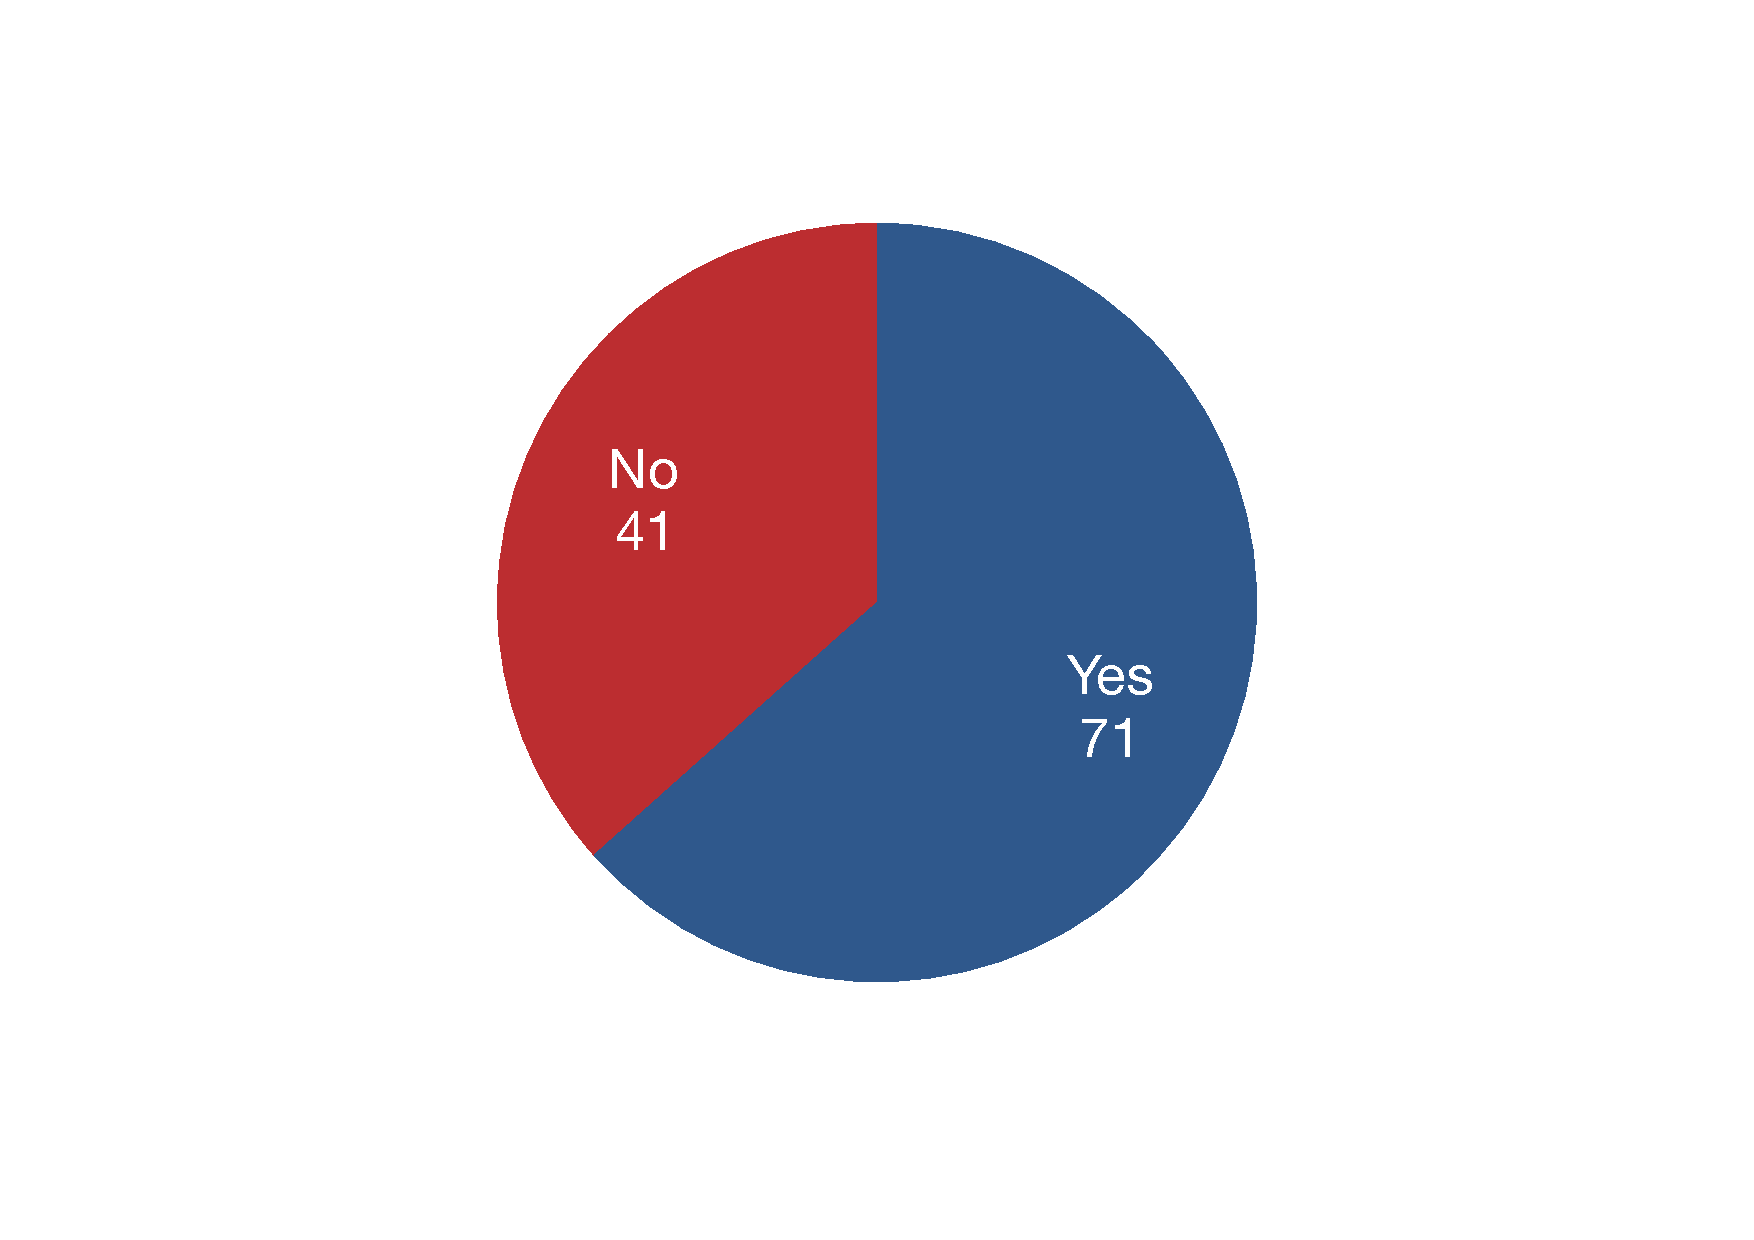
\includegraphics[width=.4\linewidth]{survey_license_known_1}
		\caption{Group 1}
		\label{fig:survey_license_known_1}
	\end{subfigure}%
	\begin{subfigure}{.5\textwidth}
		\centering
		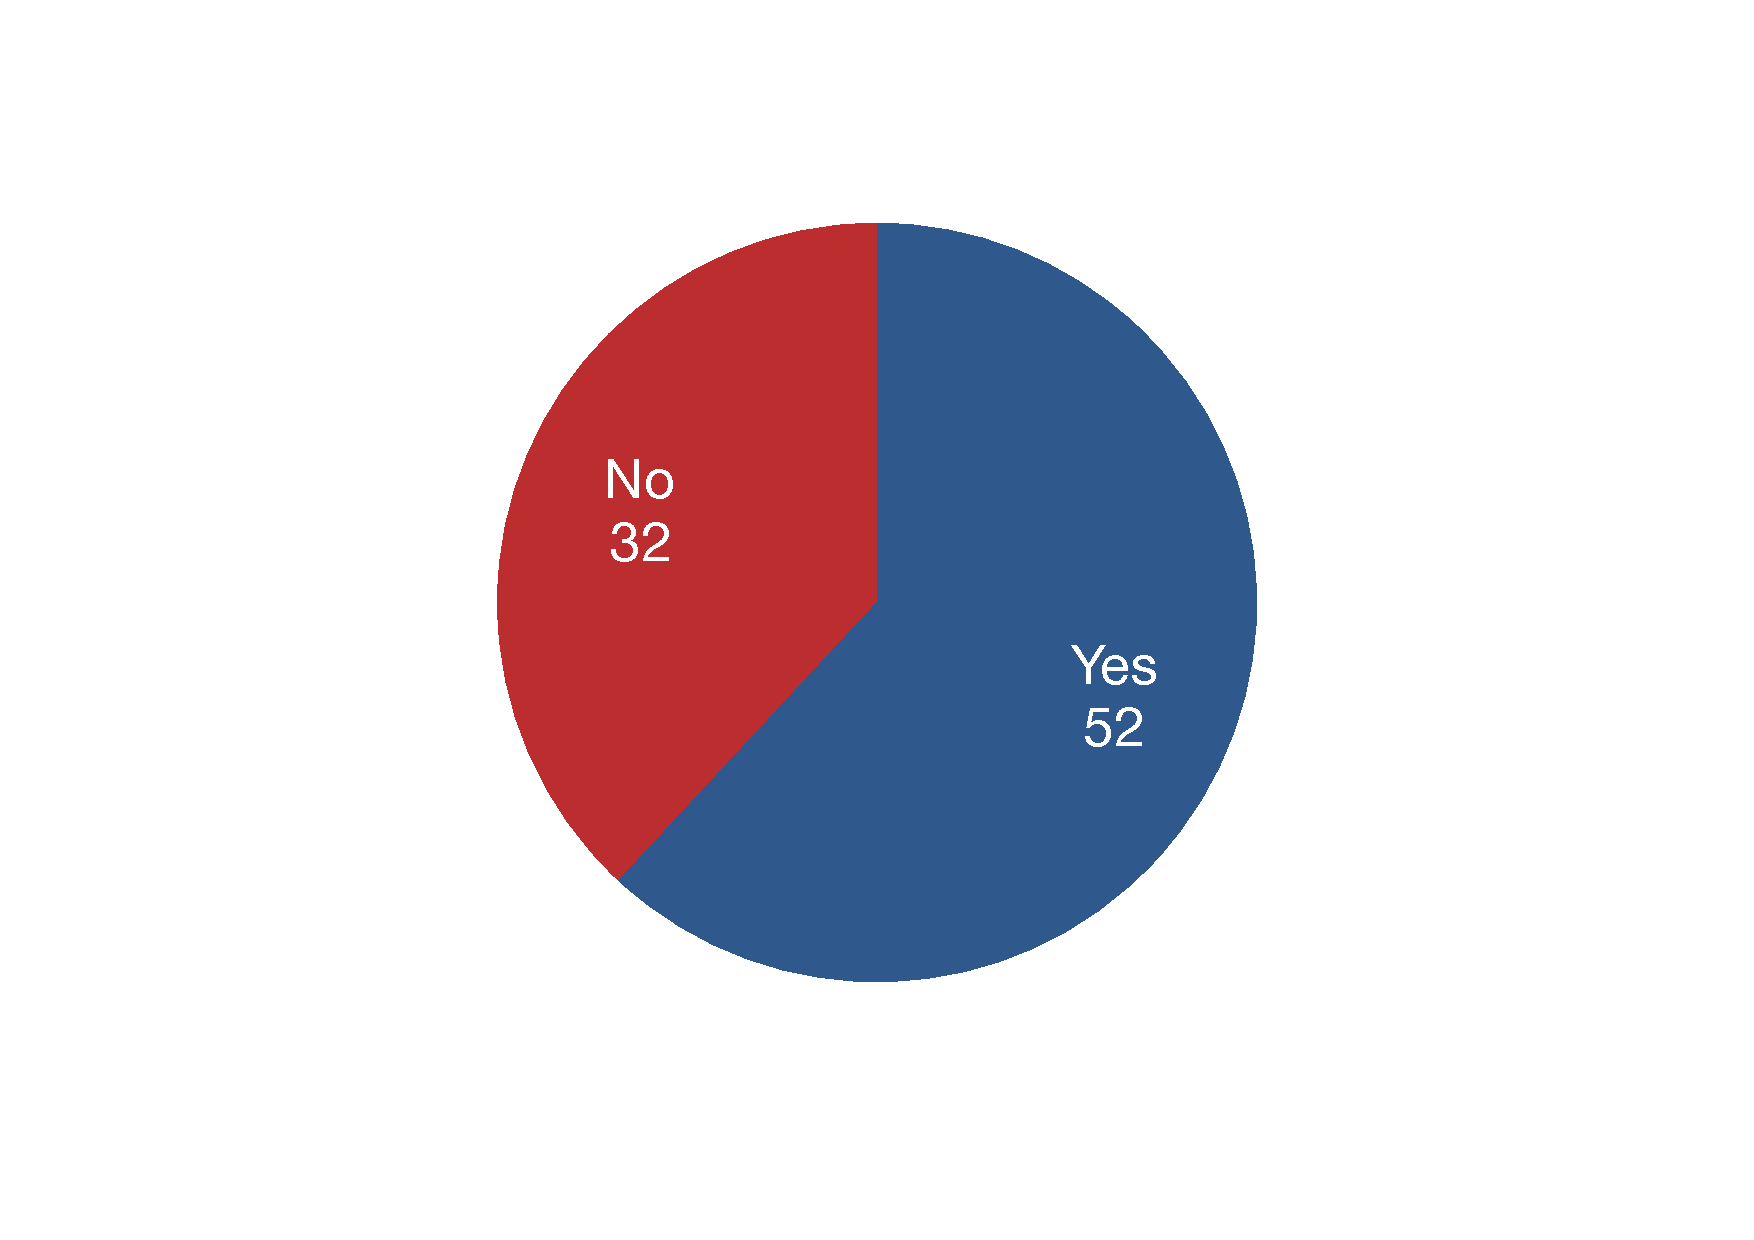
\includegraphics[width=.4\linewidth]{survey_license_known_2}
		\caption{Group 2}
		\label{fig:survey_license_known_2}
	\end{subfigure}
	\caption{Awareness of answerers to Stack Overflow CC BY-SA 3.0 license}
	\label{fig:survey_license_known}
\end{figure}

In addition, we found that almost every answerer in both groups (98\% and
99\% respectively) do not include license statement in their code snippets
(numbers are shown in Figure~\ref{fig:survey_license}). Some of the participants
gave more information regarding this question in the open comment question and
we summarised them into three groups as follows. First, some answerers chose to post only their
own code or code that was adapted from the question. They are hence
automatically subjected to CC BY-SA 3.0. Second, they copied code from company
or open source projects that they knew were permitted to be publicly
distributed. Third, some answerers believe that code snippets in their answers
are too small to claim any intellectual property on them and fall under fair
use~\citep{fairuse}.

\begin{figure}
	\begin{subfigure}{.5\textwidth}
		\centering
		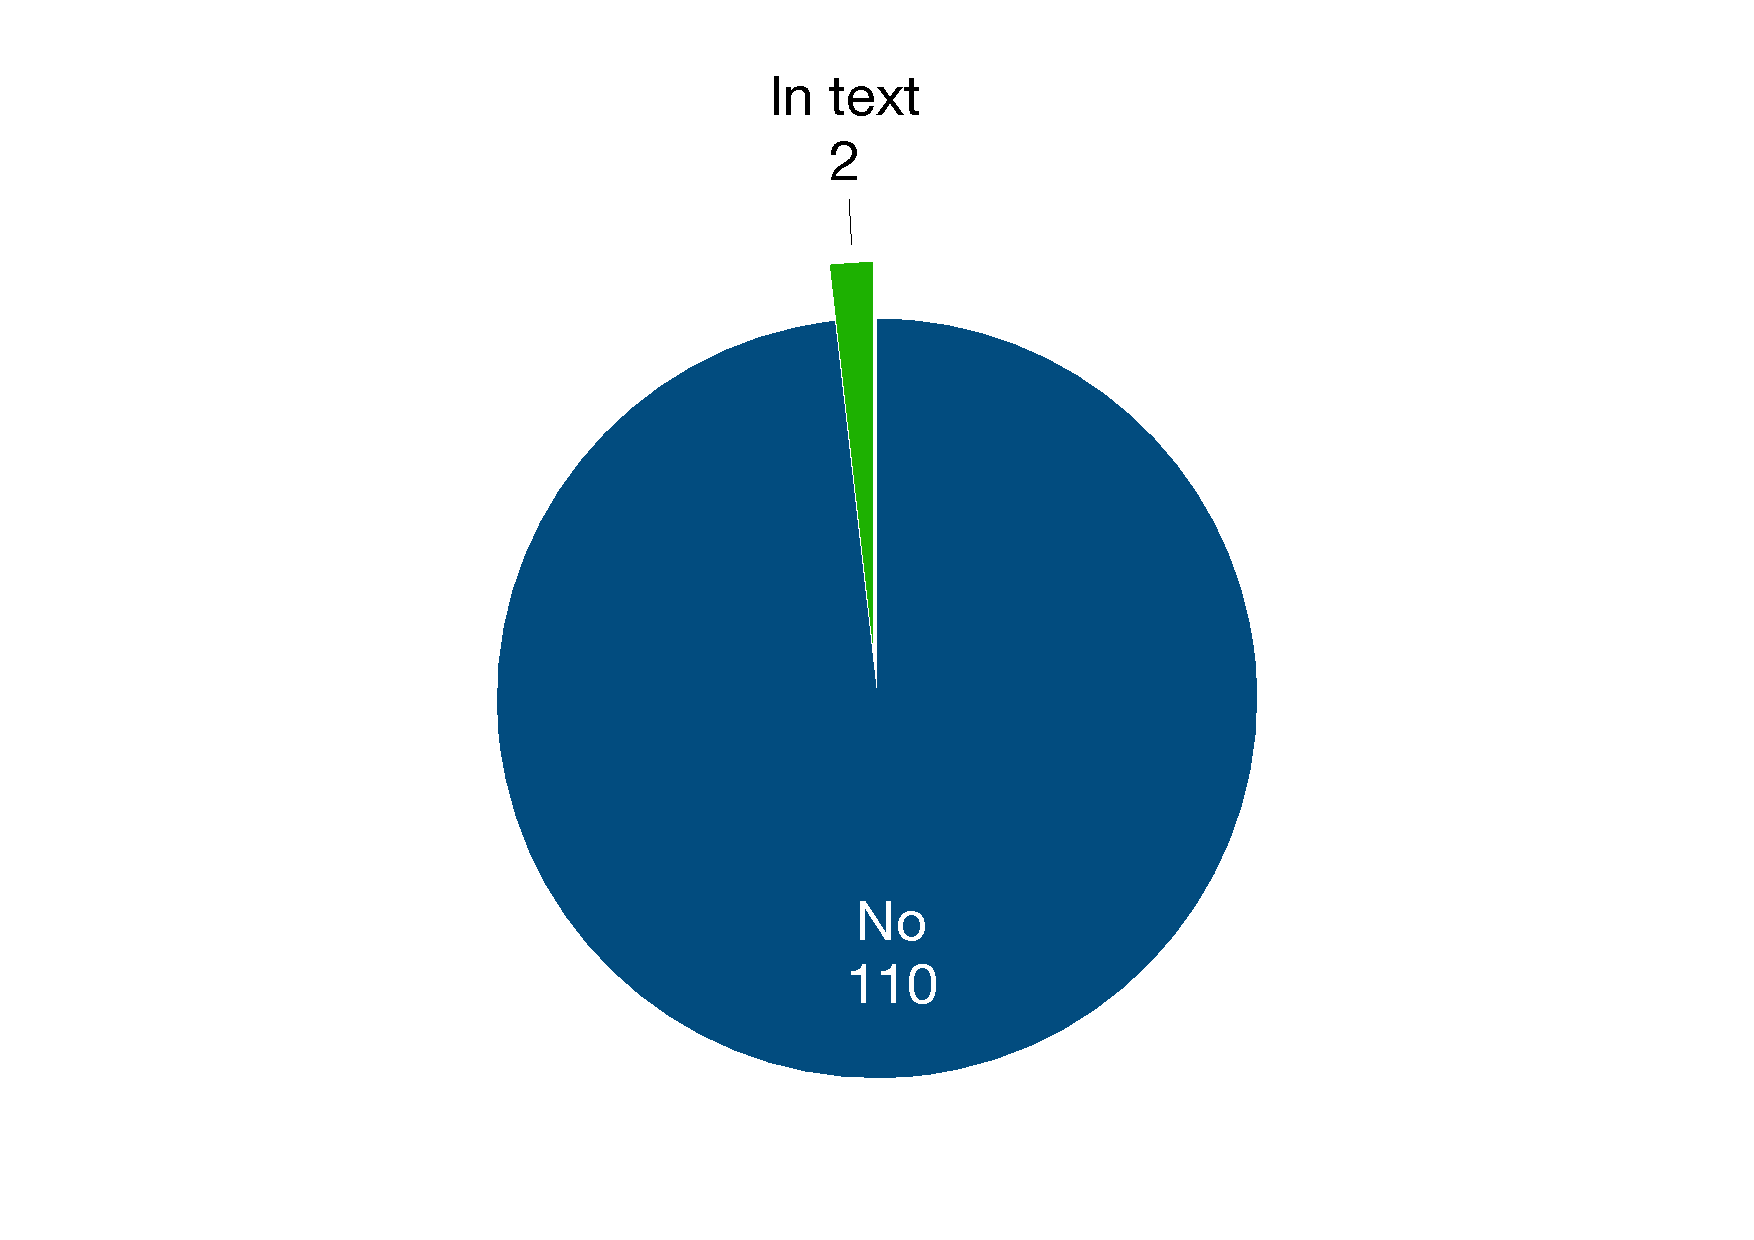
\includegraphics[width=.4\linewidth]{survey_license_1}
		\caption{Group 1}
		\label{fig:survey_license_1}
	\end{subfigure}%
	\begin{subfigure}{.5\textwidth}
		\centering
		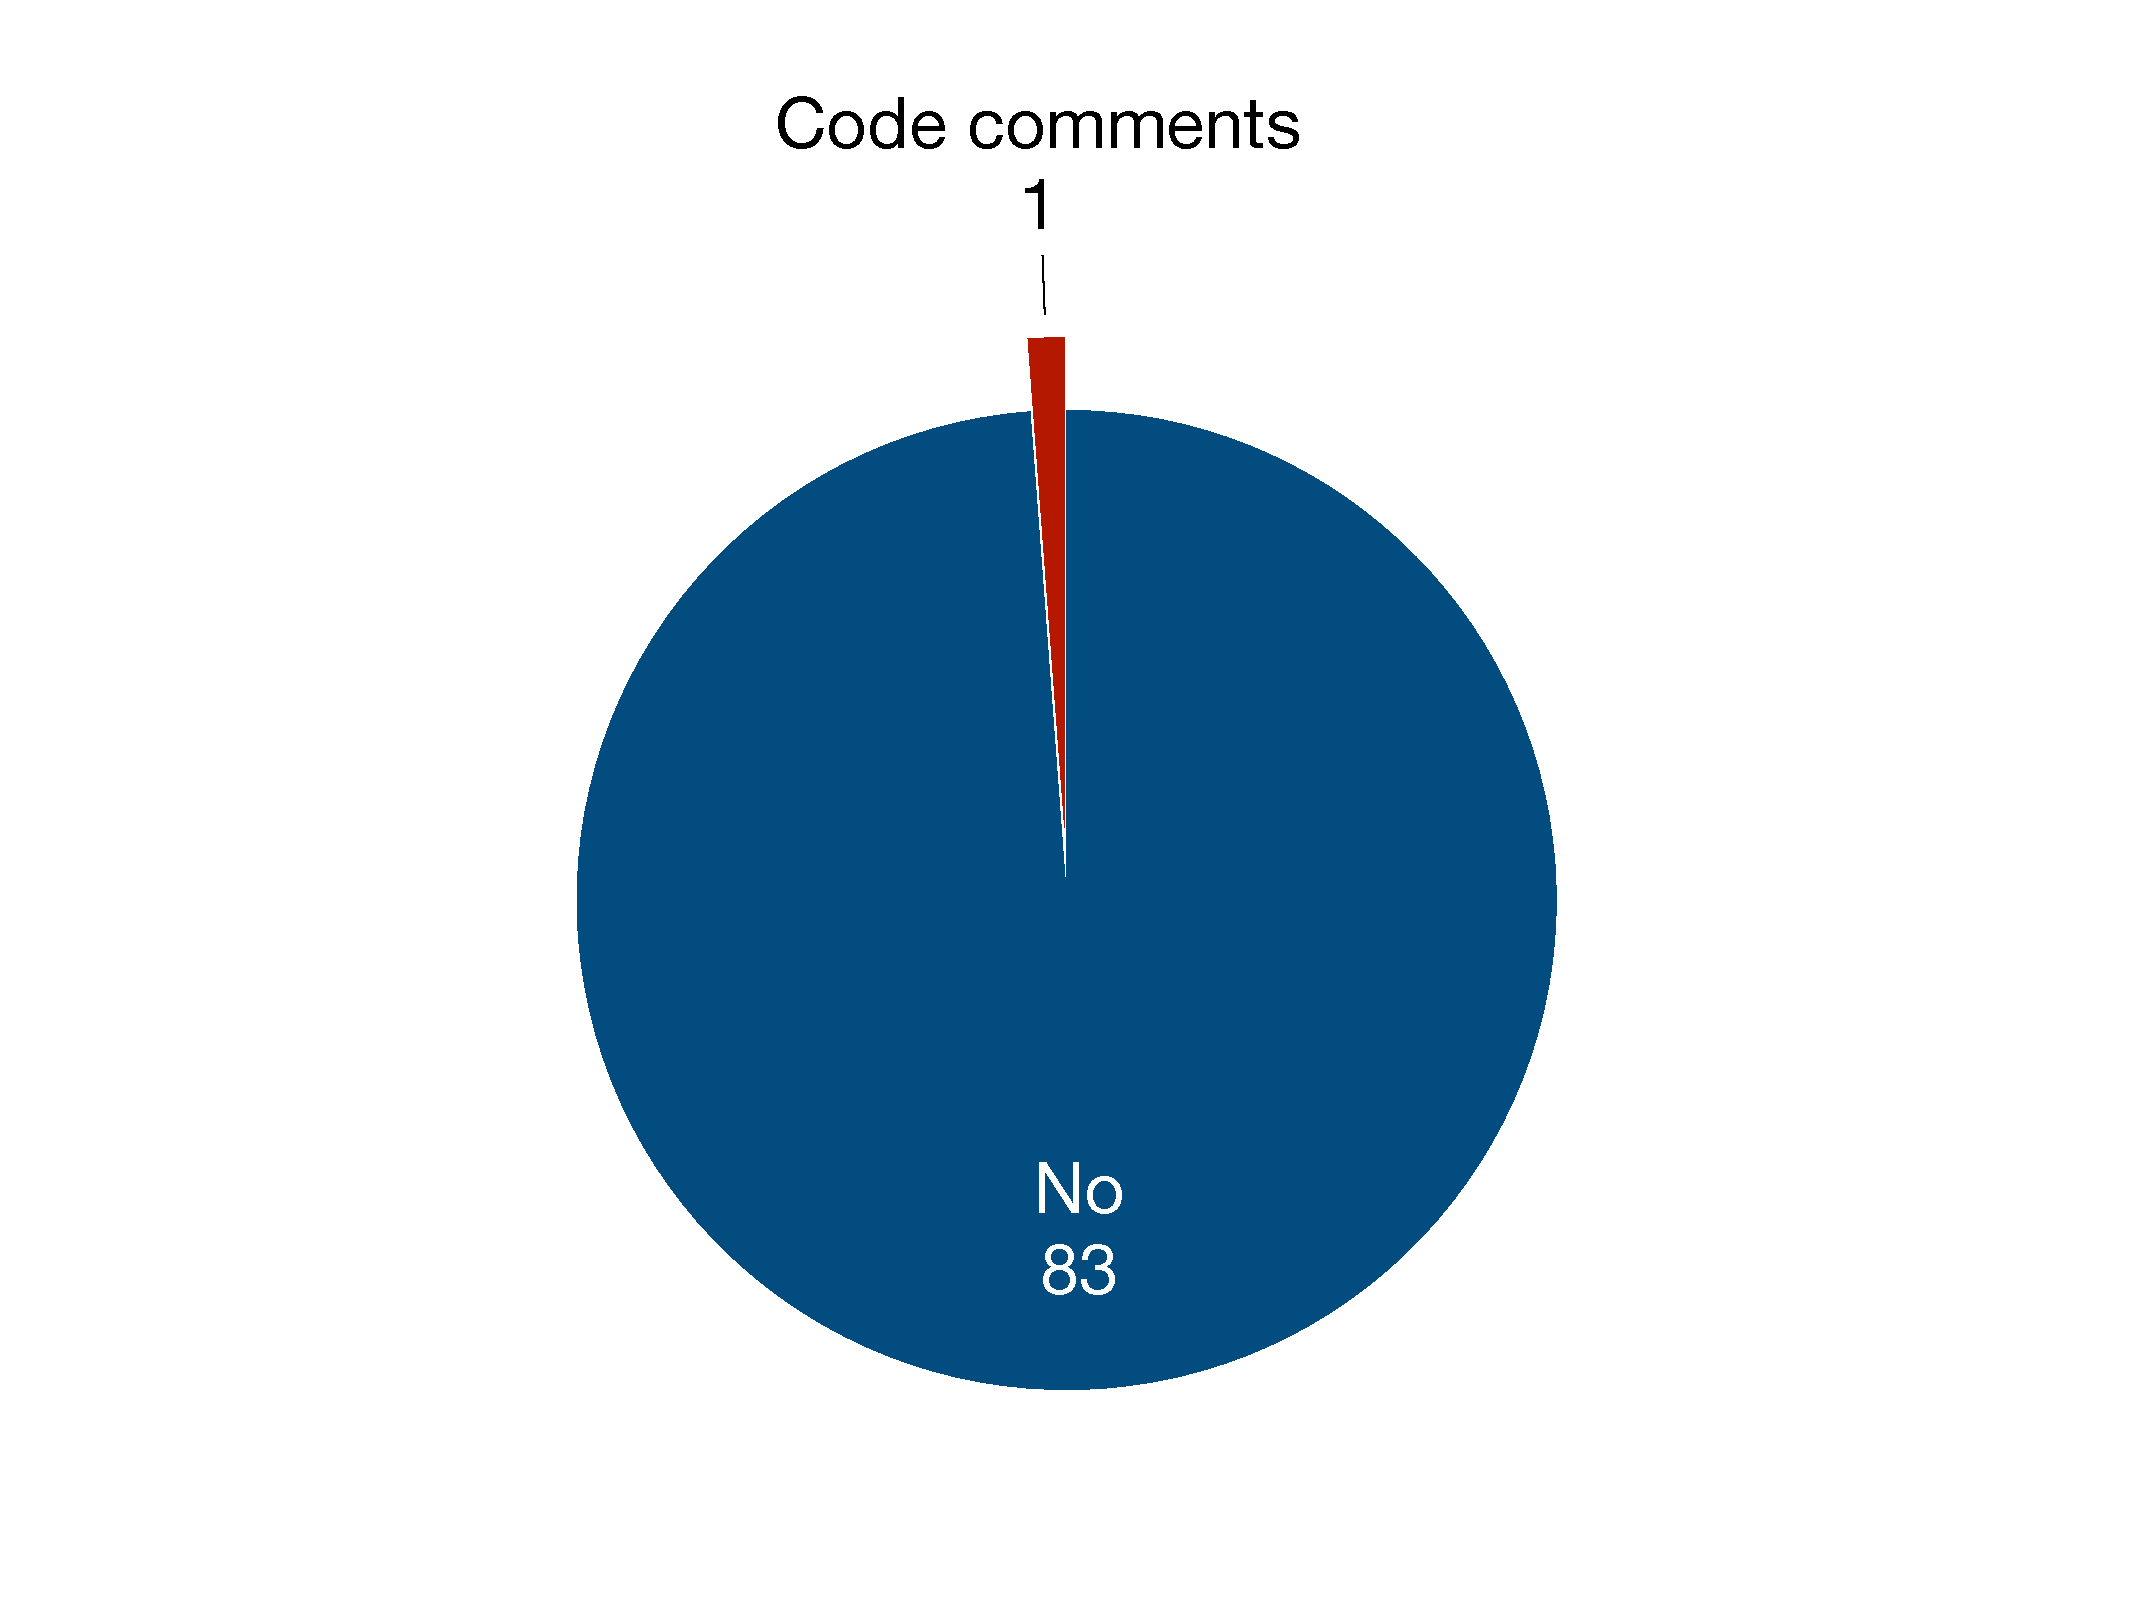
\includegraphics[width=.4\linewidth]{survey_license_2}
		\caption{Group 2}
		\label{fig:survey_license_2}
	\end{subfigure}
	\caption{Software license in Stack Overflow code snippets.}
	\label{fig:survey_license}
\end{figure}

While nobody explicitly includes a software license in their snippets,
many users include a statement on their profile page that states all their
answers are under a certain license. For example, \textit{All code posted by me on
	Stack Overflow should be considered public domain without copyright. For
	countries where public domain is not applicable, I hereby grant everyone the
	right to modify, use and redistribute any code posted by me on Stack Overflow
	for any purpose. It is provided "as-is" without warranty of any kind.}  Many
users either declare their snippets to be public domain, or they grant
additional licenses, e.g. Apache 2.0 or MIT/Expat.

\begin{figure}
	\begin{subfigure}{.5\textwidth}
		\centering
		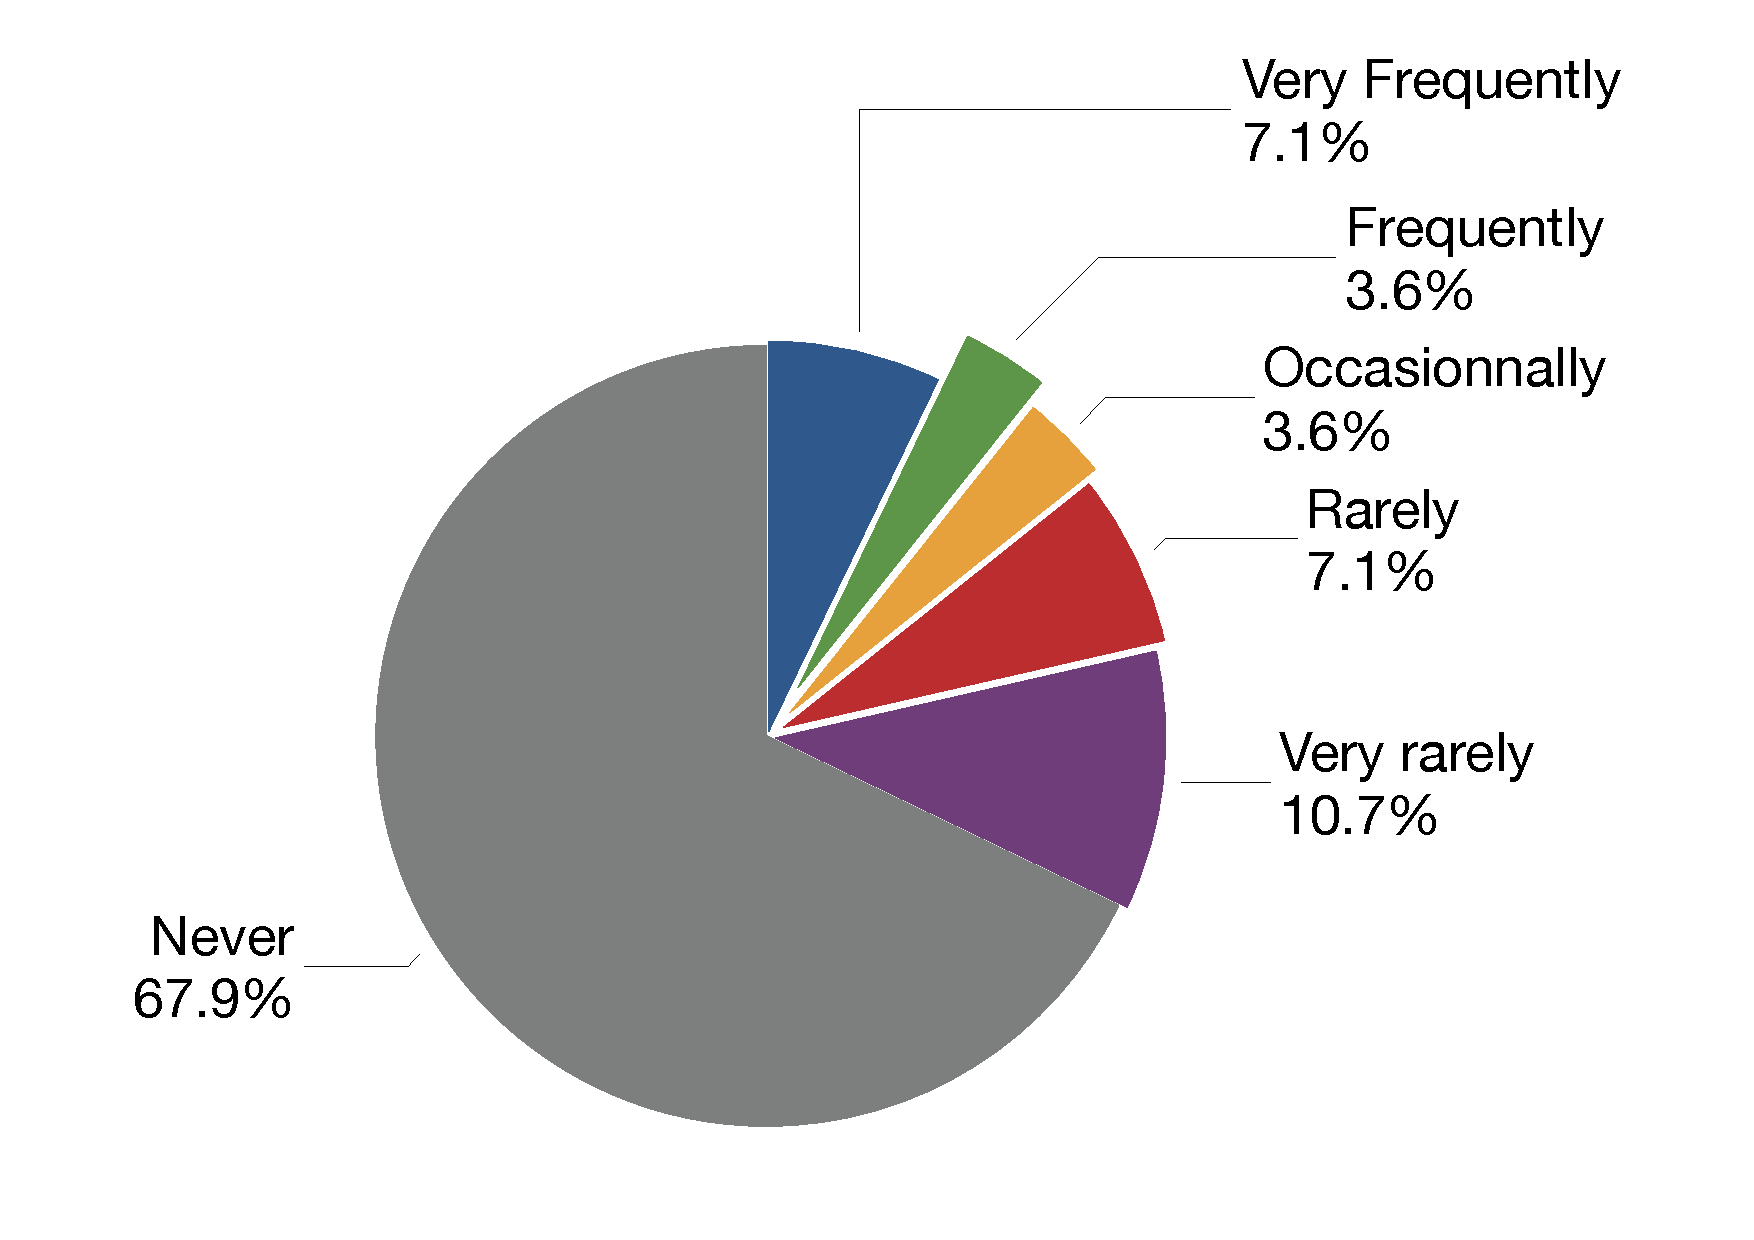
\includegraphics[width=.75\linewidth]{survey_license_check_1}
		\caption{Group 1}
		\label{fig:survey_license_check_1}
	\end{subfigure}%
	\begin{subfigure}{.5\textwidth}
		\centering
		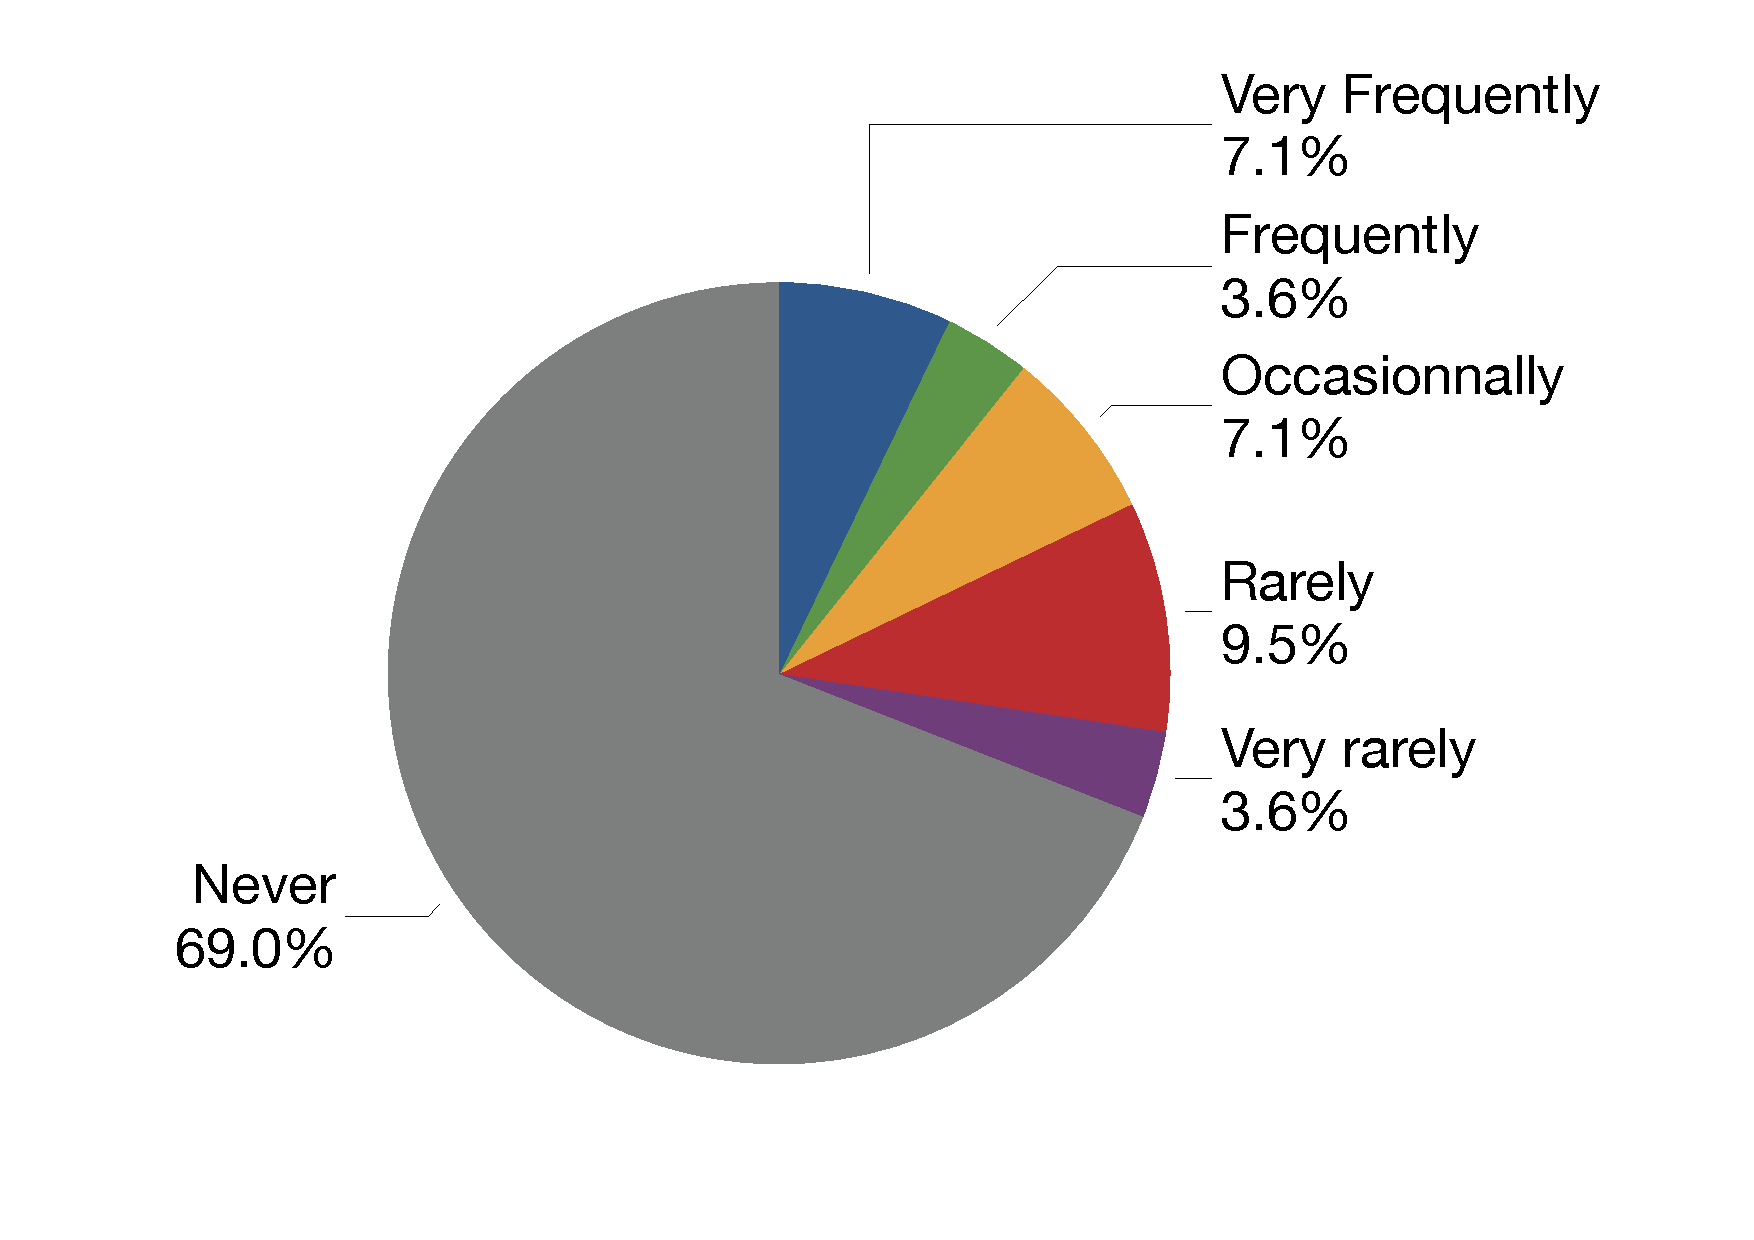
\includegraphics[width=.75\linewidth]{survey_license_check_2}
		\caption{Group 2}
		\label{fig:survey_license_check_2}
	\end{subfigure}
	\caption{Frequency of the answerers checking license of their code snippets against Stack Overflow's CC BY-SA 3.0.}
	\label{fig:survey_license_check}
\end{figure}

We asked the answerers a follow-up question of how frequently they checked for a conflict between software license of the code snippets they copied to their answers and Stack Overflow's CC BY-SA 3.0. As shown in Figure~\ref{fig:survey_license_check}, 67.9\% -- 69\% of answerers from both groups did not perform the checking. There are only approximately 10\% of the answerers who frequently checks for licensing conflicts when they copy code snippets to Stack Overflow.

\vspace{0.5cm}
\noindent\fbox{%
	\parbox[c][1.5cm]{0.98\textwidth}{%
		\textit{For RQ3, approximately 60\% of answerers are aware of CC BY-SA 3.0 license enforced by Stack Overflow. However, 98--99\% of the answerers do not include software license in their Stack Overflow snippets nor check for licensing conflicts when they copy code snippets to Stack Overflow answers.}
	}%
}
\vspace{0.5cm}


In addition, we invited the answerers to give comments regarding their concerns when answering Stack Overflow (SO) with code snippets. Some interesting comments are selected and discussed belwo. The full set of answers can be found in the Appendix~\ref{appendixC}.

\begin{itemize}[label={}]
	\itemsep1em
	\item Comment 1: The answerer addresses a concern of reusing the code snippet without understanding. Moreover, he or she discusses a ramification of low-quality snippets or outdated code containing security issues.
	
	\begin{quote}\textit{The real issue is less about the amount the code snippets on SO than it is about the staggeringly high number of software ``professionals'' that mindlessly use them without understanding what they're copying, and the only slightly less high number of would-be professionals that post snippets with built-in security issues.  A related topic is beginners who post (at times dangerously) misleading tutorials online on topics they actually know very little about. Think PHP/MySQL tutorials written 10+ years after \texttt{mysql\_*} functions were obsolete, or the recent regex tutorial that got posted the other day on HackerNew (\url{https://news.ycombinator.com/item?id=14846506}). They're also full of toxic code snippets.}\end{quote}
	
	\item Comment 2: The answerer suggests that a guidance from Stack Overflow regarding software license will be beneficial.
	
	\begin{quote}\textit{When I copy code it's usually short enough to be considered ``fair use'' but I am not a lawyer or copyright expert so some guidance from SO would be helpful. I'd also like the ability to flag/review questions that violate these guidelines.}\end{quote}
	
	\item Comment 3: The answerer addresses a concern of code understanding.
	
	\begin{quote}\textit{My only concern, albeit minor, is that I know people blindly copy my code without even understanding what the code does.}\end{quote}
	
	\item Comment 4: The answerer discusses a problem from outdated code and his/her solution.
	
	\begin{quote}\textit{The main problem for me/us is outdated code, esp. as old answers have high Google rank so that is what people see first, then try and fail. Thats why we're moving more and more of those examples to knowledge base and docs and rather link to those.}\end{quote}
	
	\item Comment 5: The answerers gives insights into the quality of the Stack Overflow code snippets.
	
	\begin{quote}\textit{Lot of the answers are from hobbyist so the quality is poor. Usually they are hacks or workarounds (even MY best answer on SO is a workaround).}\end{quote}
\end{itemize}

%\subsection{Visitor Responses}
%
%To answer RQ4 and RQ5, we ask Stack Overflow visitors about their experiences of outdated code and their awareness to software license of Stack Overflow code snippets. We received 89 answers from 5 groups of Stack Overflow visitors. The combined results and discussions are presented below.
%
%\subsubsection*{RQ4: Are Stack Overflow visitors aware of outdated code on Stack Overflow?}
%
%We asked the visitors whether they have any problem from reusing Stack Overflow code snippets and how often did the problems occur. 
%
%\begin{figure}
%	\centering
%	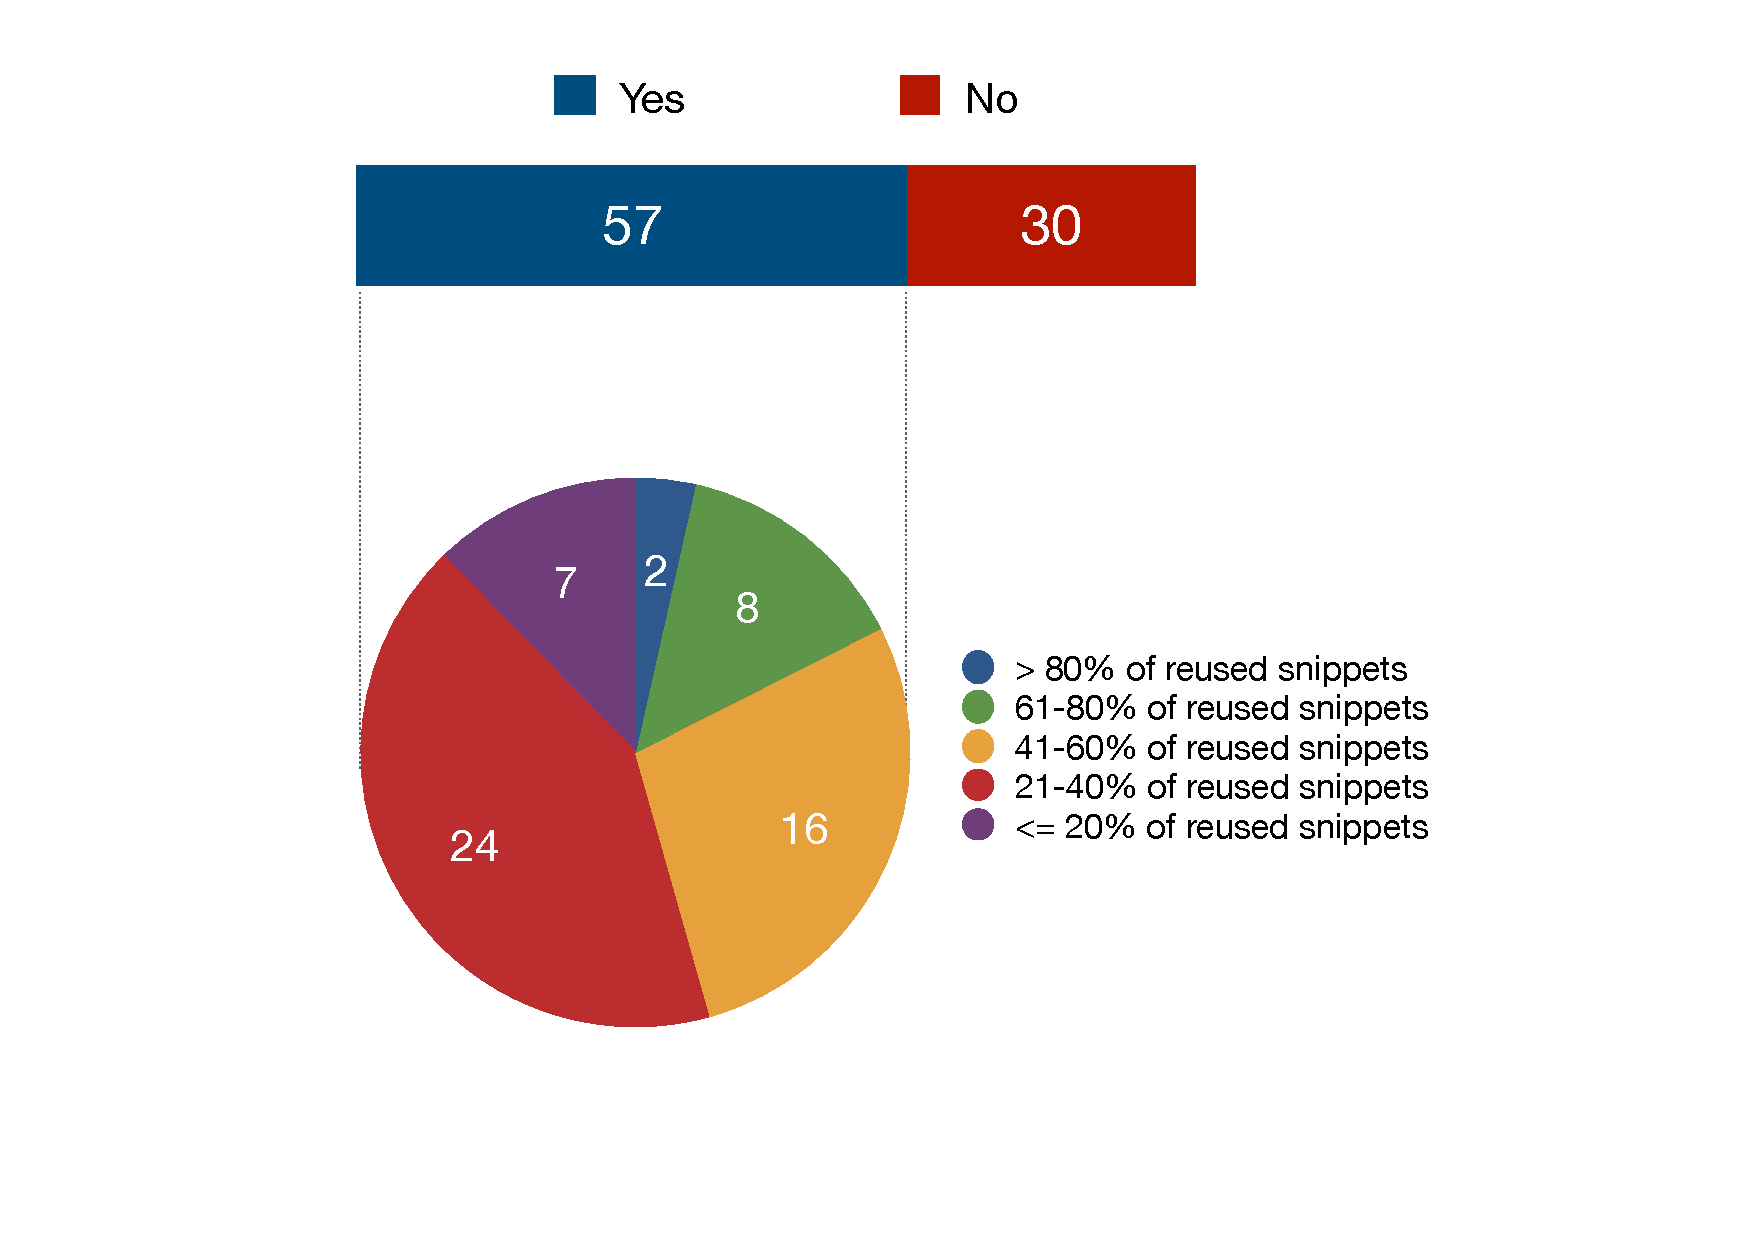
\includegraphics[width=.5\linewidth]{survey_v_problems}
%	\caption{Number of visitors who experienced a problem from reusing Stack Overflow code snippets.}
%	\label{fig:survey_v_problems}
%\end{figure}
%
%
%\vspace{0.5cm}
%\noindent\fbox{%
%	\parbox[c][0.5cm]{0.98\textwidth}{%
%		\textit{For RQ4, }
%	}%
%}
%\vspace{0.5cm}
%
%\subsubsection*{RQ5: Are Stack Overflow visitors aware of software licensing of code snippets from Stack Overflow?}
%
%\vspace{0.5cm}
%\noindent\fbox{%
%	\parbox[c][0.5cm]{0.98\textwidth}{%
%		\textit{For RQ5, }
%	}%
%}
%\vspace{0.5cm}

\section{Related Work}

\subsection{Stack Overflow}

Stack Overflow is a gold mine for software engineering research and has been put
to use in several previous studies. In terms of developer-assisting tools,
Seahawk is an Eclipse plug-in that searches and recommends relevant code
snippets from Stack Overflow~\citep{Ponzanelli2013}. A follow up work, Prompter,
by Ponzanelli et al.~\citep{Ponzanelli2014} achieves the same goal but with
improved algorithms. The code snippets on Stack Overflow are mostly examples or
solutions to programming problems. Hence, several code search systems use whole
or partial data from Stack Overflow as their code search
databases~\citep{Keivanloo2014,Park2014,
	Stolee2014,Subramanian2013,Diamantopoulos2015}. Furthermore, Treude et
al.~\cite{Treude2016}~use machine learning techniques to extract insight
sentences from Stack Overflow and use them to improve API documentation.

Another research area is knowledge extraction from Stack Overflow.
\cite{Nasehi2012}~studied what makes a good code example by analysing answers
from Stack Overflow. Similarly, \cite{Yang2016} report the number of reusable
code snippets on Stack Overflow across various programming languages.
\cite{Wang2013_StackOverflow} use Latent Dirichlet Allocation (LDA) topic
modelling to analyse questions and answers from Stack Overflow so that they can
automatically categorise new questions. There are also studies trying to
understand developers' behaviours on Stack Overflow, e.g.~A study by
\cite{Movshovitz-Attias2013,Rosen2016,Choetkiertikul2015,Bosu2013}.
\cite{Yang2017} analysed 909k non-fork Python projects on Github and 1.9
million python code snippets on Stack Overflow and found thousands of 
code blocks that are copied from Stack Overflow to GitHub.

\subsection{Software Licensing}
Software licensing is crucial for open source and industrial software
development. Di Penta et al.~\cite{DiPenta2010} studied the evolution of
software licensing in open source software and found that licensing statements
change over time. \cite{German2009} found that licensing conflicts occur between
the clone siblings, i.e.~clones among different systems that come from the same
source. Later, \cite{German2010} created an automated tool for software license
identification, Ninka. \cite{An2017} detected clones between 399 Android apps
and Stack Overflow Java code snippets. They found that  that 1,279 cloned
snippets potentially violate software licenses. Our study gives insights into
the software licensing of Stack Overflow code snippets. We study the licensing
awareness of developers when they copy and paste code to/from Stack Overflow.

\subsection{Reusing of outdated third-party source code} 
Outdated code occurs in software development. Xia et al.~\cite{Xia2014} discover
that there are code reused from popular open source projects in a large number
of open source systems. More importantly, some of the reused code are outdated
which affect quality and security of the software. Our study focuses on a
similar problem but on the context of Stack Overflow.

\section{Conclusions}

We present our online survey results of Stack Overflow answerers in terms of their awareness to outdated code snippets and their software license.


%\bibliographystyle{abbrv}
%\bibliographystyle{plainnat}
\bibliographystyle{spbasic}
\bibliography{sigproc} 

\clearpage
\section{Appendix}

This appendix contains additional materials of the Stack Overflow answerer survey questions, the visitor survey questions, and the complete set of open comments from the Stack Overflow answerers.

\clearpage

\appendix
\section{Stack Overflow Answerer Survey}\label{appendixA}
\begin{figure}[H]
	\centering
	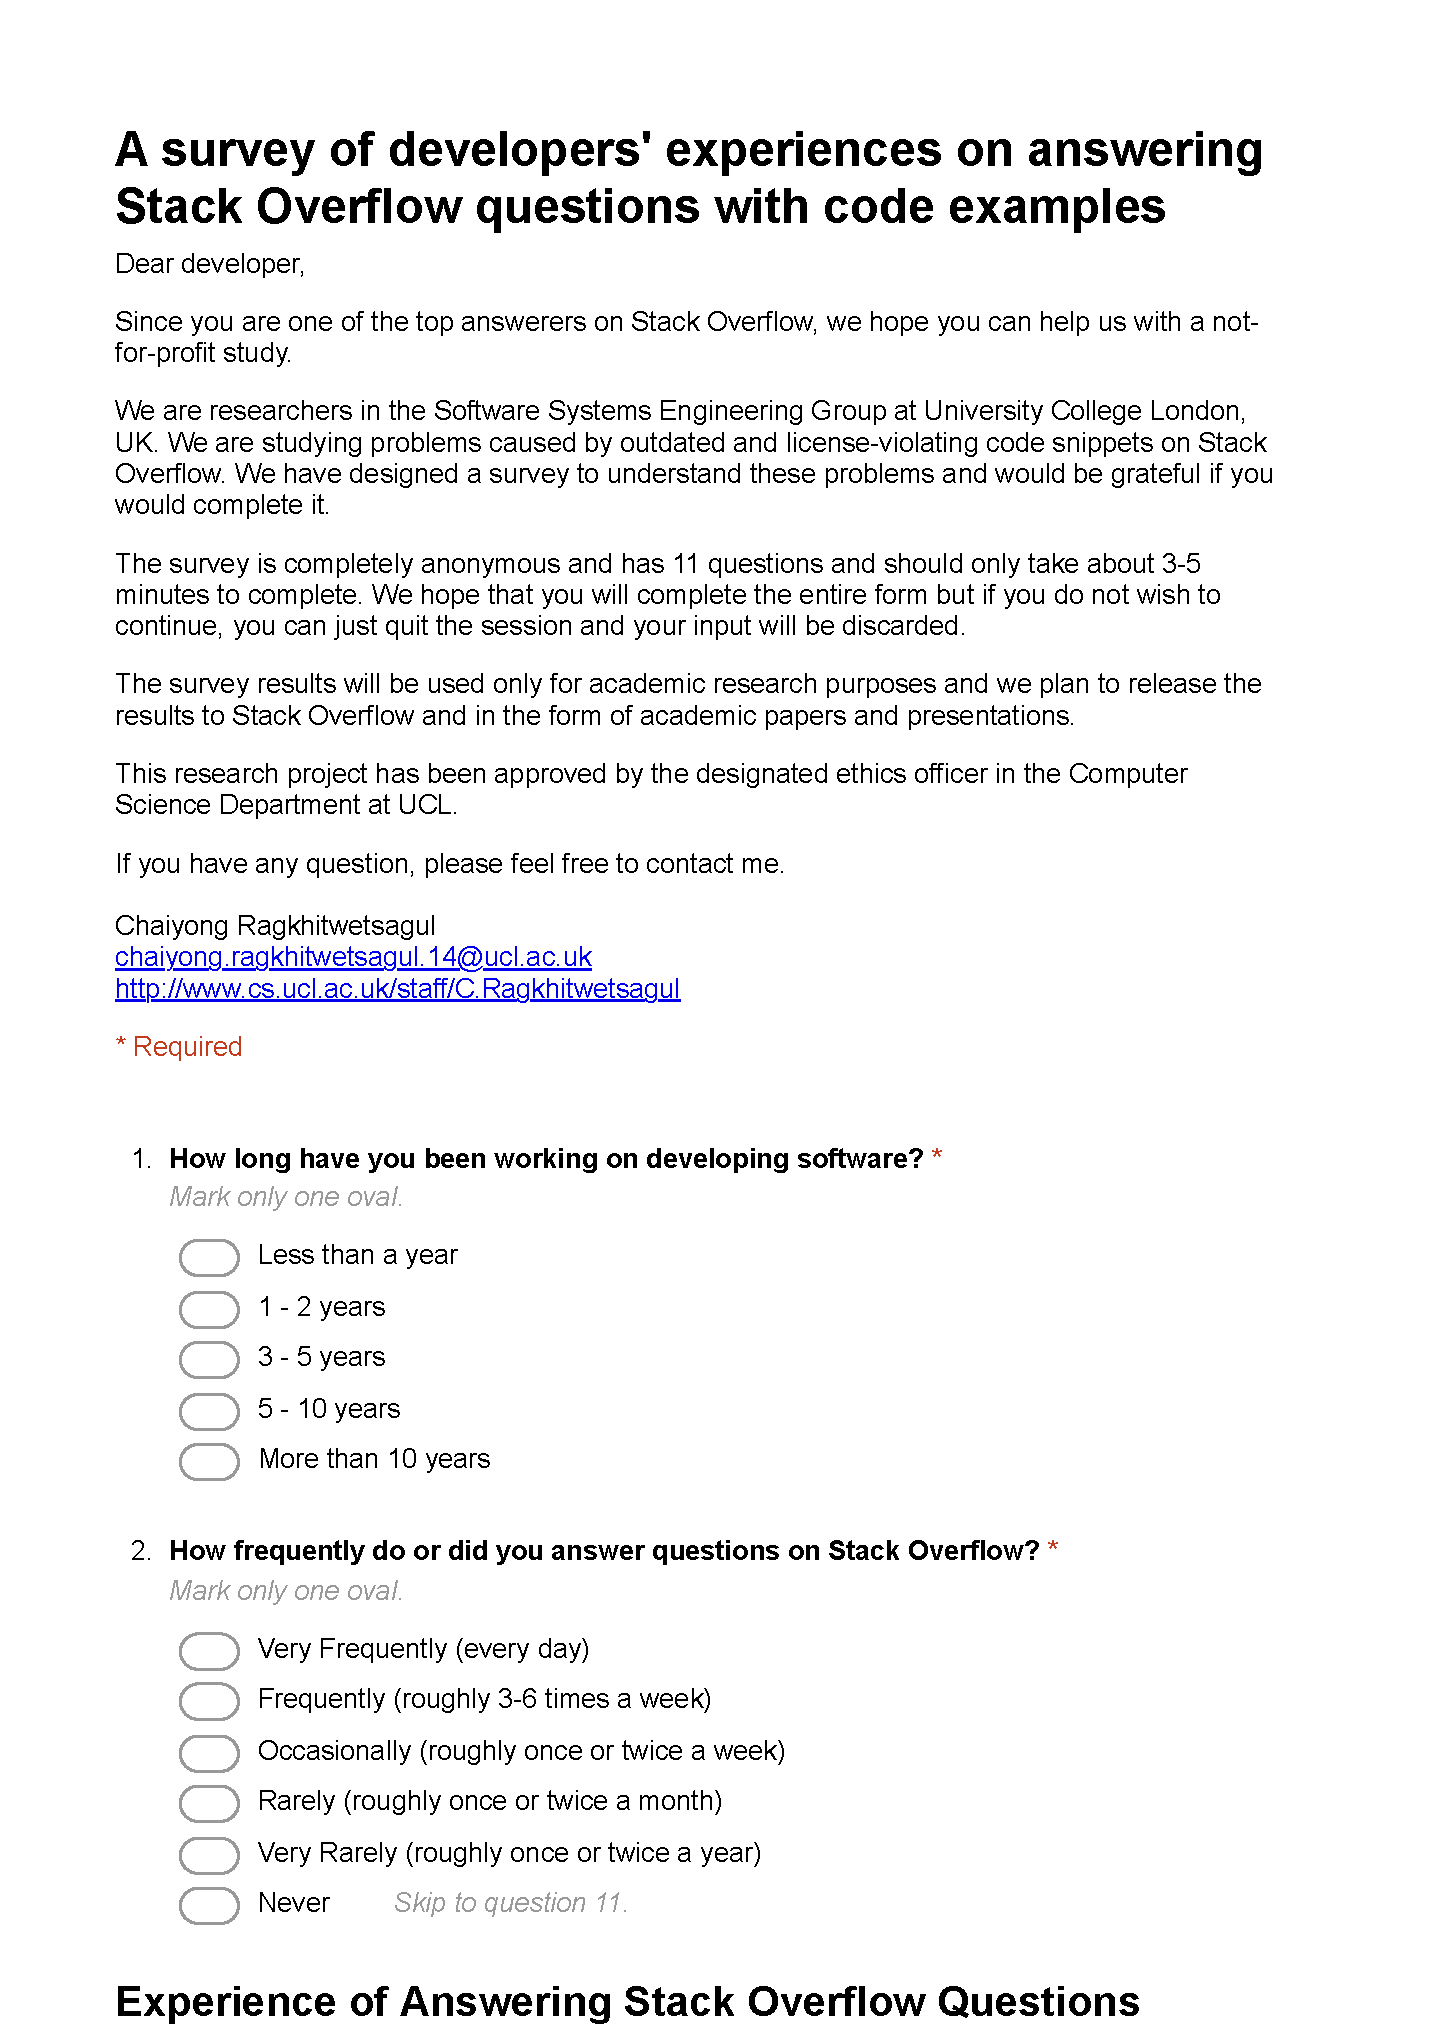
\includegraphics[width=0.8\linewidth]{answerer-1}
	\label{fig:answerer-1}
\end{figure}

\begin{figure}[H]
	\centering
	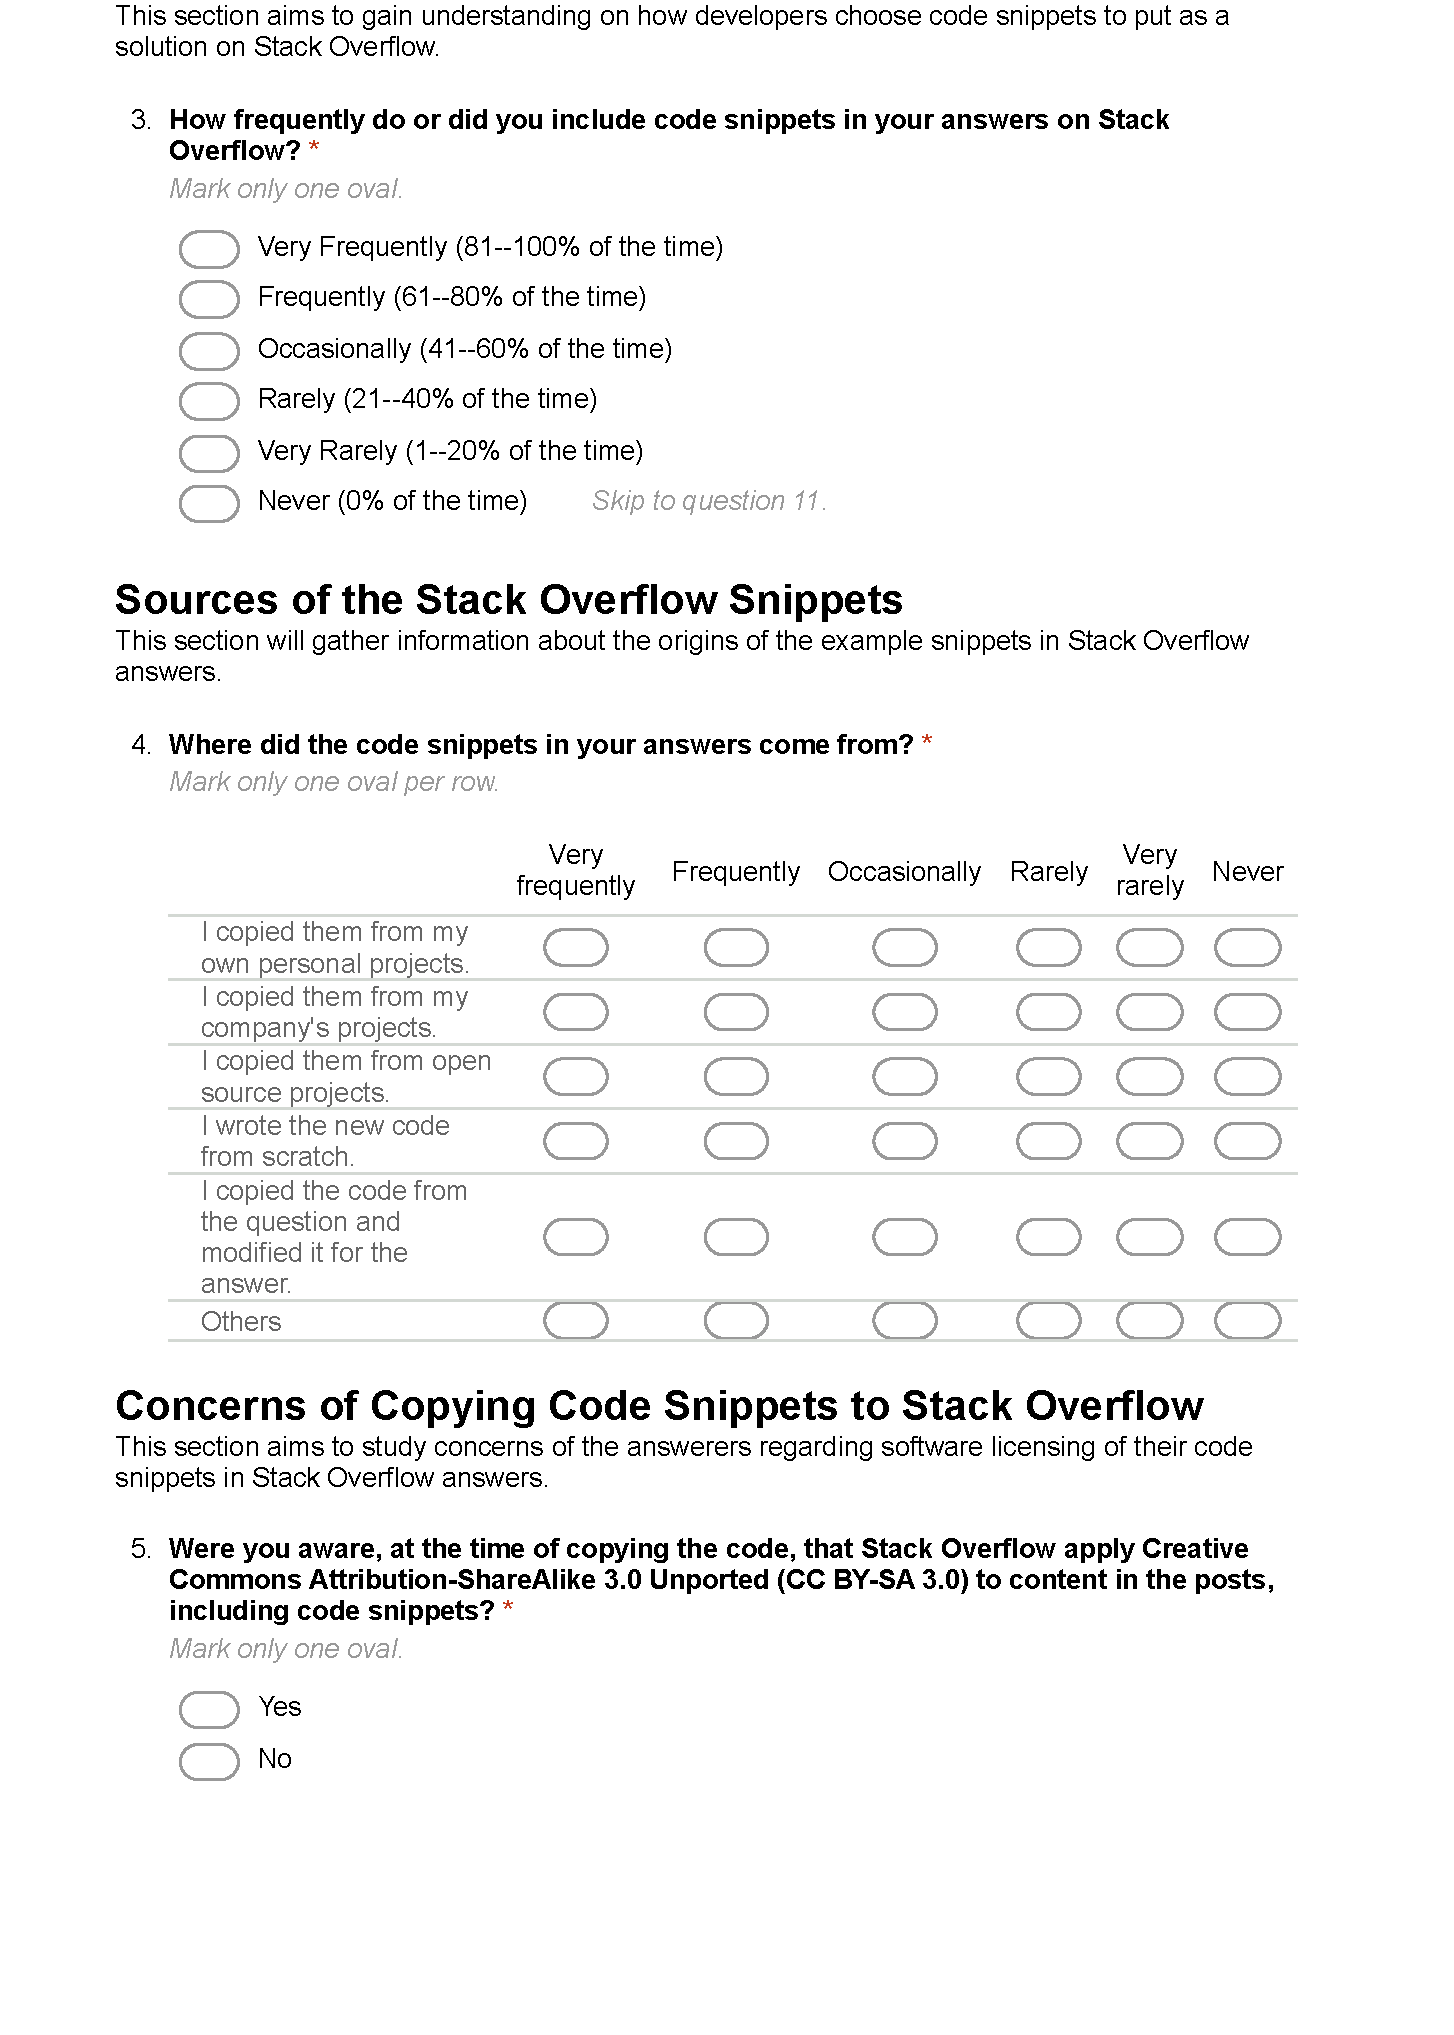
\includegraphics[width=0.9\linewidth]{answerer-2}
	\label{fig:answerer-2}
\end{figure}

\begin{figure}[H]
	\centering
	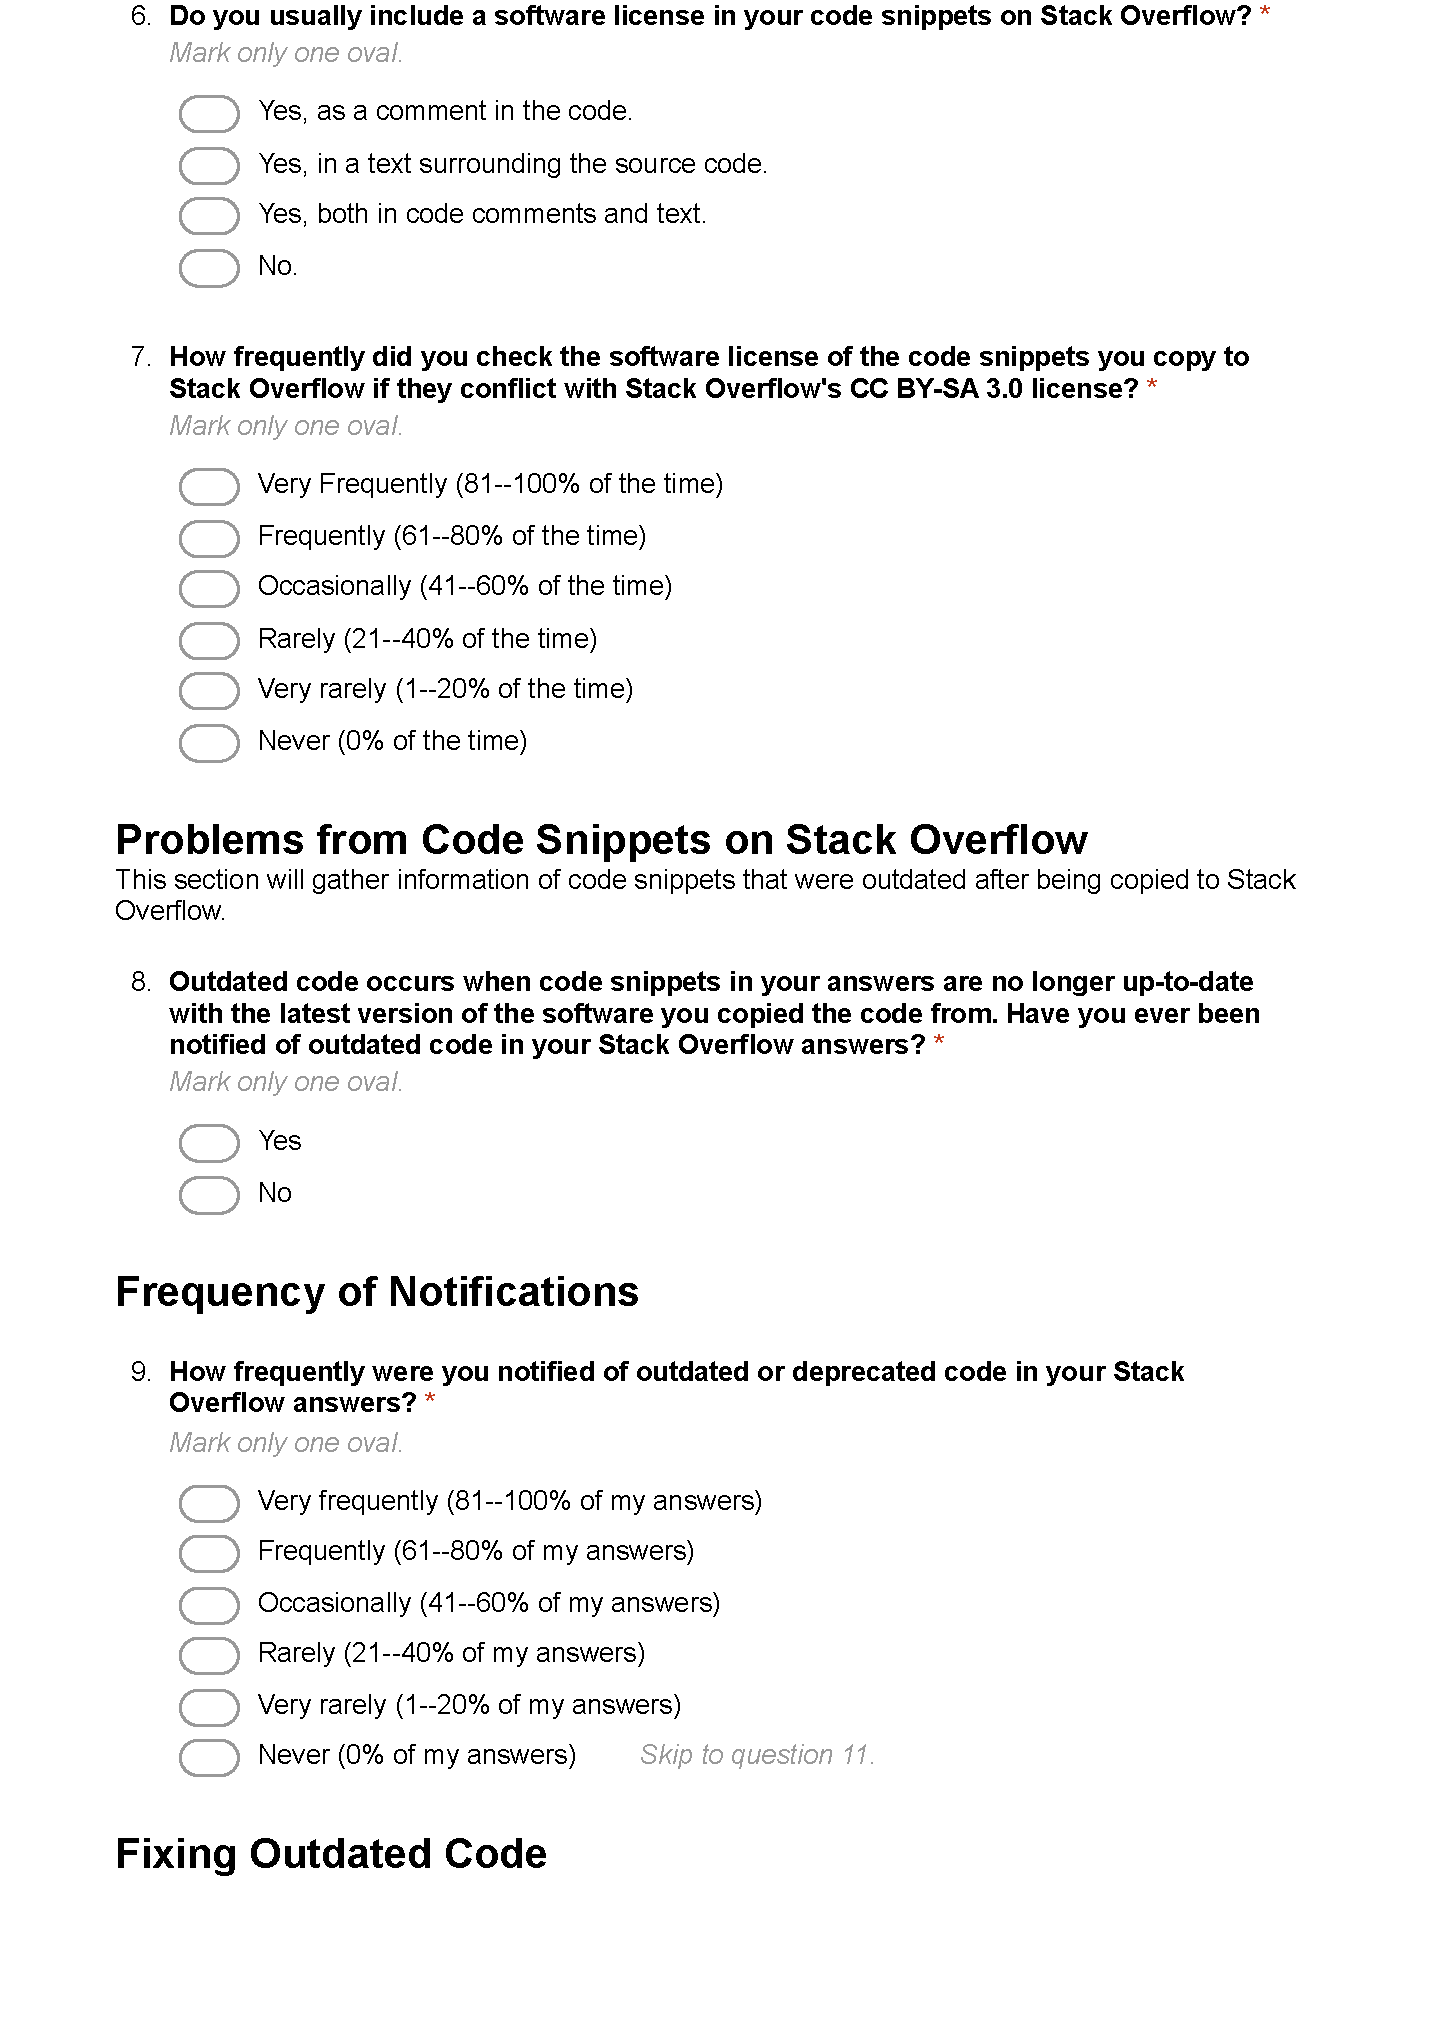
\includegraphics[width=0.9\linewidth]{answerer-3}
	\label{fig:answerer-3}
\end{figure}

\begin{figure}[H]
	\centering
	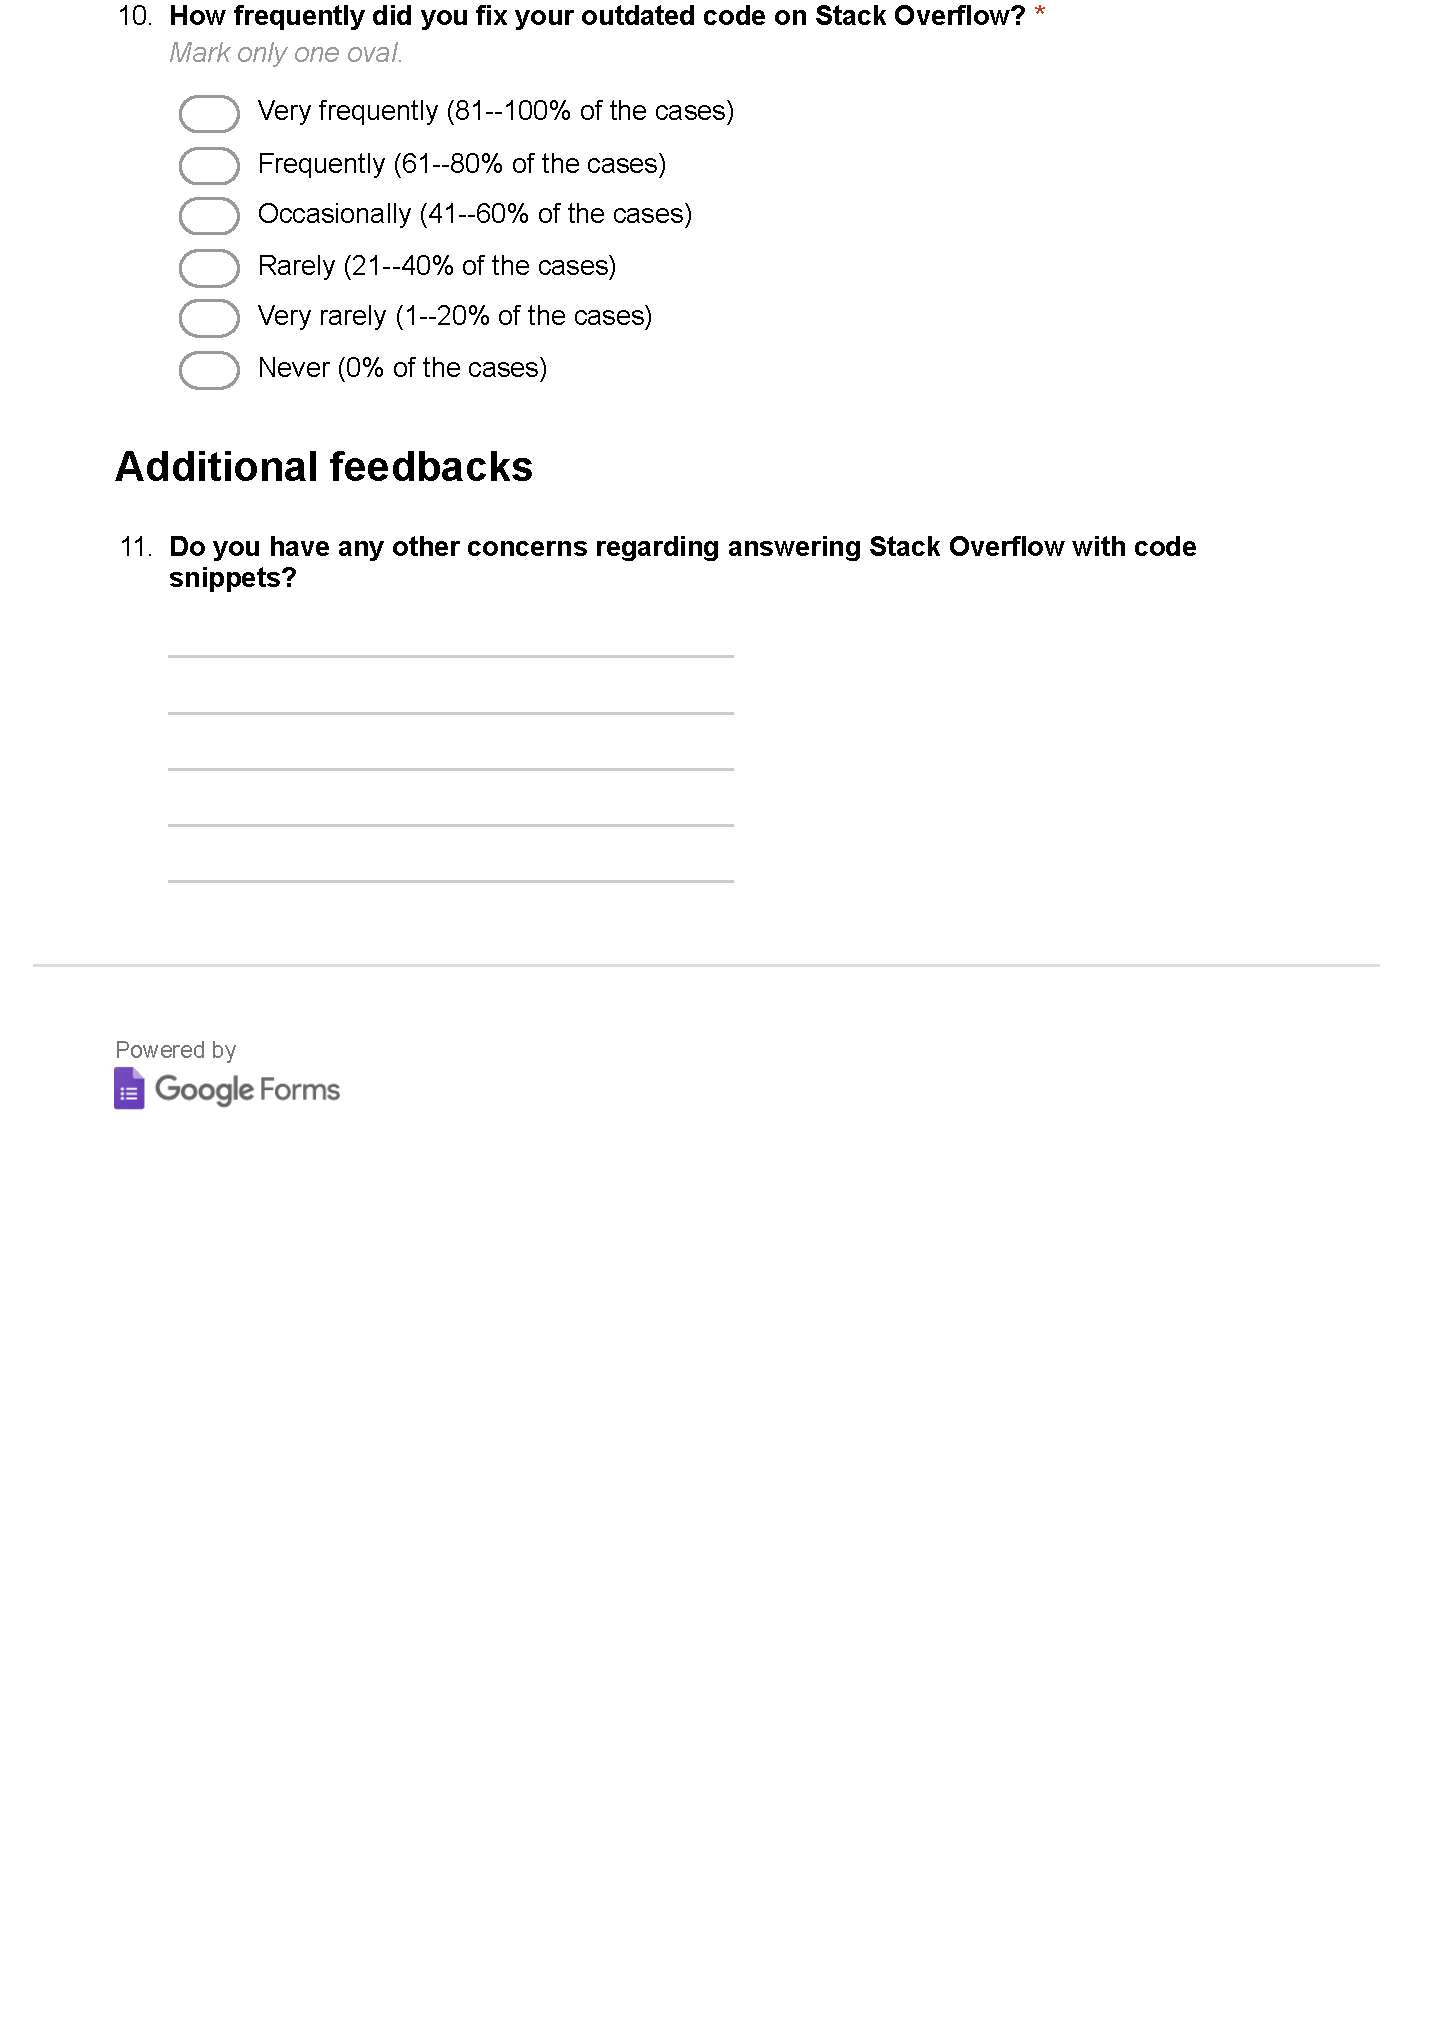
\includegraphics[width=0.9\linewidth]{answerer-4}
	\label{fig:answerer-4}
\end{figure}

%\section{Stack Overflow Visitor Survey}\label{appendixB}
%\begin{figure}[H]
%	\centering
%	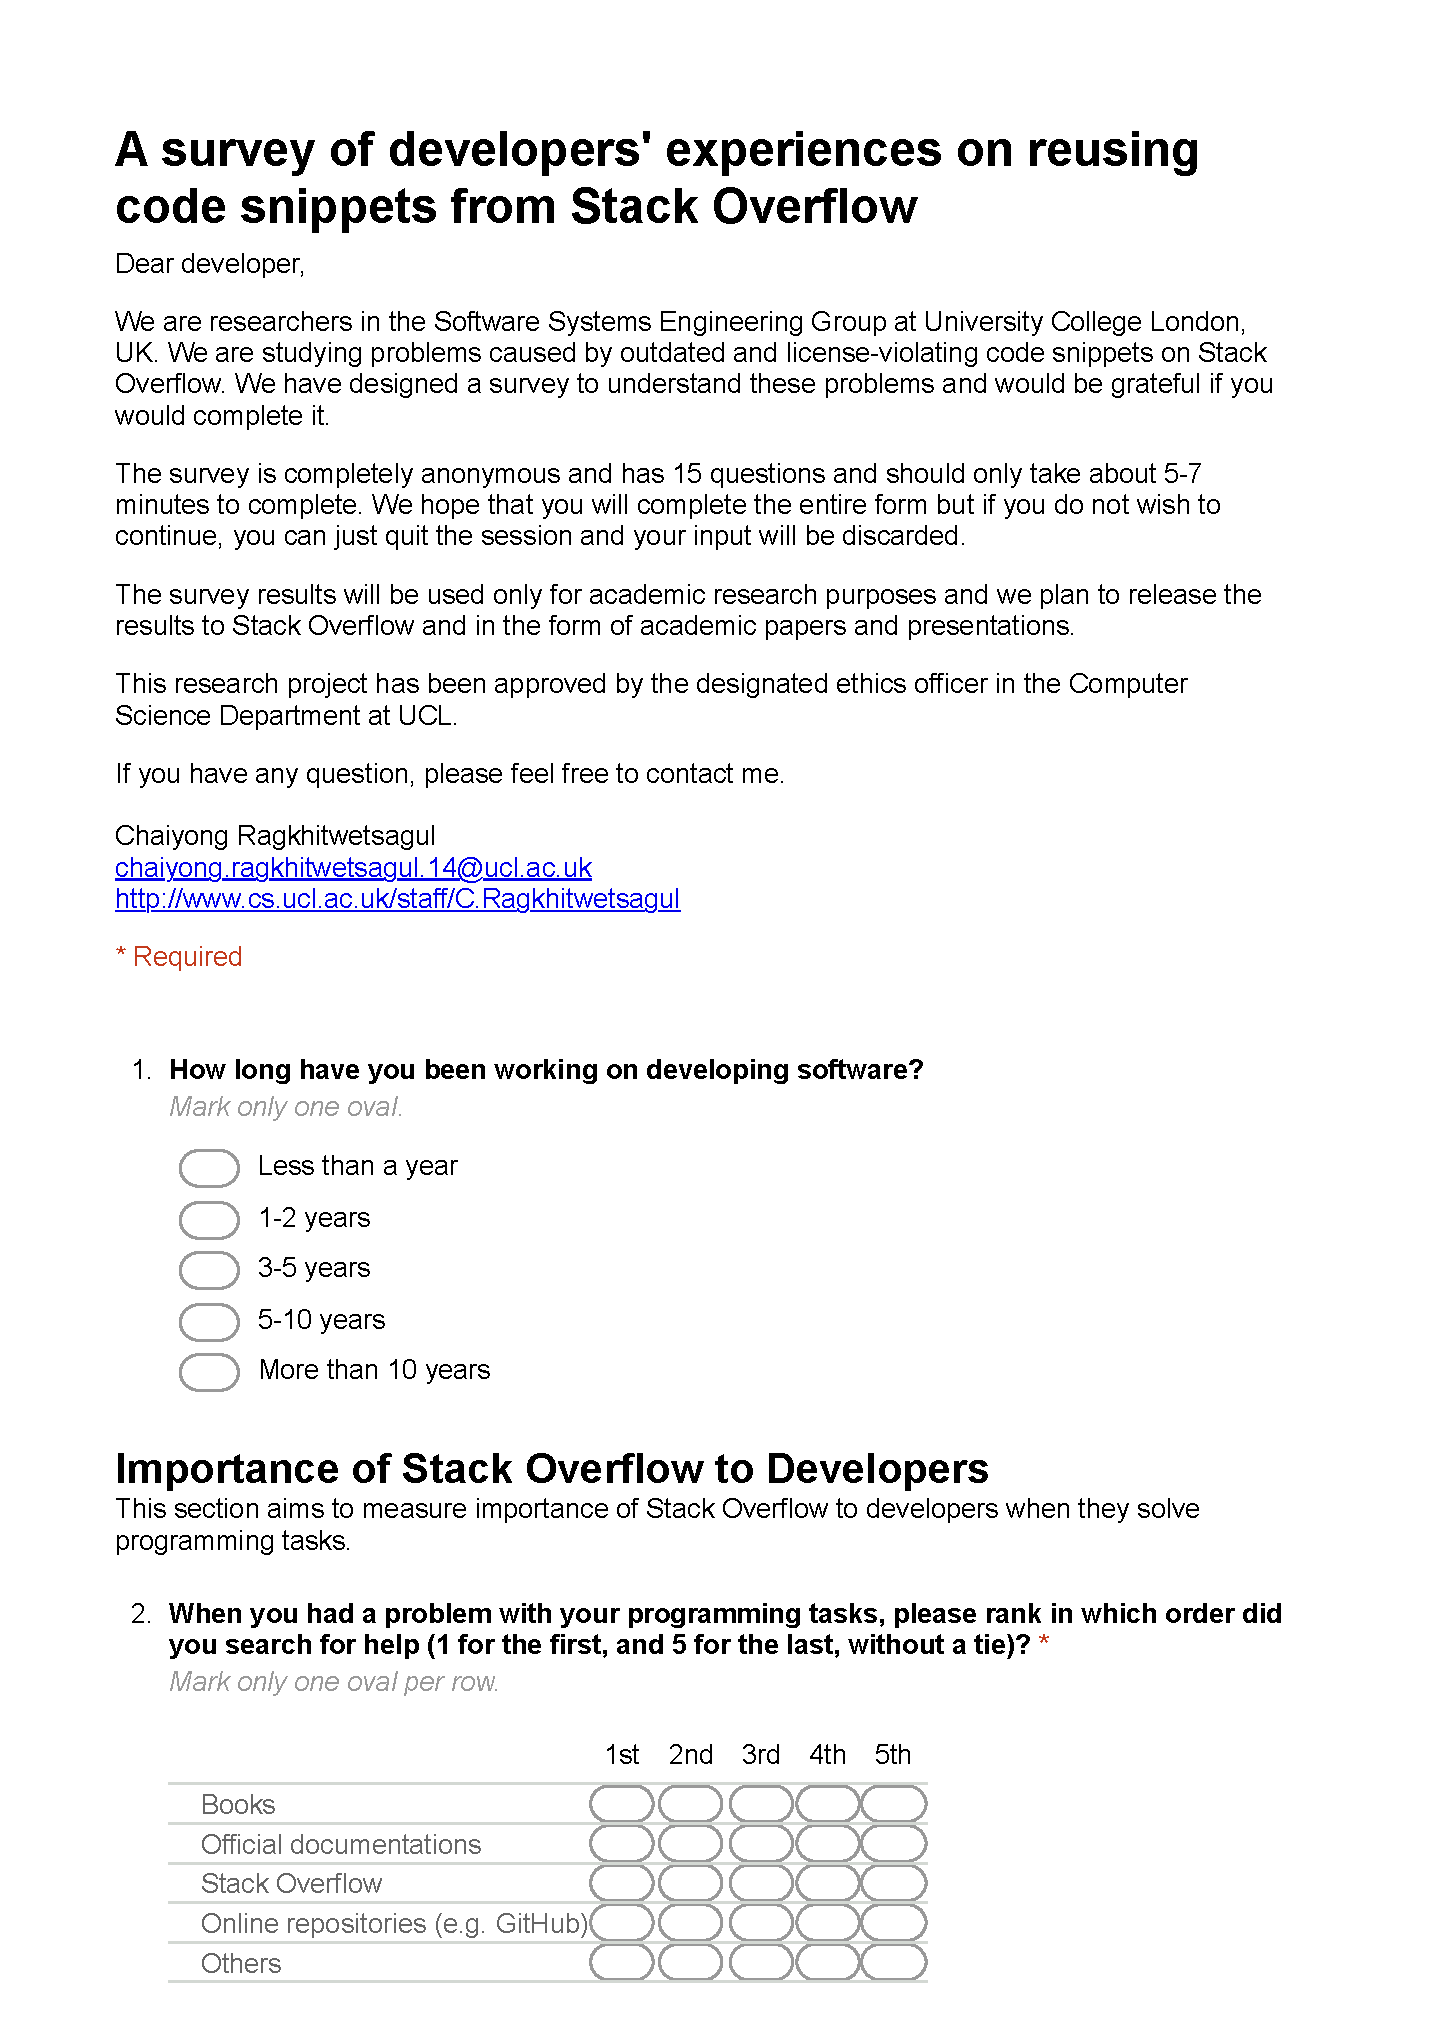
\includegraphics[width=0.85\linewidth]{visitor-1}
%	\label{fig:visitor-1}
%\end{figure}
%
%\begin{figure}[H]
%	\centering
%	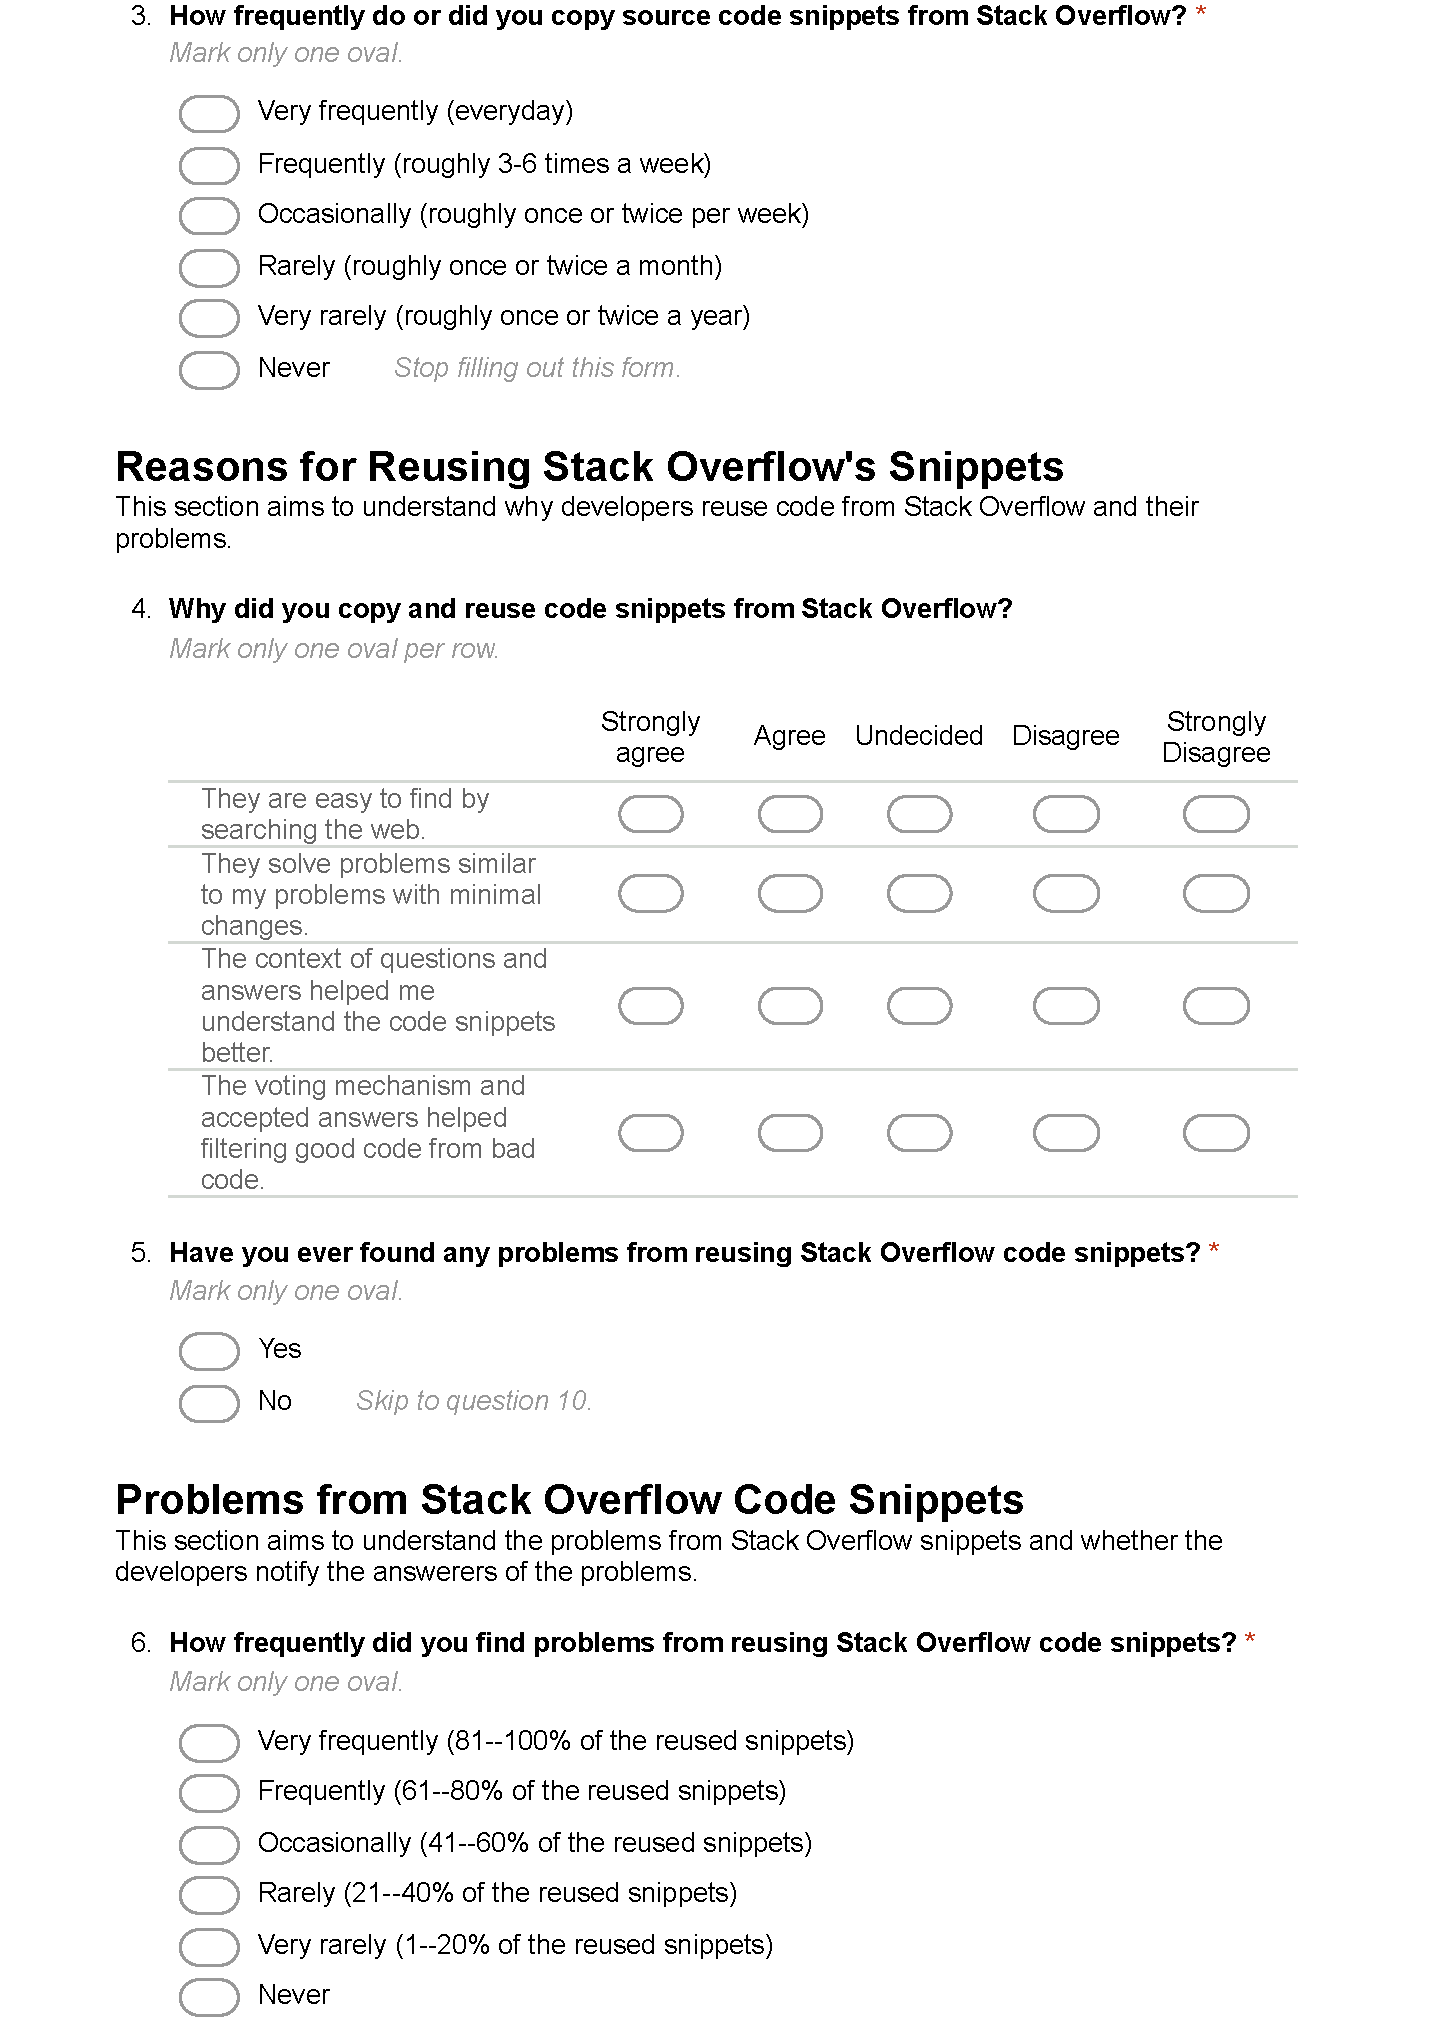
\includegraphics[width=0.9\linewidth]{visitor-2}
%	\label{fig:visitor-2}
%\end{figure}
%
%\begin{figure}[H]
%	\centering
%	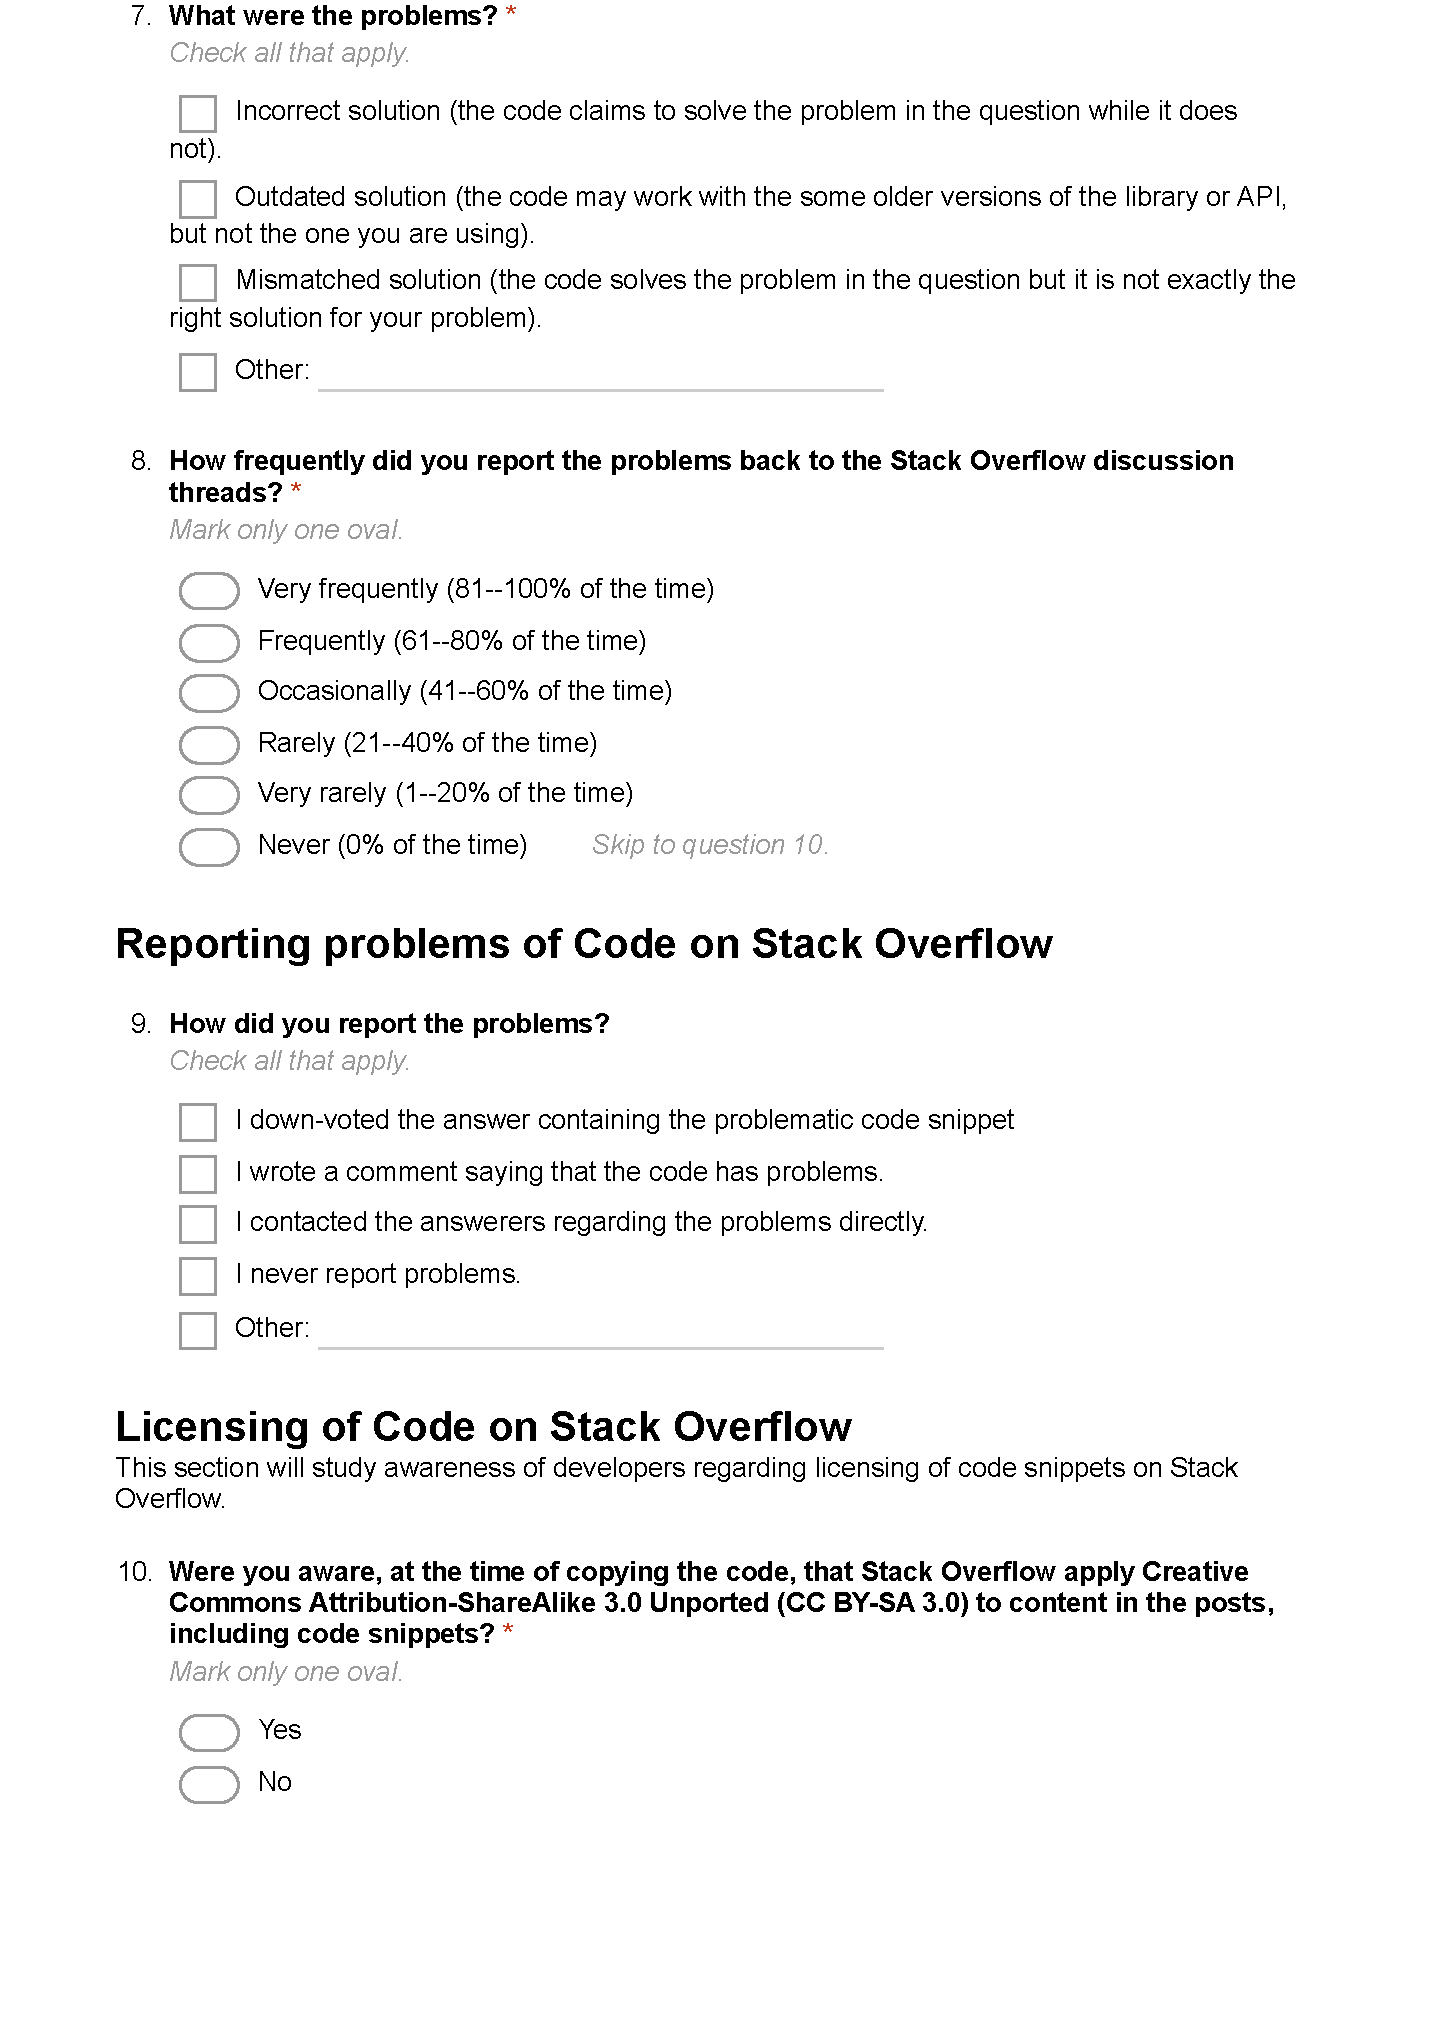
\includegraphics[width=0.9\linewidth]{visitor-3}
%	\label{fig:visitor-3}
%\end{figure}
%
%\begin{figure}[H]
%	\centering
%	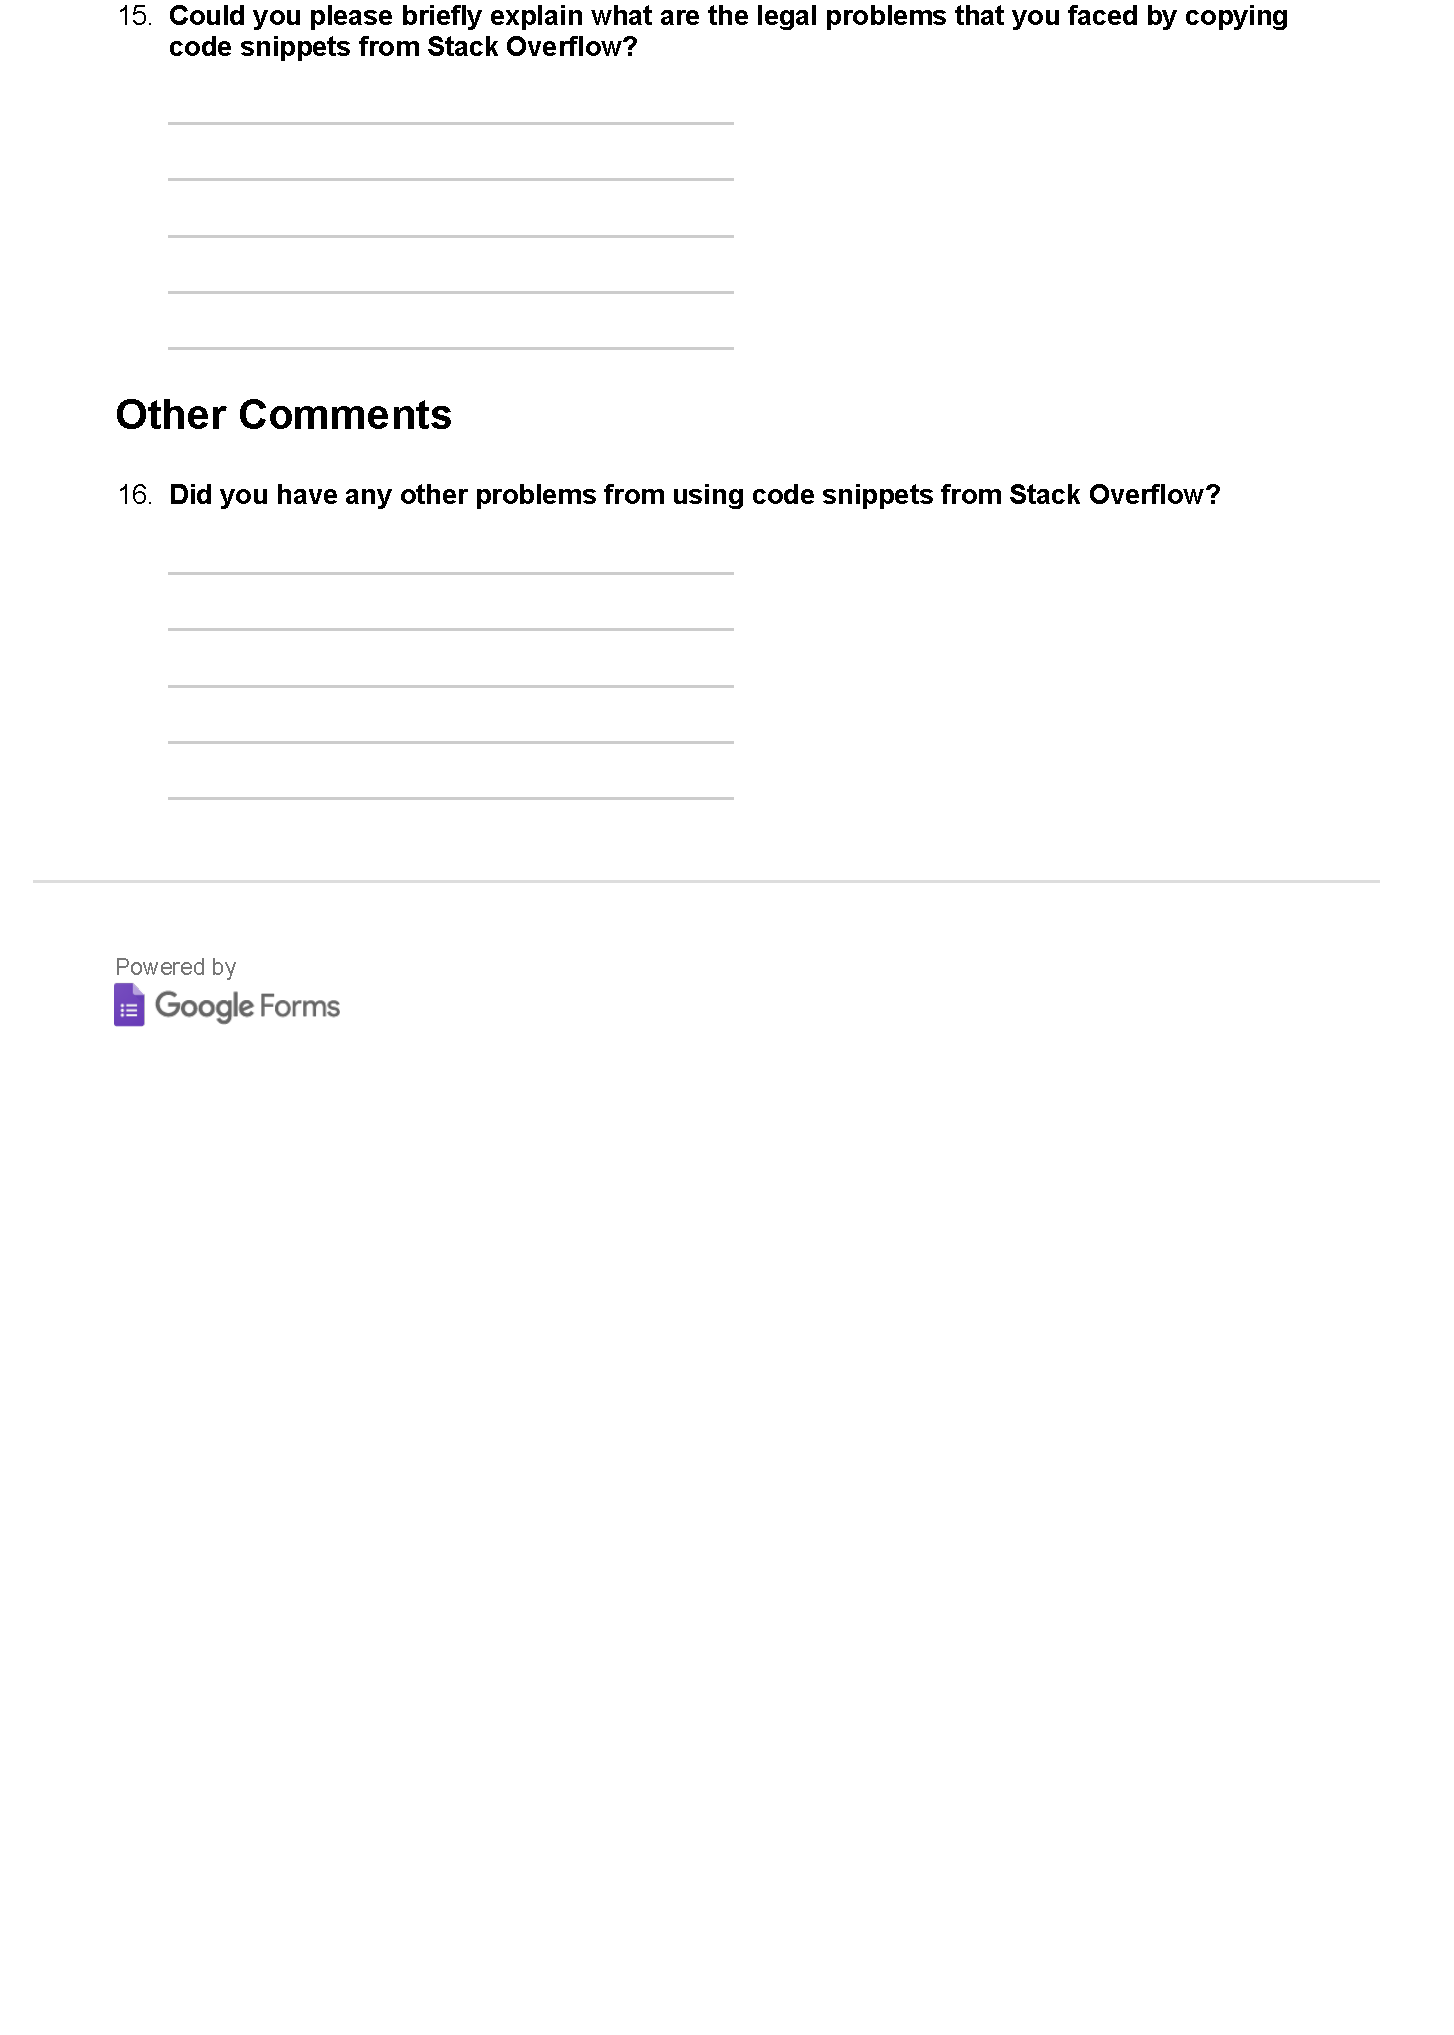
\includegraphics[width=0.9\linewidth]{visitor-4}
%	\label{fig:visitor-4}
%\end{figure}

\section{Open Comments from Stack Overflow Answerers}\label{appendixC}

\begin{enumerate}
	\itemsep1em
	\item Sometimes you have to post code from official documentation, like in case of C\#, code form MSDN is posted in the answer with added explanation.
	\item Snippets on SO are usually for demonstrating a technique and therefore age well. If otherwise, I usually made them a gist, codebin or jsfiddle.
	\item The real issue is less about the amount the code snippets on SO than it is about the staggeringly high number of software ``professionals'' that mindlessly use them without understanding what they're copying, and the only slightly less high number of would-be professionals that post snippets with built-in security issues.
	\item A related topic is beginners who post (at times dangerously) misleading tutorials online on topics they actually know very little about. Think PHP/MySQL tutorials written 10+ years after \texttt{mysql\_*} functions were obsolete, or the recent regex tutorial that got posted the other day on HackerNew (\url{https://news.ycombinator.com/item?id=14846506}). They're also full of toxic code snippets.
	\item Just to say: the reason that I very rarely check the license status is that the code I am posting is almost always my own or adapted from the question, or imported from an open source project that I have worked on and already know the license terms, or from my own company code that I can 100\% say it is OK to post in public because I know our policies.
	\item No. Code snippets are short and small enough that no IP can be in them.
	\item The point of snippets are that they are trivial. I mostly write from scratch or copy-\&-fix a snippet from the question. Most are illustrative or incomplete --- they aren't of any value at all in isolation. They rarely take more than a few minutes to write, and it's usually harder to explain what they're doing in plain English. Where something is large enough to worth the effort of licensing then it's far too big for a snippet. In those cases I create a GitHub project (with a license) and link to it. I'd be wary of increased IP controls --- I doubt there is value they could add to snippets, but they could create significant barriers to contributors, which would hurt the site.
	\item I always try to see what kind of person is asking the question. If it is a student, I don't want to just hand out the answer; they will learn nothing from that. If, on the other hand, it's somebody looking for best practices or a clever trick, I'm not too worried about giving out the solution. In this case, chances are much higher that the person asking the question will go ``Ahh, yes, of course!'' and understand the question, whereas some students are more likely to mindlessly copy-paste the answer.
	\item However, it is also a competitive site, so if your answer requires too much work to incorporate, it won't get accepted or upvoted. As a result, some people---I'm guilty of this myself, I'm sure---will hand out an answer willy-nilly that might solve the problem at hand, but in the long run be a disservice to the person asking.
	\item But I digress: My point is that it's sometimes better to describe a solution rather than just hand off a code snippet. However, since your project seems to pertain to copyright issues, I suppose that's not relevant to you.
	\item I'm not sure it's possible to include a license in your questions/answers. I'm not sure what the legal ramifications would be if you tried it, since you already agreed to S.O.'s terms. This is a very interesting question and I look forward to hearing the results of your research.
	\item I think it's important to realise the code snippets are designed to be very small, useful to illustrate concepts (10 lines or less). When you consider licensing laws of such a small amount of code, while technically may be violating a licence, in practice it would be nearly impossible to enforce such a claim.
	\item SO code snippets are great but there is lot to improve . It's hard to edit and see output in so but website like jsfiddle , jsbin provide nice interface where code editing and output is easy to do.
	\item Outer thing is in so lot of code snippets doesn't work because some users don't add libraries like angular, jquery. I think it's better if we can identify and ask user to auto inject relevant libraries.
	\item Code snippets are usually just a few lines of code so it will be hard to enforce any copyright claims except when it is a method used for something company-specific (such as generating encryption keys). Regardless, since most of the code I write is specifically to answer a given question and having full knowledge of the license system used by Stack Overflow, it is entirely unimportant to concern myself with licensing the code provided. Also, code from MSDN documentation which I sometimes adapt and modify for answers are already in the public domain so it makes no sense re-licensing it.
	\item On the matter of deprecation, I almost entirely use .NET which has got different versions of the framework. Therefore, code deprecation is not often a problem since what is deprecated on one version of the framework may be the only way of solving a given problem on an older version of the framework. I may also have to add that questions I tend to answer are about how to solve general coding problems so they are not usually subject to deprecation.
	\item I think you're forgetting the fact that as a community, we want to share knowledge. Patents, copyright issues and so on --- it's all just annoying. We're there to have fun and to share knowledge with people. 
	\item In the early days, the internet used to be full of free-for-all stuff without any licenses. Because of that, it was a fantastic tool to share knowledge and information on a vast scale. The remnant of this, open source, couldn't have existed without this!
	\item Personally, I believe this ``intellectual property'' drive of the last decade is completely overrated. If you make something \textbf{substantial}, it's fine to be able to claim some ownership --- but on snippets? It's like patenting the stuff you make in your free time in your shed... it doesn't make sense and just adds to the pile of legal bullshit imho.
	\item No. I only put code on there that I have the right to (code I created or have permission to share). Adding the code is not an issue for me.
	\item When I copy code it's usually short enough to be considered ``fair use'' but I am not a lawyer or copyright expert so some guidance from SO would be helpful. I'd also like the ability to flag/review questions that violate these guidelines.
	\item The snippets are all small enough that I reckon they fall under fair use.
	\item I always try and attribute the code I take from other places. I feel pointing back to the origin should be sufficient in terms of giving credit where it's due. Open source is about the sharing of ideas so that others can build on them. Education is a primary use case of open source in my opinion.
	\item My only concern, albeit minor, is that I know people blindly copy my code without even understanding what the code does.
	\item This survey may be inapplicable to me because I never copy code from existing projects.
	\item Stack Overflow did an effort to apply a MIT license to all code snippets, while keeping CC-SA for the text content. Too bad they didn't succeed with it, as it would have solved many issues.
	\item The main problem for me/us is outdated code, esp. as old answers have high Google rank so that is what people see first, then try and fail. Thats why we're moving more and more of those examples to knowledge base and docs and rather link to those.
	\item I've got no issues with code snippets on Stack Overflow, I think they are great. Any one using them should pay attention to details such as the date of the answer etc.
	\item SO's license is not clearly explained when one registers or starts to answer questions.
	\item No, most copied code snippets are so trivial that licensing them would be nearly impossible. It's also mostly modified version, where only some patterns are used.
	\item Lot of the answers are from hobbyist so the quality is poor. Usually they are hacks or workarounds (even MY best answer on SO is a workaround).
	\item I think most example and explanatory snippets don't need a code-specific license. The CC license provides just fine. The examples either aren't copyrightable in the first place, or merely used as starting point (not used exactly as-is, not very different from reading an ``All rights reserved'' education book when learning programming, and ``using'' it in your career every day going forward). In addition, there is also the attitude of authors. Where I might care about attribution for distribution of my answer, the code within my answer is always Public Domain for me, meaning, I would never defend it. (I used to state that on my profile as well, but not in every post.)
	\item Correctness and even syntax are often in doubt if I haven't had time to test the snippet end-to-end under the OP's conditions/environment.
	\item It will be awesome if it becomes simple git repositories like github's gist.
	\item Note that although I was not specifically of SO's licensing terms, I did have an in mind what those terms were likely to be. I have always made sure that there should be no reason that I should not share the code that I included in my replies.
	\item It's an ESSENTIAL part of the site, it would NEVER work without such pieces of code. Also, given the snippets are very small in 99.99\% of cases, legal aspects of this are inherently and pretty much always overlooked by the users.
\end{enumerate}

\end{document}
% end of file template.tex

